\documentclass[12pt]{article}
\usepackage[margin=15mm]{geometry}
\usepackage{graphicx}
\usepackage{url}
\graphicspath{{../../}} %%%goes to the path: docs/

\title{
Supplementary Material
}
\author{Miguel Xochicale}
\date{ \today }

\begin{document}
\maketitle

\begin{abstract}
Report for supplementary material where section 1 describes datasets and section 2 shows surface plots of 3D RQA ENTR values for 3 participants (p01, p02 and p03).
\end{abstract}

\tableofcontents
%\newpage


%%%%%%%%%%%%%%%%%%%%%%%%%%%%%%%%%%%%%%%%%%%%%%%%%%%%%%%%%%%%%%
\section{Datasets}
Datasets are for 
(a) window size of 100, 250, 500 and 750 samples (w100, w250, w500, w750);
(b) smoothness: sg0, sg1 and sg2;
(c) movement: Horizontal Normal (HN), Horizontal Faster (HF), Vertical Normal (VN) and Vertical Faster (VF); and 
(d) sensors: Sensor attached to Human (HS01), sensor attached to Robot (RS01).

The location of the dataset is shown below with the first two lines of xdatav00.dt denoting labels.
\begin{verbatim}
~/srep2021/data/dataset$ tree --si
[ 46M]  xdata_v00.dt
.
.
.
"Participant" "Activity" "Sensor" "Sample" "Time" 
"sg0zmuvGyroY" "sg1zmuvGyroY" "sg2zmuvGyroY" 
"sg0zmuvGyroZ" "sg1zmuvGyroZ" "sg2zmuvGyroZ"
...
"p01" "HN" "HS01" 1 0 
0.0110396263359954 0.00606430191548277 0.0385586376765087 
0.00467559072085554 0.00509907428630649 0.168927517477539
...
\end{verbatim}

%├── [4.1k]  dataset
%│   └── [ 46M]  xdata_v00.dt
%.
%.
%.

%%%%%%%%%%%%%%%%%%%%%%%%%%%%%%%%%%%%%%%%%%%%%%%%%%%%%%%%%%%%%%
\section{3D RQA ENTR values}
Location of code, data and figures for 3D RQA ENTR values is shown below 
\begin{verbatim}
## Code
$HOME/srep2021/code/rscripts/G_3Drqa
`> source(  paste( getwd(), '/C_3Drqa_plots_epsilons.R', sep=''), echo=TRUE )`

## Data
$HOME/srep2021/data/rqa$ tree -s 

## Figures
$HOME/srep2021/docs/figures/rqa/src/3drqa_epsilons$ tree -s
\end{verbatim}

For the following plots, datasets for NN participants where NN is 01, 02 and 03 are:
\begin{verbatim}
RQAs_pNNw100.dt
RQAs_pNNw250.dt
RQAs_pNNw500.dt
RQAs_pNNw750.dt
\end{verbatim}


\subsection{Participant 01}
%X Three level of
%X smoothness were computed for RQA metrics showing smoothed 3D surfaces and
%X the level of smoothness increase (Fig.~\ref{fig:topo_smoothness}).
%After data collection, raw time series were windowed, normalised and smoothed. 

Figures \ref{fig-p01-H-w100} and \ref{fig-p01-V-w100} are for a window size of 100 samples.
Figures \ref{fig-p01-H-w250} and \ref{fig-p01-V-w250} are for a window size of 250 samples.
Figures \ref{fig-p01-H-w500} and \ref{fig-p01-V-w500} are for a window size of 500 samples.
Figures \ref{fig-p01-H-w750} and \ref{fig-p01-V-w750} are for a window size of 750 samples.

%we only present 10-sec (500 samples) window length time series for
%three participants (p01, p01 and p03) performing horizontal
%arm movements (axis GyroZ) and vertical arm movements (axis GyroY) (Figs \ref{fig-p01-w100}).

\newpage
%---------------------------------FIGURE)-------------------------------------
\begin{figure}[ht!]
\centering
%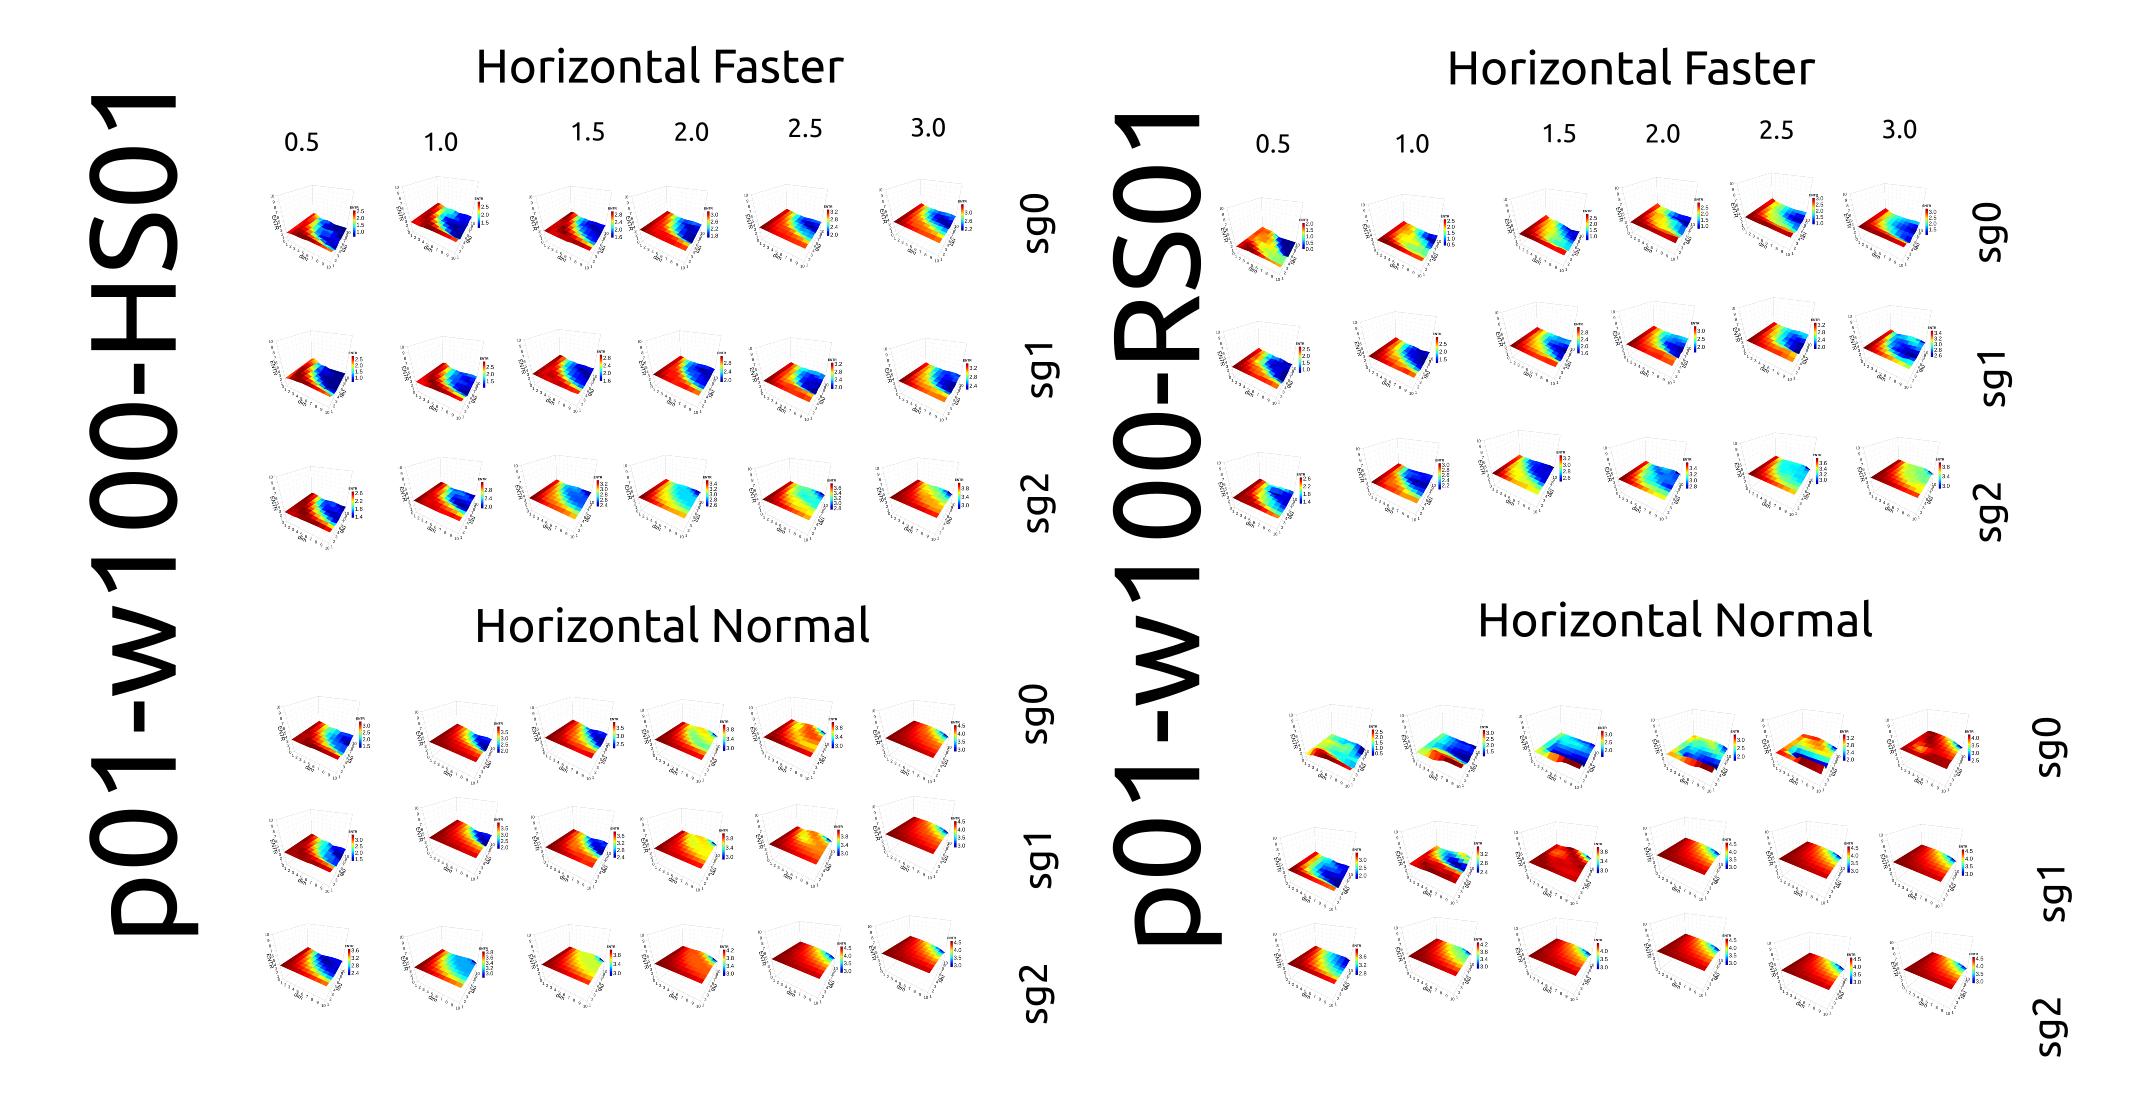
\includegraphics[scale=1.0]{figures/rqa/output/epsilons/rqa-epsilonsp01w100Horizontal}
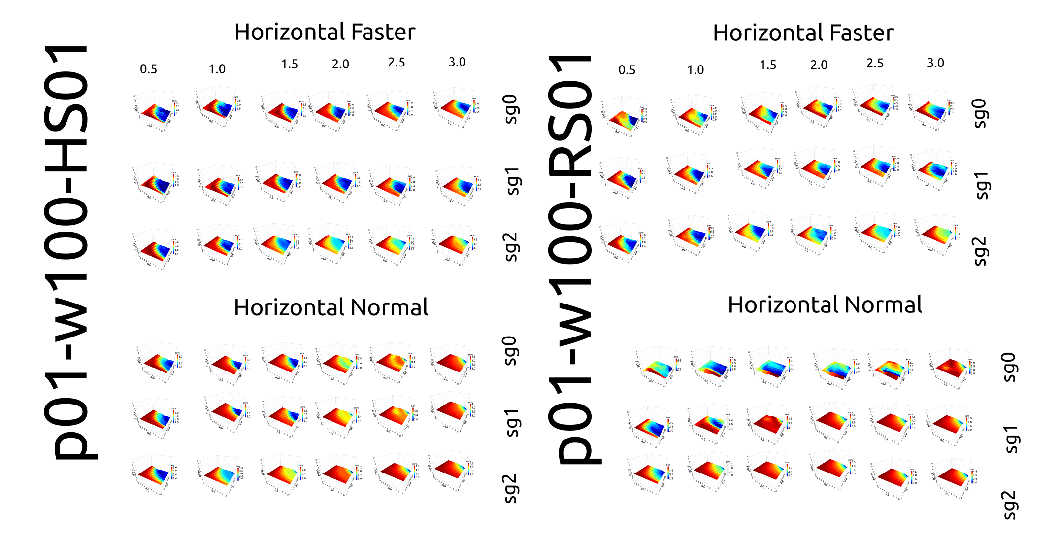
\includegraphics[scale=1.0]{sm-fig01}
    	\caption{
	{\bf RQA-Entr for participant 01 performing horizontal movements for a window size of 100 samples.}
		%RQA-Entr surface plots are for participant $p01$
		%for horizontal and vertical arm movements in normal
		%and faster velocity (HN, HF, VN, VF)
		%with the normalised GyroZ or GyroY axis
		%((sg0) raw-normalised (sg0zmuv),
		%(sg1) normalised-smoothed 1 and
		%(sg1) normalised-smoothed 2)
		%and with one sensor attached to the participant (HS01)
		%and other sensor attached to the robot (RS01).
	Code and data to reproduce the figure is available in \cite{srep2021}.
        }
    \label{fig-p01-H-w100}
\end{figure}
%---------------------------------(FIGURE)------------------------------------
%---------------------------------FIGURE)-------------------------------------
\begin{figure}[hb!]
\centering
%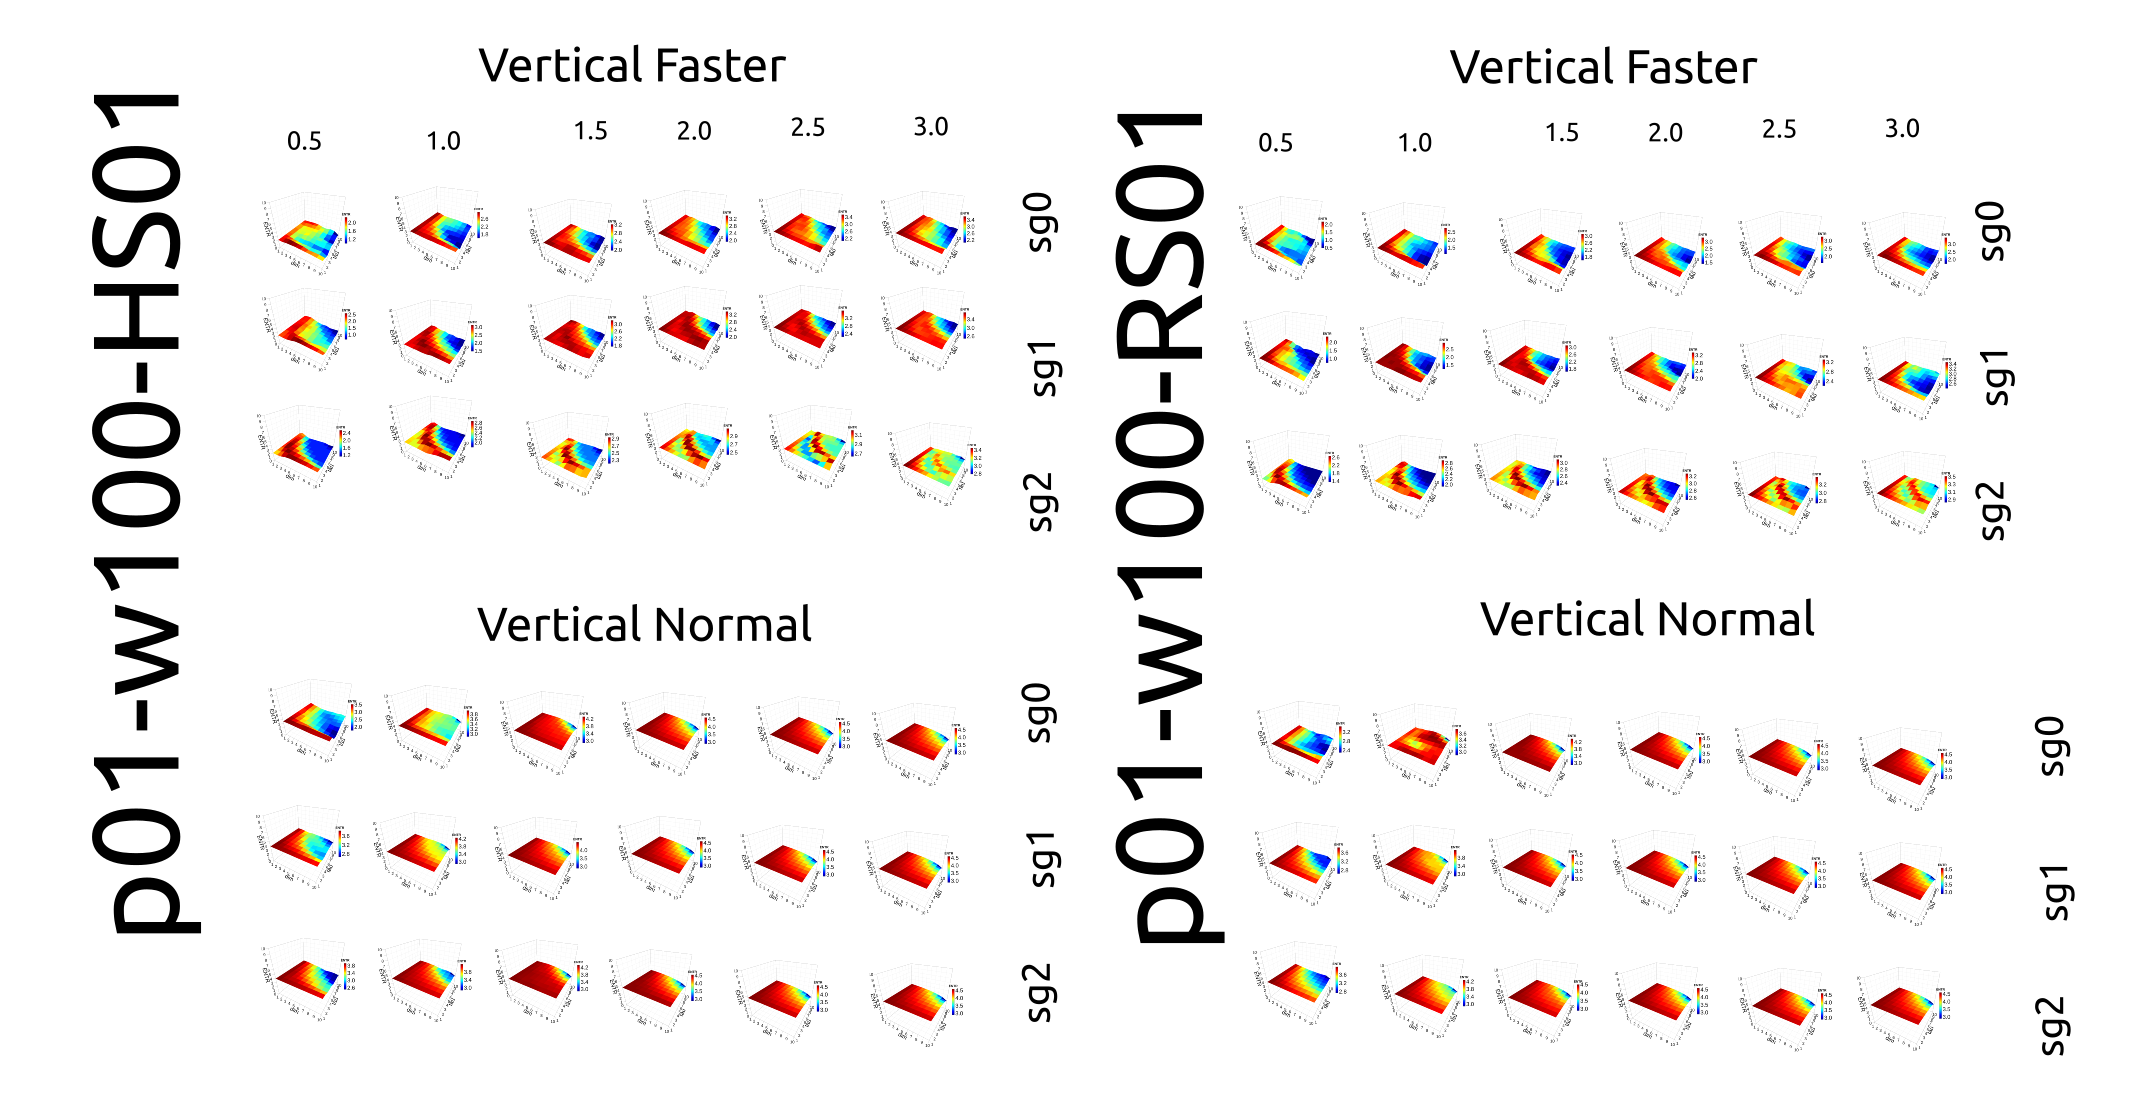
\includegraphics[scale=1.0]{figures/rqa/output/epsilons/rqa-epsilonsp01w100Vertical}
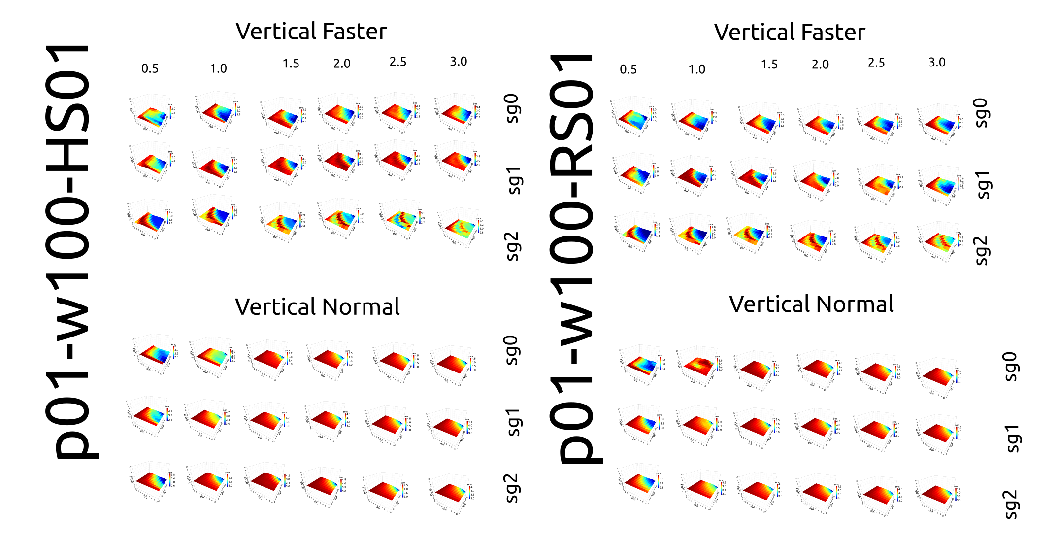
\includegraphics[scale=1.0]{sm-fig02}
    	\caption{
	{\bf RQA-Entr for participant 01 performing vertical movements for a window size of 100 samples.}
		%RQA-Entr surface plots are for participant $p01$
		%for horizontal and vertical arm movements in normal
		%and faster velocity (HN, HF, VN, VF)
		%with the normalised GyroZ or GyroY axis
		%((sg0) raw-normalised (sg0zmuv),
		%(sg1) normalised-smoothed 1 and
		%(sg1) normalised-smoothed 2)
		%and with one sensor attached to the participant (HS01)
		%and other sensor attached to the robot (RS01).
	Code and data to reproduce the figure is available in \cite{srep2021}.
        }
    \label{fig-p01-V-w100}
\end{figure}
%---------------------------------(FIGURE)------------------------------------


\newpage
%---------------------------------FIGURE)-------------------------------------
\begin{figure}[ht!]
\centering
%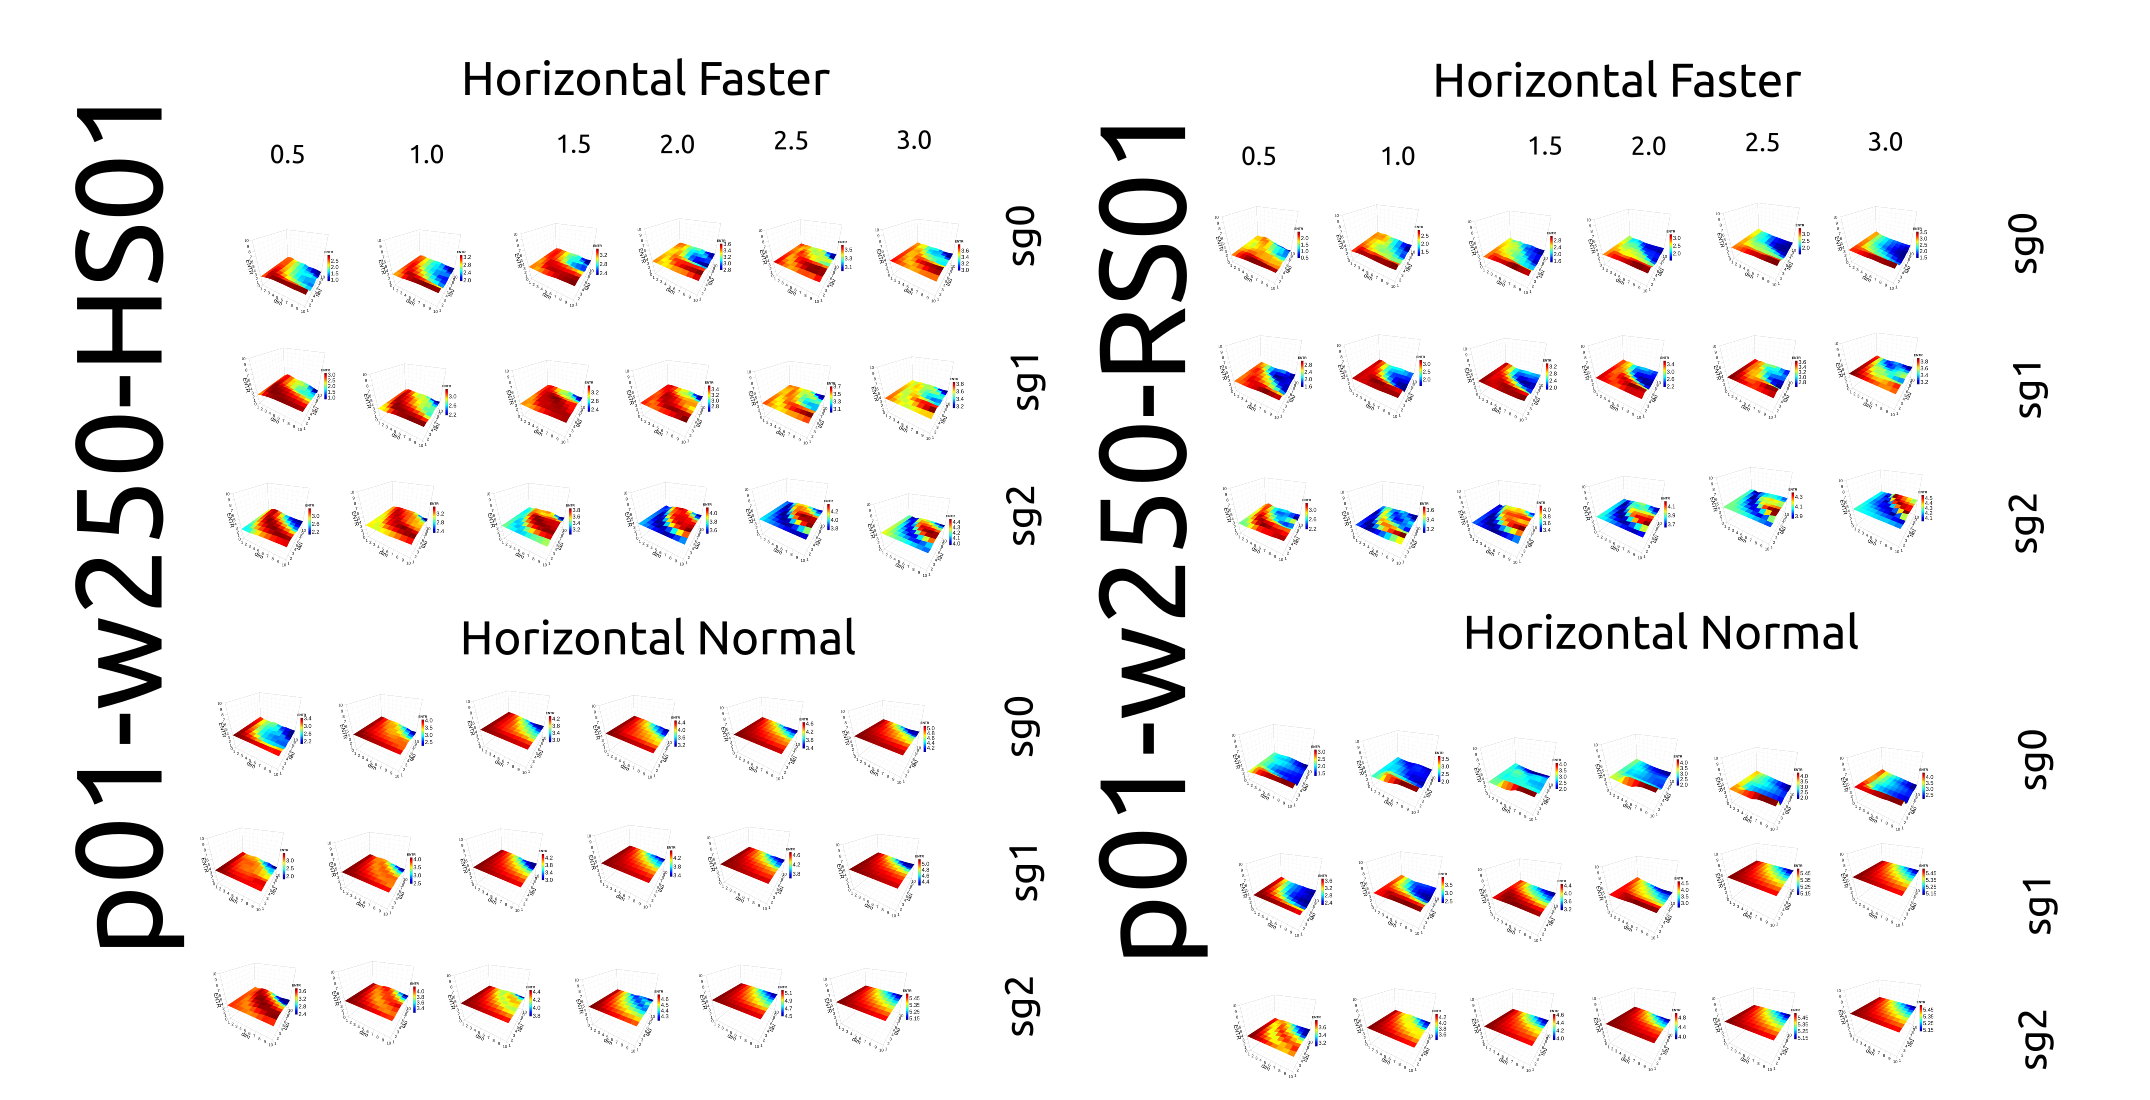
\includegraphics{figures/rqa/output/epsilons/rqa-epsilonsp01w250Horizontal}
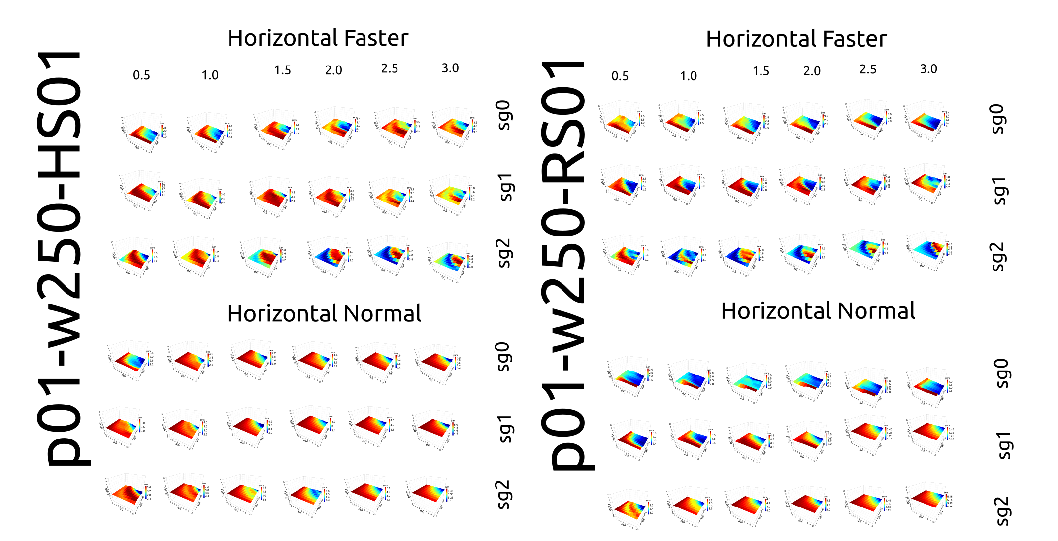
\includegraphics{sm-fig03}
    	\caption{
	{\bf RQA-Entr for participant 01 performing horizontal movements for a window size of 250 samples.}
		%RQA-Entr surface plots are for participant $p01$
		%for horizontal and vertical arm movements in normal
		%and faster velocity (HN, HF, VN, VF)
		%with the normalised GyroZ or GyroY axis
		%((sg0) raw-normalised (sg0zmuv),
		%(sg1) normalised-smoothed 1 and
		%(sg1) normalised-smoothed 2)
		%and with one sensor attached to the participant (HS01)
		%and other sensor attached to the robot (RS01).
	Code and data to reproduce the figure is available in \cite{srep2021}.
        }
    \label{fig-p01-H-w250}
\end{figure}
%---------------------------------(FIGURE)------------------------------------
%---------------------------------FIGURE)-------------------------------------
\begin{figure}[hb!]
\centering
%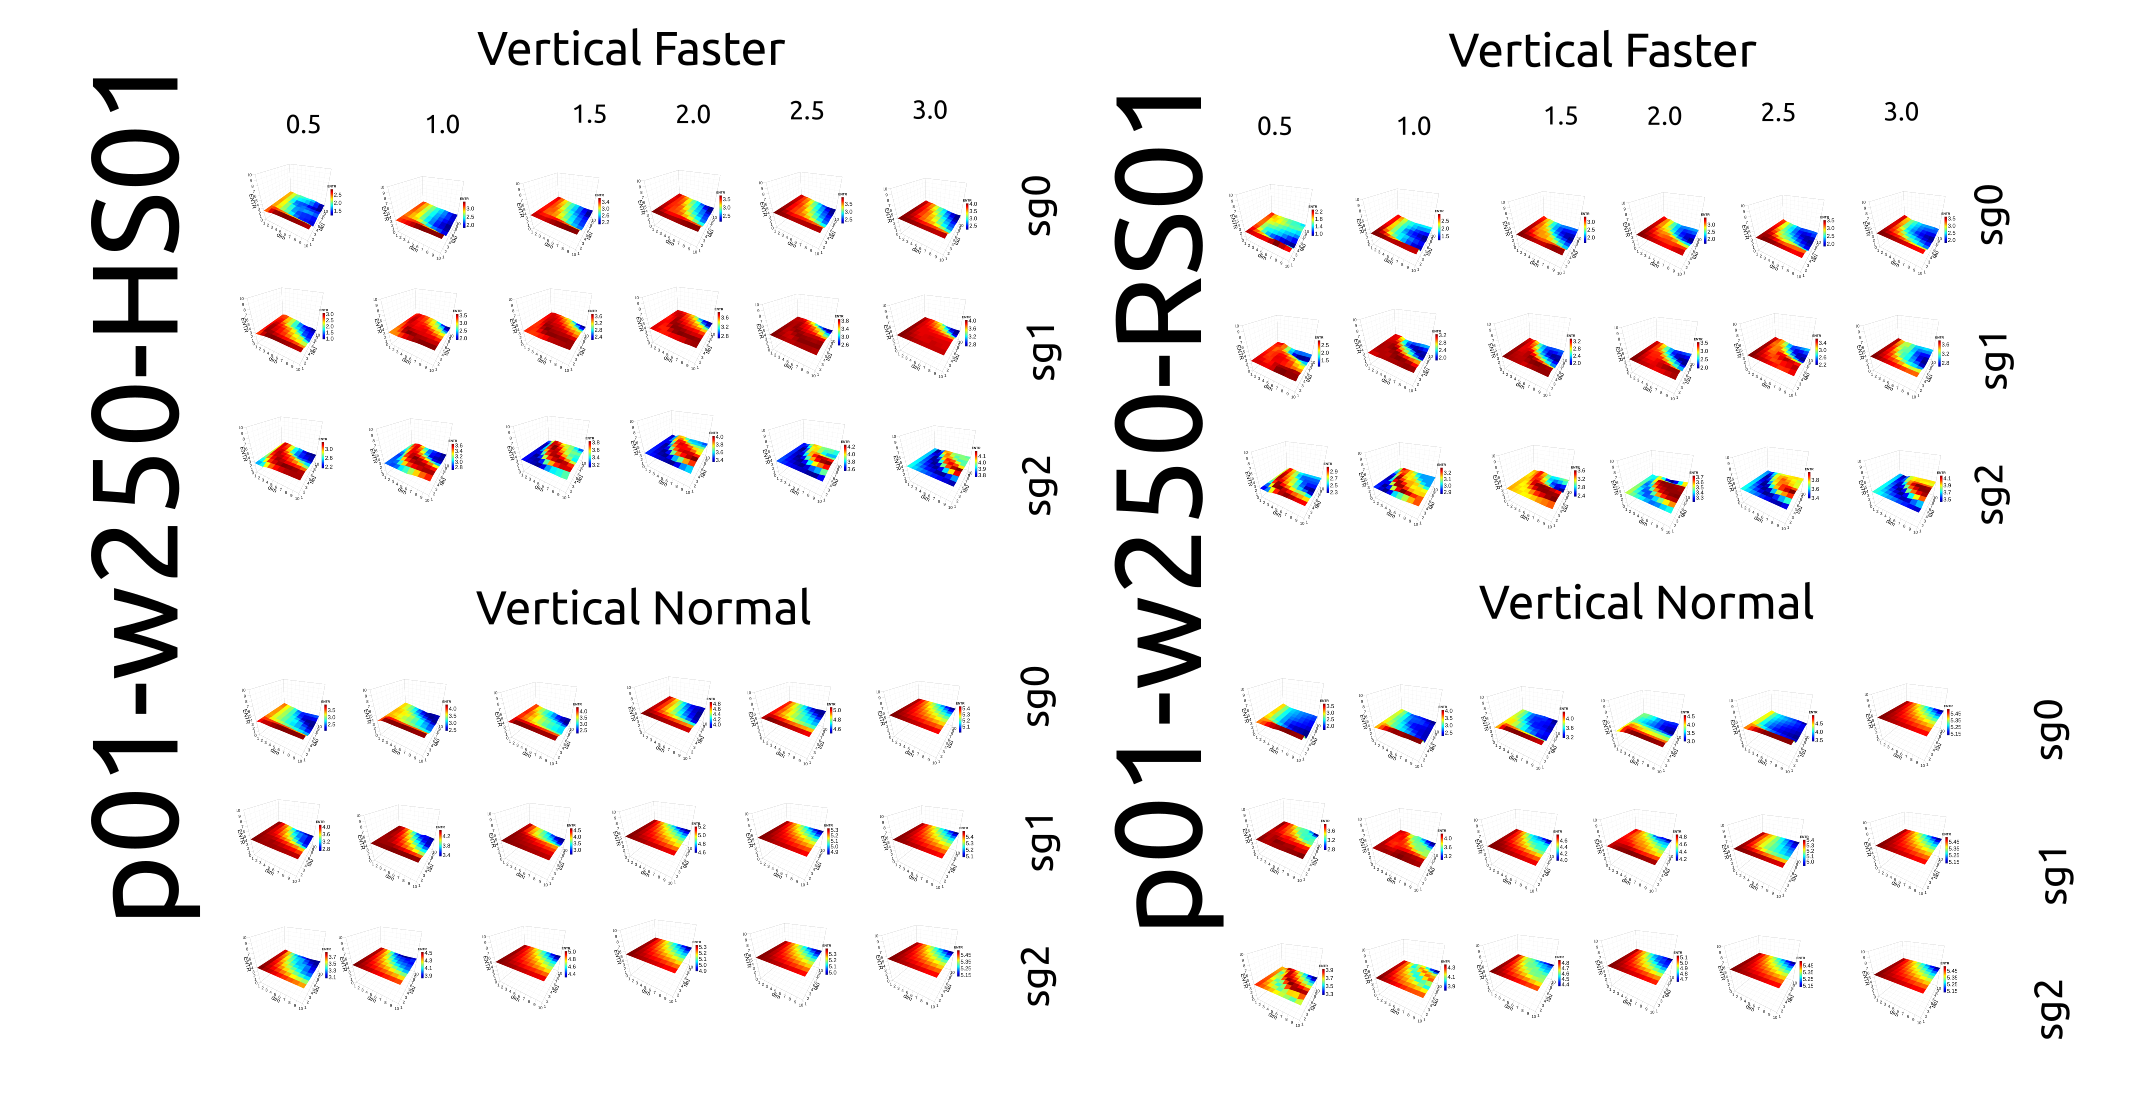
\includegraphics{figures/rqa/output/epsilons/rqa-epsilonsp01w250Vertical}
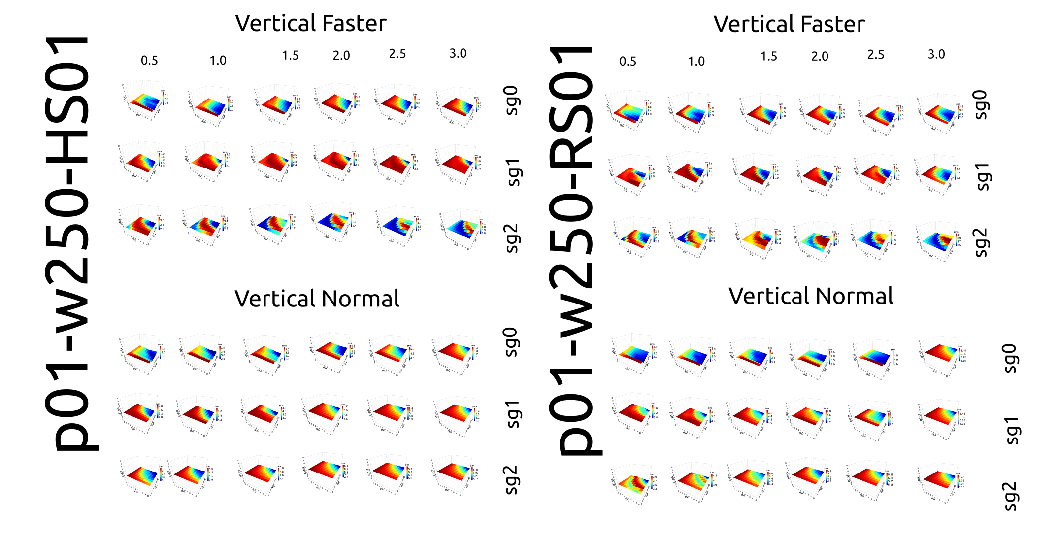
\includegraphics{sm-fig04}
    	\caption{
	{\bf RQA-Entr for participant 01 performing vertical movements for a window size of 250 samples.}
		%RQA-Entr surface plots are for participant $p01$
		%for horizontal and vertical arm movements in normal
		%and faster velocity (HN, HF, VN, VF)
		%with the normalised GyroZ or GyroY axis
		%((sg0) raw-normalised (sg0zmuv),
		%(sg1) normalised-smoothed 1 and
		%(sg1) normalised-smoothed 2)
		%and with one sensor attached to the participant (HS01)
		%and other sensor attached to the robot (RS01).
	Code and data to reproduce the figure is available in \cite{srep2021}.
        }
    \label{fig-p01-V-w250}
\end{figure}
%---------------------------------(FIGURE)------------------------------------


\newpage
%---------------------------------FIGURE)-------------------------------------
\begin{figure}[ht!]
\centering
%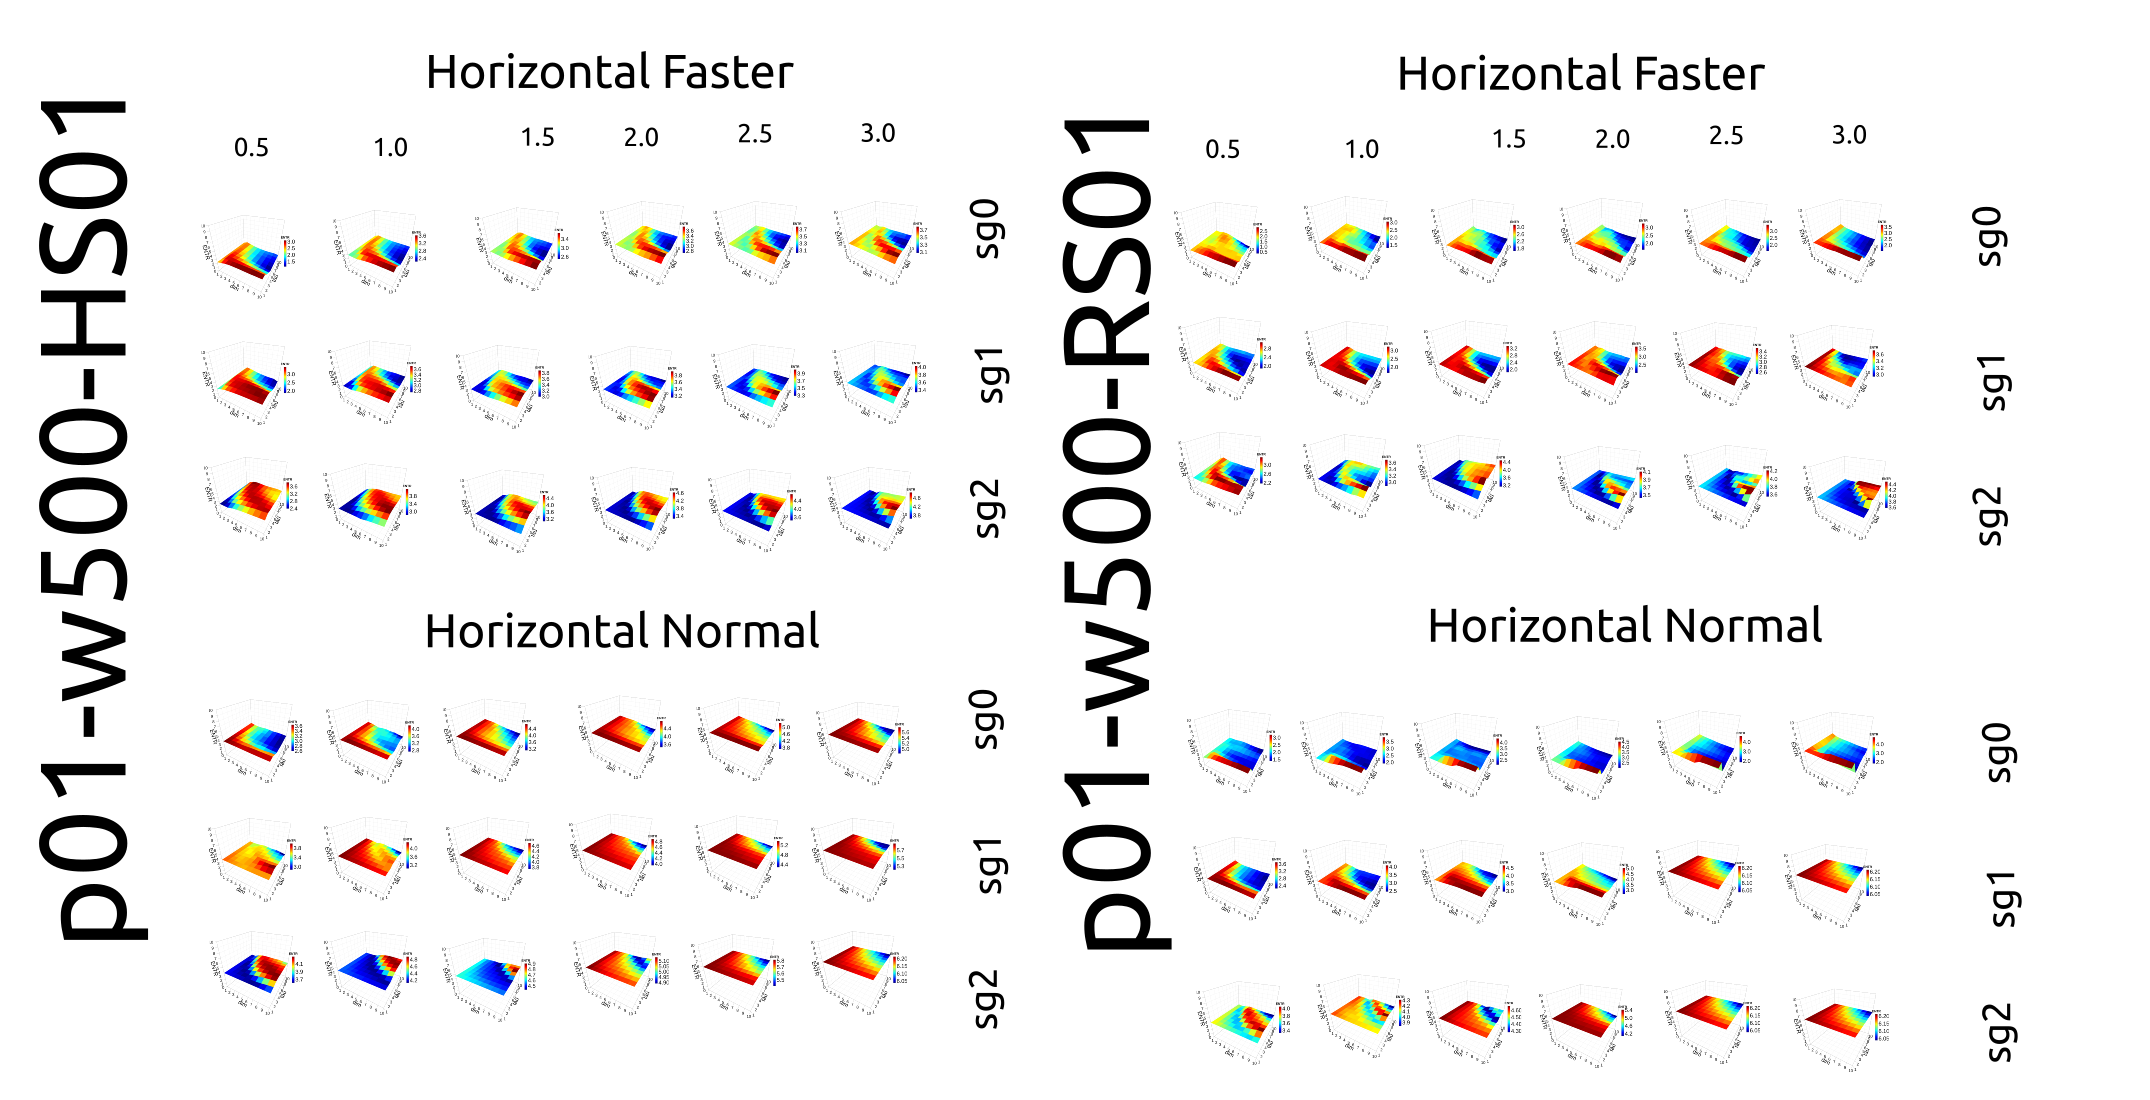
\includegraphics{figures/rqa/output/epsilons/rqa-epsilonsp01w500Horizontal}
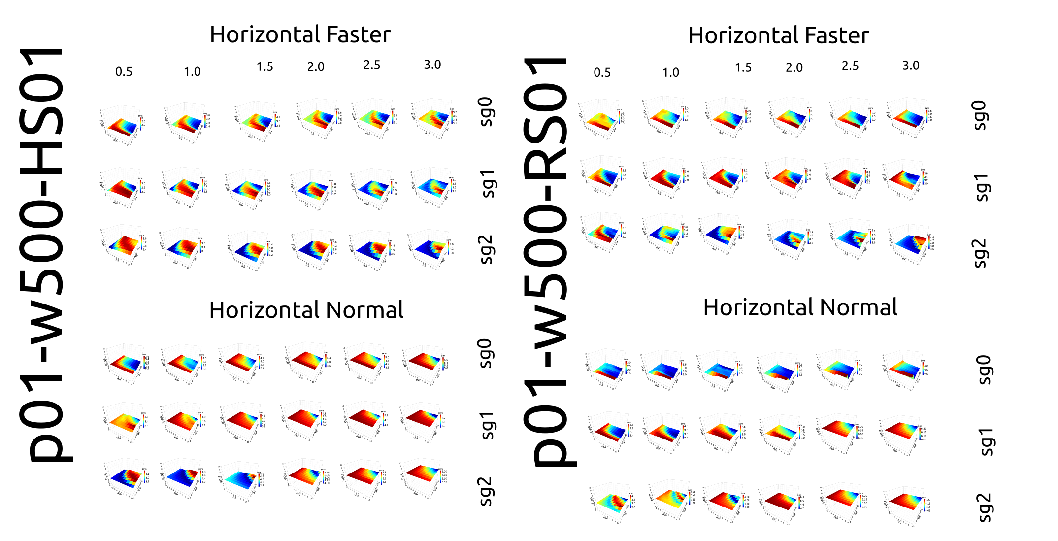
\includegraphics{sm-fig05}
    	\caption{
	{\bf RQA-Entr for participant 01 performing horizontal movements for a window size of 500 samples.}
		%RQA-Entr surface plots are for participant $p01$
		%for horizontal and vertical arm movements in normal
		%and faster velocity (HN, HF, VN, VF)
		%with the normalised GyroZ or GyroY axis
		%((sg0) raw-normalised (sg0zmuv),
		%(sg1) normalised-smoothed 1 and
		%(sg1) normalised-smoothed 2)
		%and with one sensor attached to the participant (HS01)
		%and other sensor attached to the robot (RS01).
	Code and data to reproduce the figure is available in \cite{srep2021}.
        }
    \label{fig-p01-H-w500}
\end{figure}
%---------------------------------(FIGURE)------------------------------------
%---------------------------------FIGURE)-------------------------------------
\begin{figure}[hb!]
\centering
%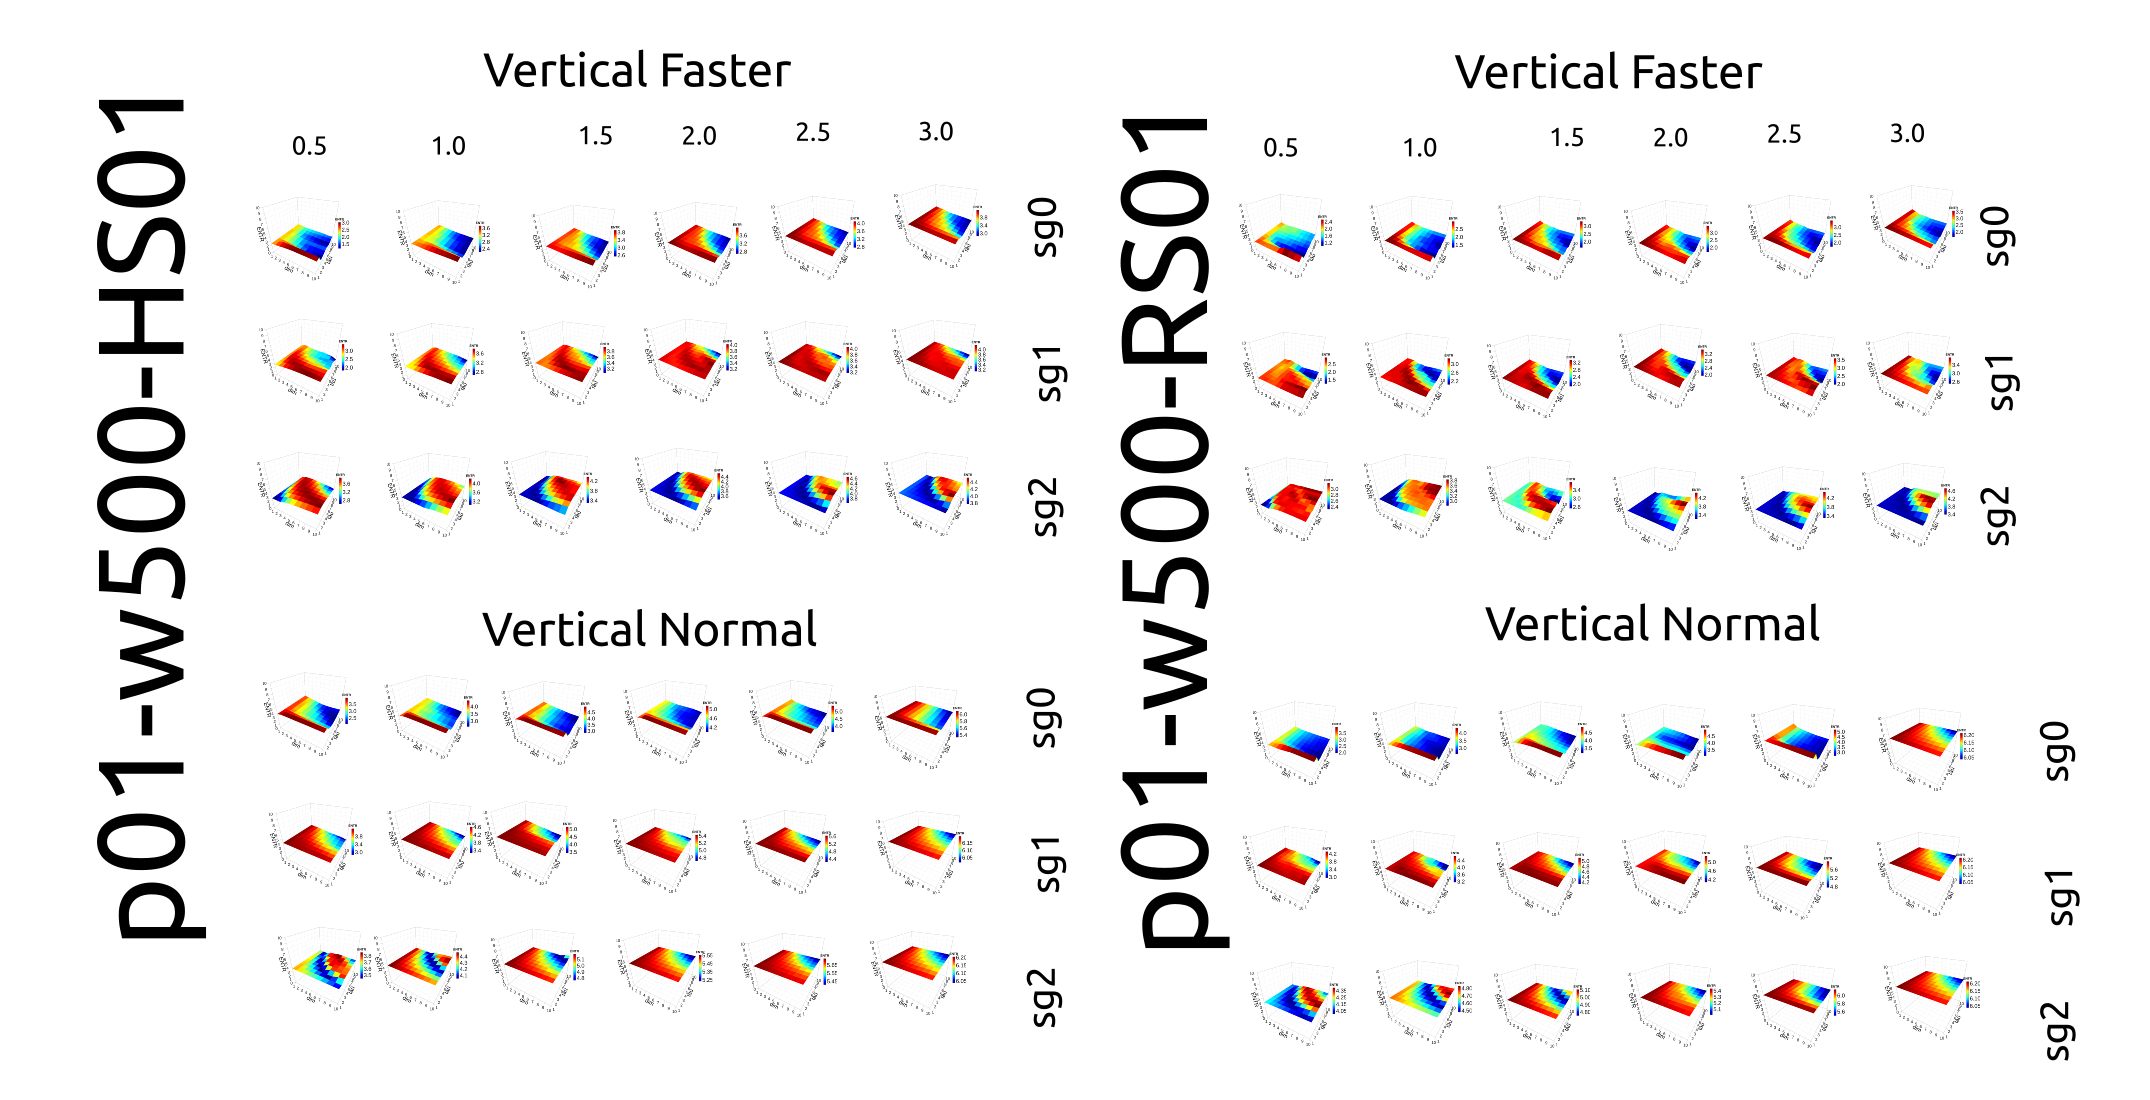
\includegraphics{figures/rqa/output/epsilons/rqa-epsilonsp01w500Vertical}
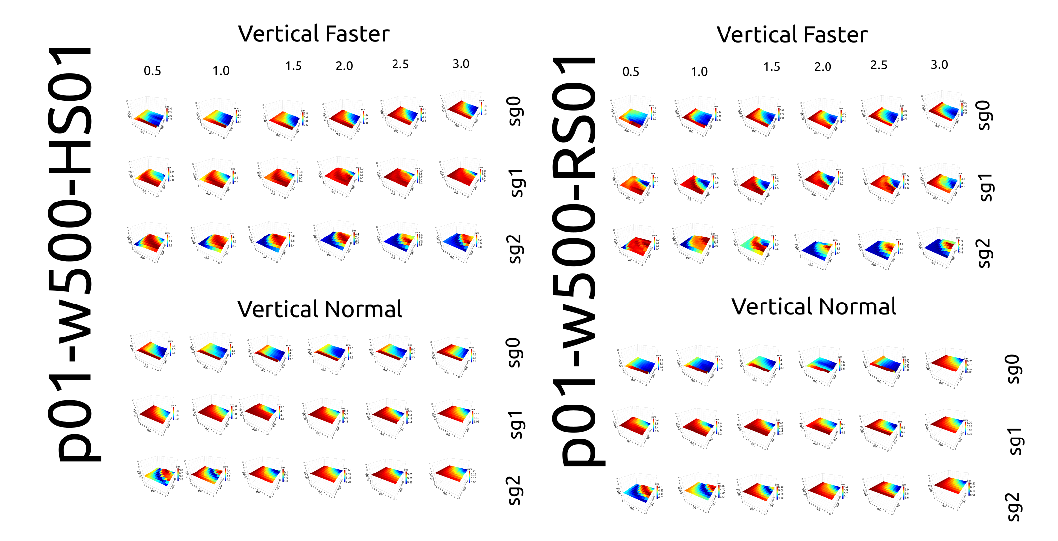
\includegraphics{sm-fig06}
    	\caption{
	{\bf RQA-Entr for participant 01 performing vertical movements for a window size of 500 samples.}
		%RQA-Entr surface plots are for participant $p01$
		%for horizontal and vertical arm movements in normal
		%and faster velocity (HN, HF, VN, VF)
		%with the normalised GyroZ or GyroY axis
		%((sg0) raw-normalised (sg0zmuv),
		%(sg1) normalised-smoothed 1 and
		%(sg1) normalised-smoothed 2)
		%and with one sensor attached to the participant (HS01)
		%and other sensor attached to the robot (RS01).
	Code and data to reproduce the figure is available in \cite{srep2021}.
        }
    \label{fig-p01-V-w500}
\end{figure}
%---------------------------------(FIGURE)------------------------------------


\newpage
%---------------------------------FIGURE)-------------------------------------
\begin{figure}[ht!]
\centering
%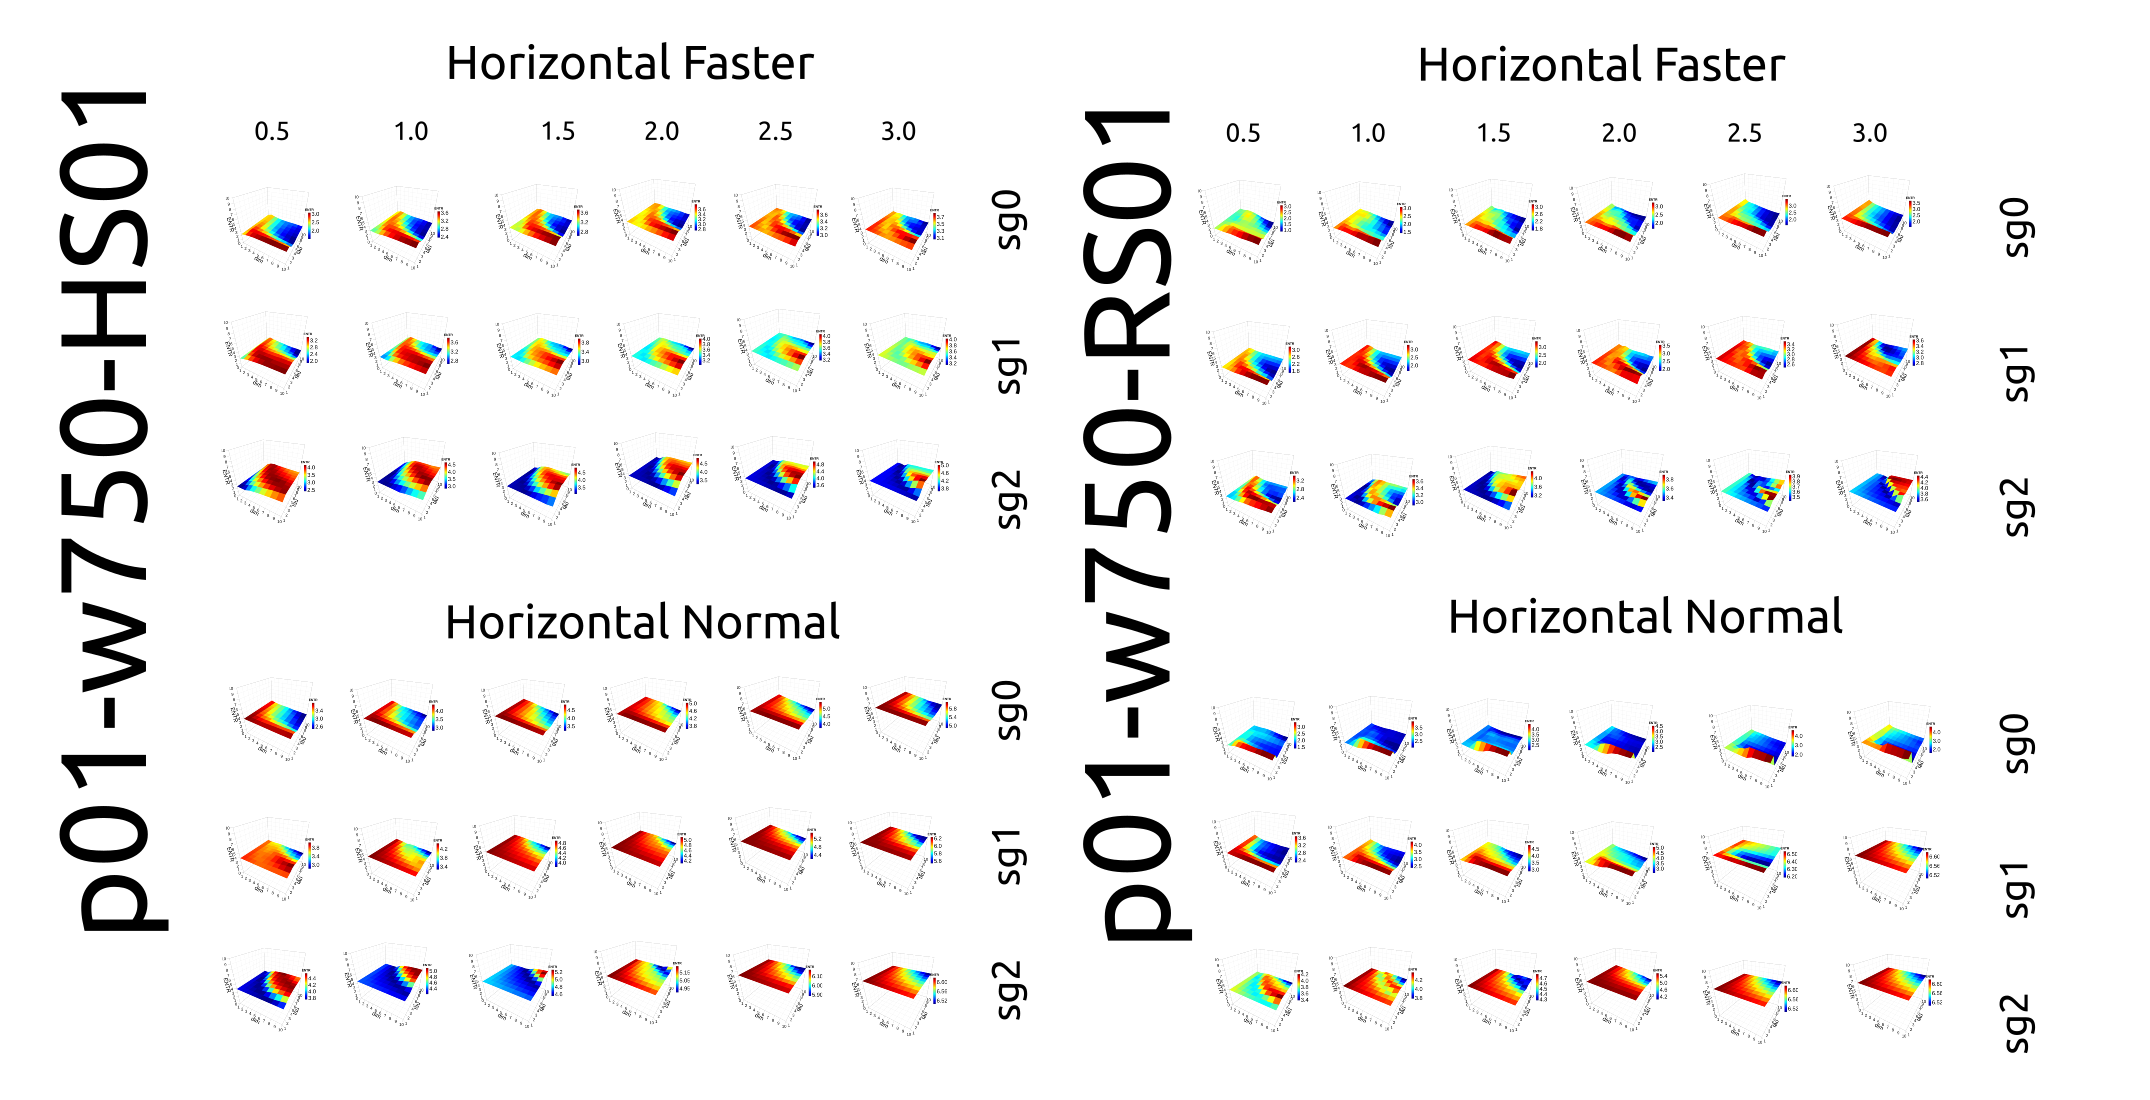
\includegraphics{figures/rqa/output/epsilons/rqa-epsilonsp01w750Horizontal}
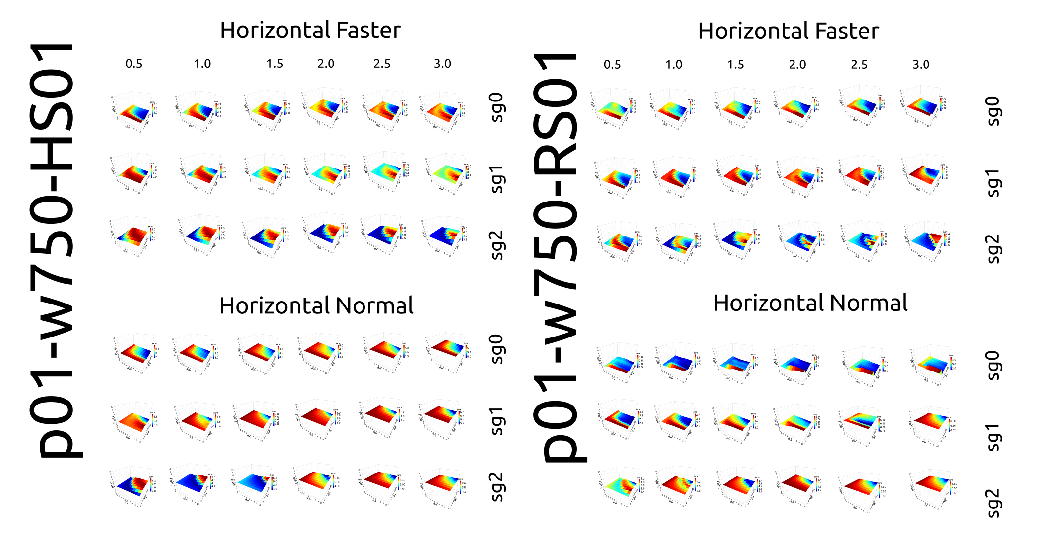
\includegraphics{sm-fig07}
    	\caption{
	{\bf RQA-Entr for participant 01 performing horizontal movements for a window size of 750 samples.}
		%RQA-Entr surface plots are for participant $p01$
		%for horizontal and vertical arm movements in normal
		%and faster velocity (HN, HF, VN, VF)
		%with the normalised GyroZ or GyroY axis
		%((sg0) raw-normalised (sg0zmuv),
		%(sg1) normalised-smoothed 1 and
		%(sg1) normalised-smoothed 2)
		%and with one sensor attached to the participant (HS01)
		%and other sensor attached to the robot (RS01).
	Code and data to reproduce the figure is available in \cite{srep2021}.
        }
    \label{fig-p01-H-w750}
\end{figure}
%---------------------------------(FIGURE)------------------------------------
%---------------------------------FIGURE)-------------------------------------
\begin{figure}[hb!]
\centering
%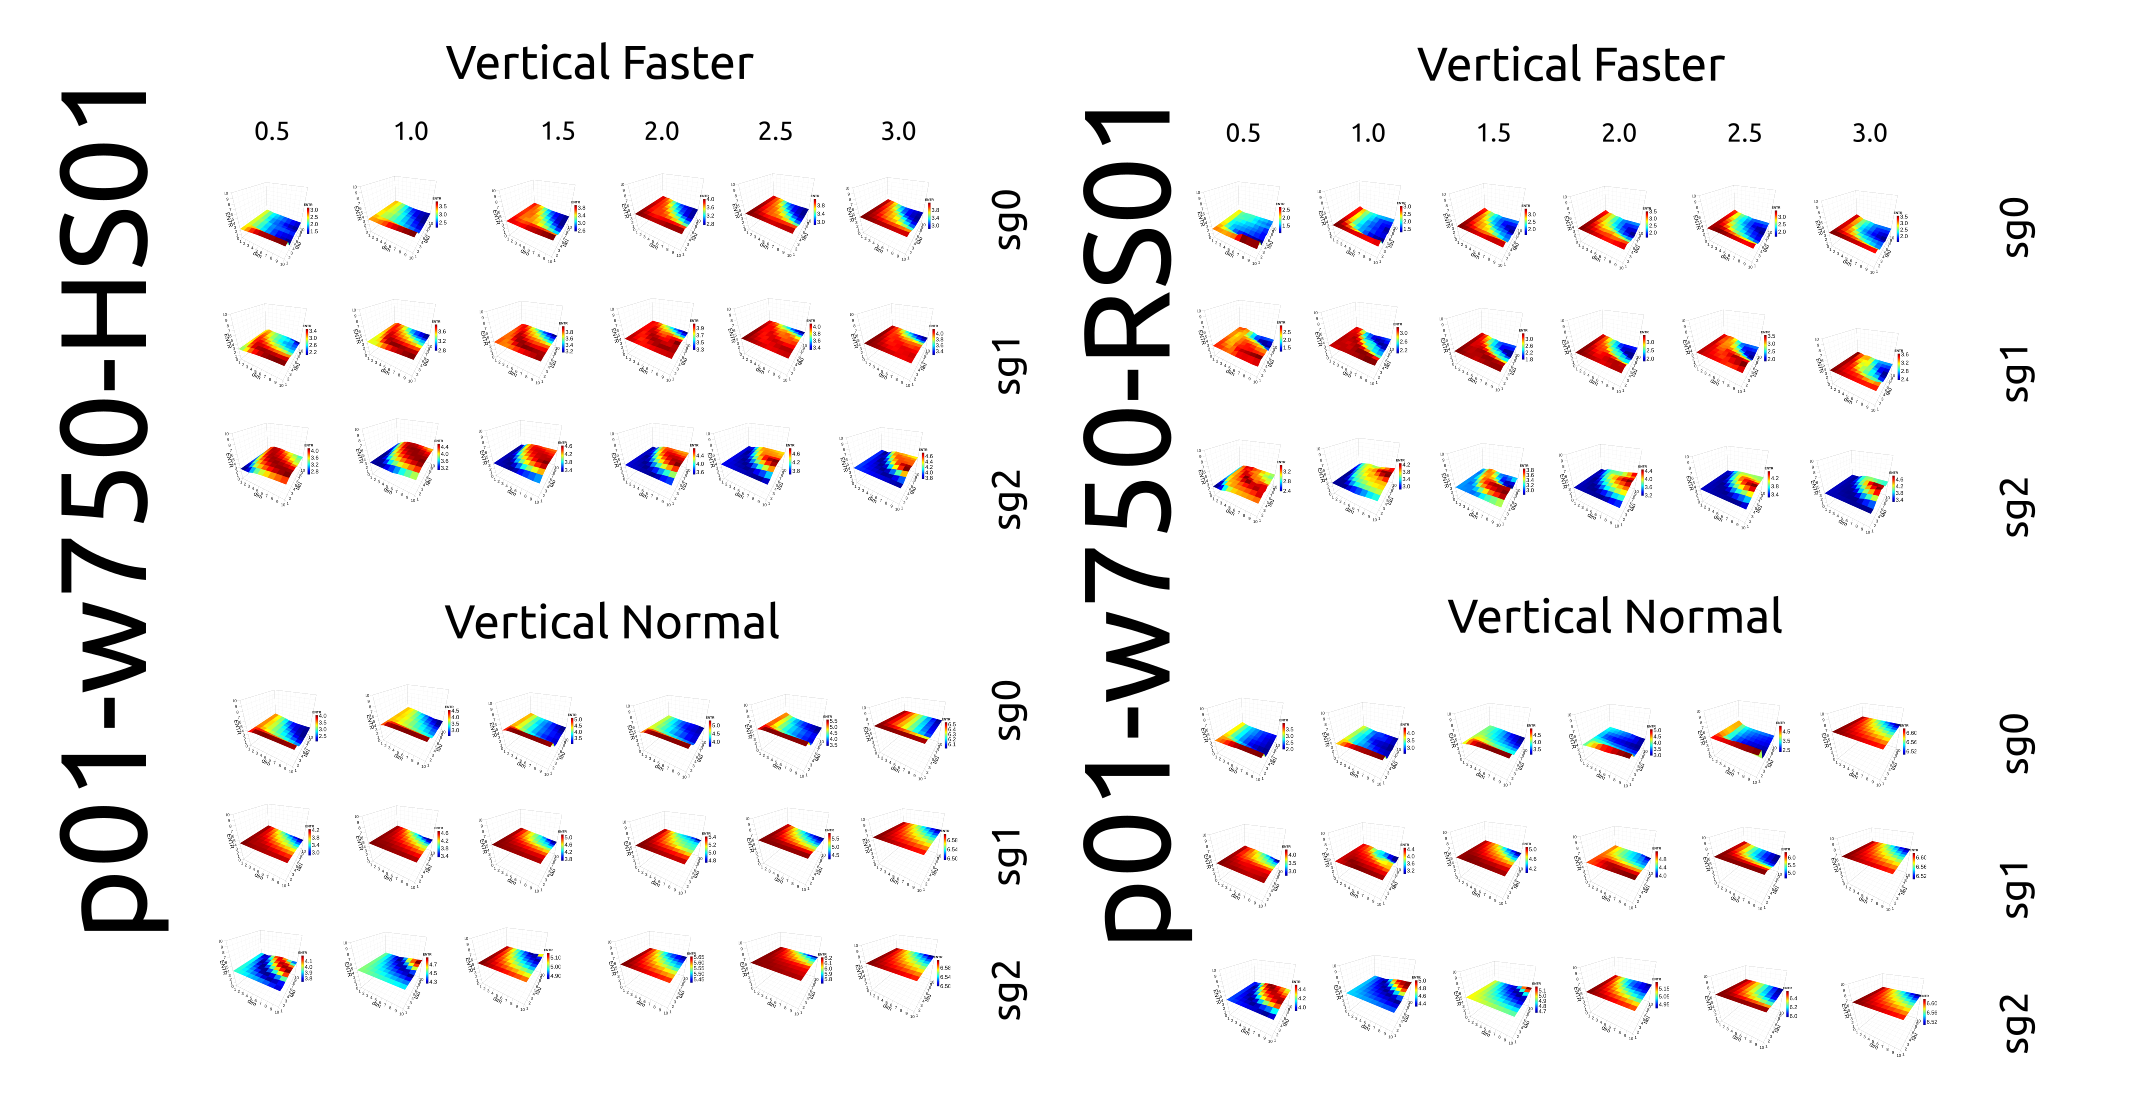
\includegraphics{figures/rqa/output/epsilons/rqa-epsilonsp01w750Vertical}
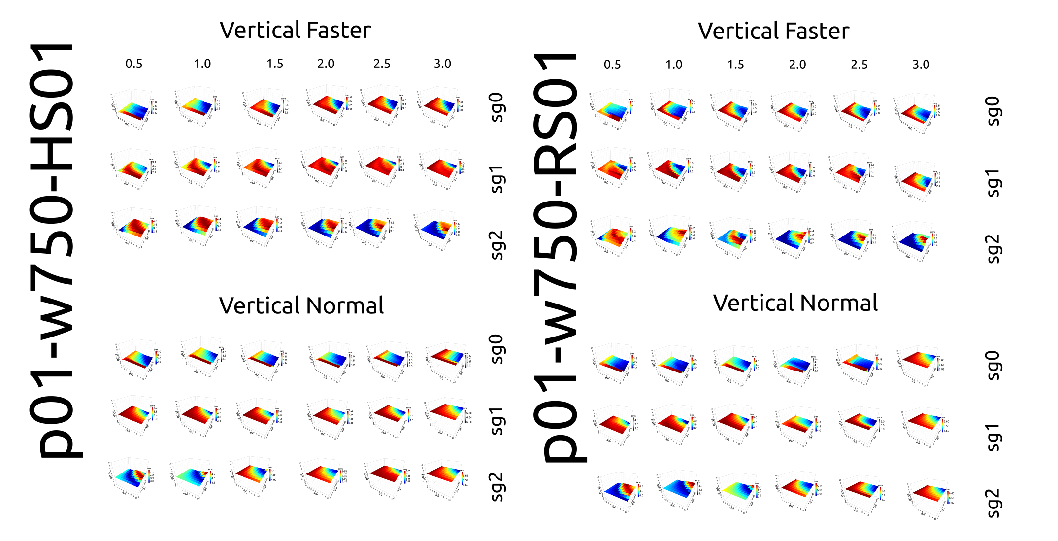
\includegraphics{sm-fig08}
    	\caption{
	{\bf RQA-Entr for participant 01 performing vertical movements for a window size of 750 samples.}
		%RQA-Entr surface plots are for participant $p01$
		%for horizontal and vertical arm movements in normal
		%and faster velocity (HN, HF, VN, VF)
		%with the normalised GyroZ or GyroY axis
		%((sg0) raw-normalised (sg0zmuv),
		%(sg1) normalised-smoothed 1 and
		%(sg1) normalised-smoothed 2)
		%and with one sensor attached to the participant (HS01)
		%and other sensor attached to the robot (RS01).
	Code and data to reproduce the figure is available in \cite{srep2021}.
        }
    \label{fig-p01-V-w750}
\end{figure}
%---------------------------------(FIGURE)------------------------------------






\newpage
\subsection{Participant 02}
%X Three level of
%X smoothness were computed for RQA metrics showing smoothed 3D surfaces and
%X the level of smoothness increase (Fig.~\ref{fig:topo_smoothness}).
%After data collection, raw time series were windowed, normalised and
%smoothed. Then, due to space limitations and to have simple visualisation,
Figures \ref{fig-p02-H-w100} and \ref{fig-p02-V-w100} are for a window size of 100 samples.
Figures \ref{fig-p02-H-w250} and \ref{fig-p02-V-w250} are for a window size of 250 samples.
Figures \ref{fig-p02-H-w500} and \ref{fig-p02-V-w500} are for a window size of 500 samples.
Figures \ref{fig-p02-H-w750} and \ref{fig-p02-V-w750} are for a window size of 750 samples.

\newpage
%---------------------------------FIGURE)-------------------------------------
\begin{figure}[ht!]
\centering
%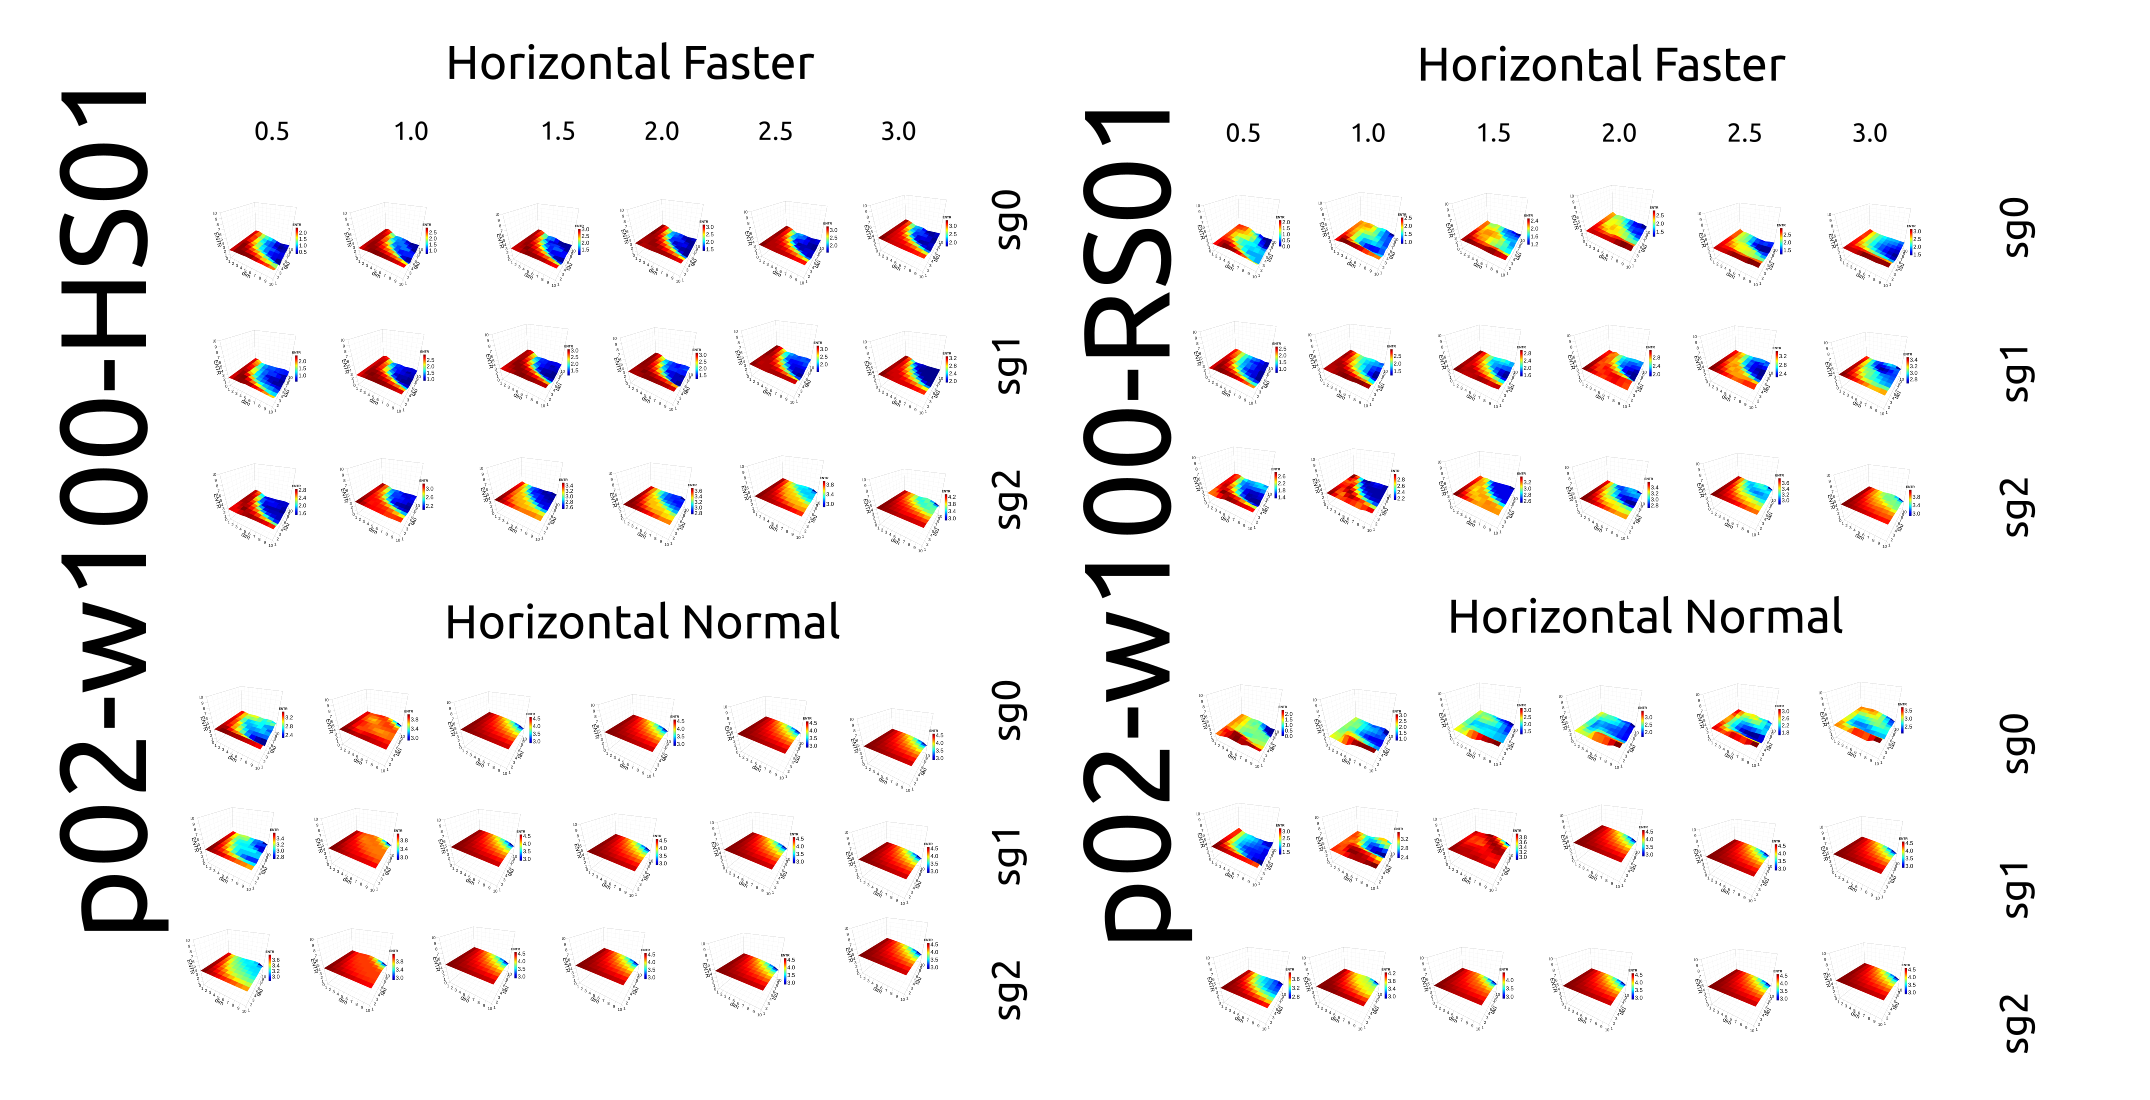
\includegraphics[scale=1.0]{figures/rqa/output/epsilons/rqa-epsilonsp02w100Horizontal}
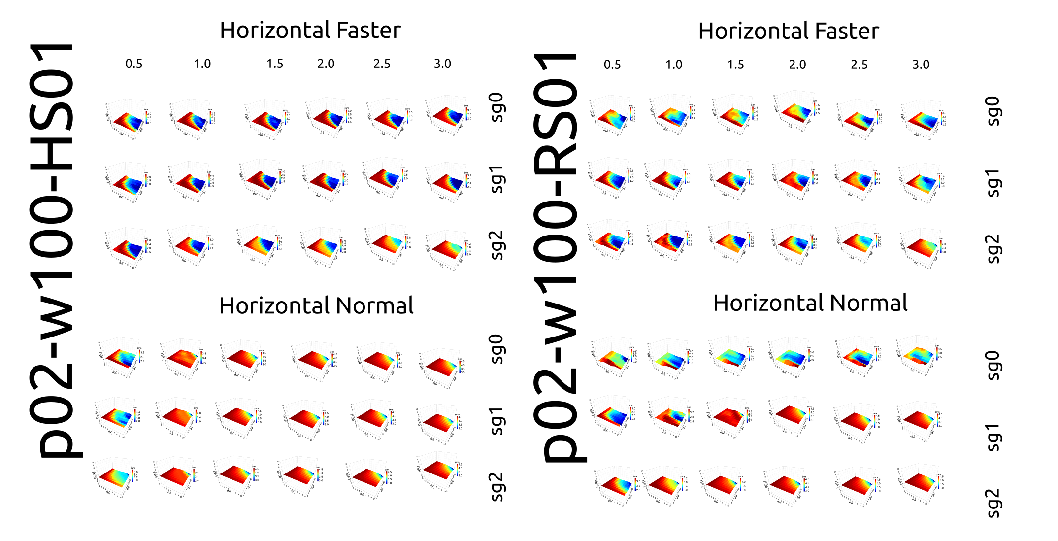
\includegraphics[scale=1.0]{sm-fig09}
    	\caption{
	{\bf RQA-Entr for participant 02 performing horizontal movements for a window size of 100 samples.}
		%RQA-Entr surface plots are for participant $p02$
		%for horizontal and vertical arm movements in normal
		%and faster velocity (HN, HF, VN, VF)
		%with the normalised GyroZ or GyroY axis
		%((sg0) raw-normalised (sg0zmuv),
		%(sg1) normalised-smoothed 1 and
		%(sg1) normalised-smoothed 2)
		%and with one sensor attached to the participant (HS01)
		%and other sensor attached to the robot (RS01).
	Code and data to reproduce the figure is available in \cite{srep2021}.
        }
    \label{fig-p02-H-w100}
\end{figure}
%---------------------------------(FIGURE)------------------------------------
%---------------------------------FIGURE)-------------------------------------
\begin{figure}[hb!]
\centering
%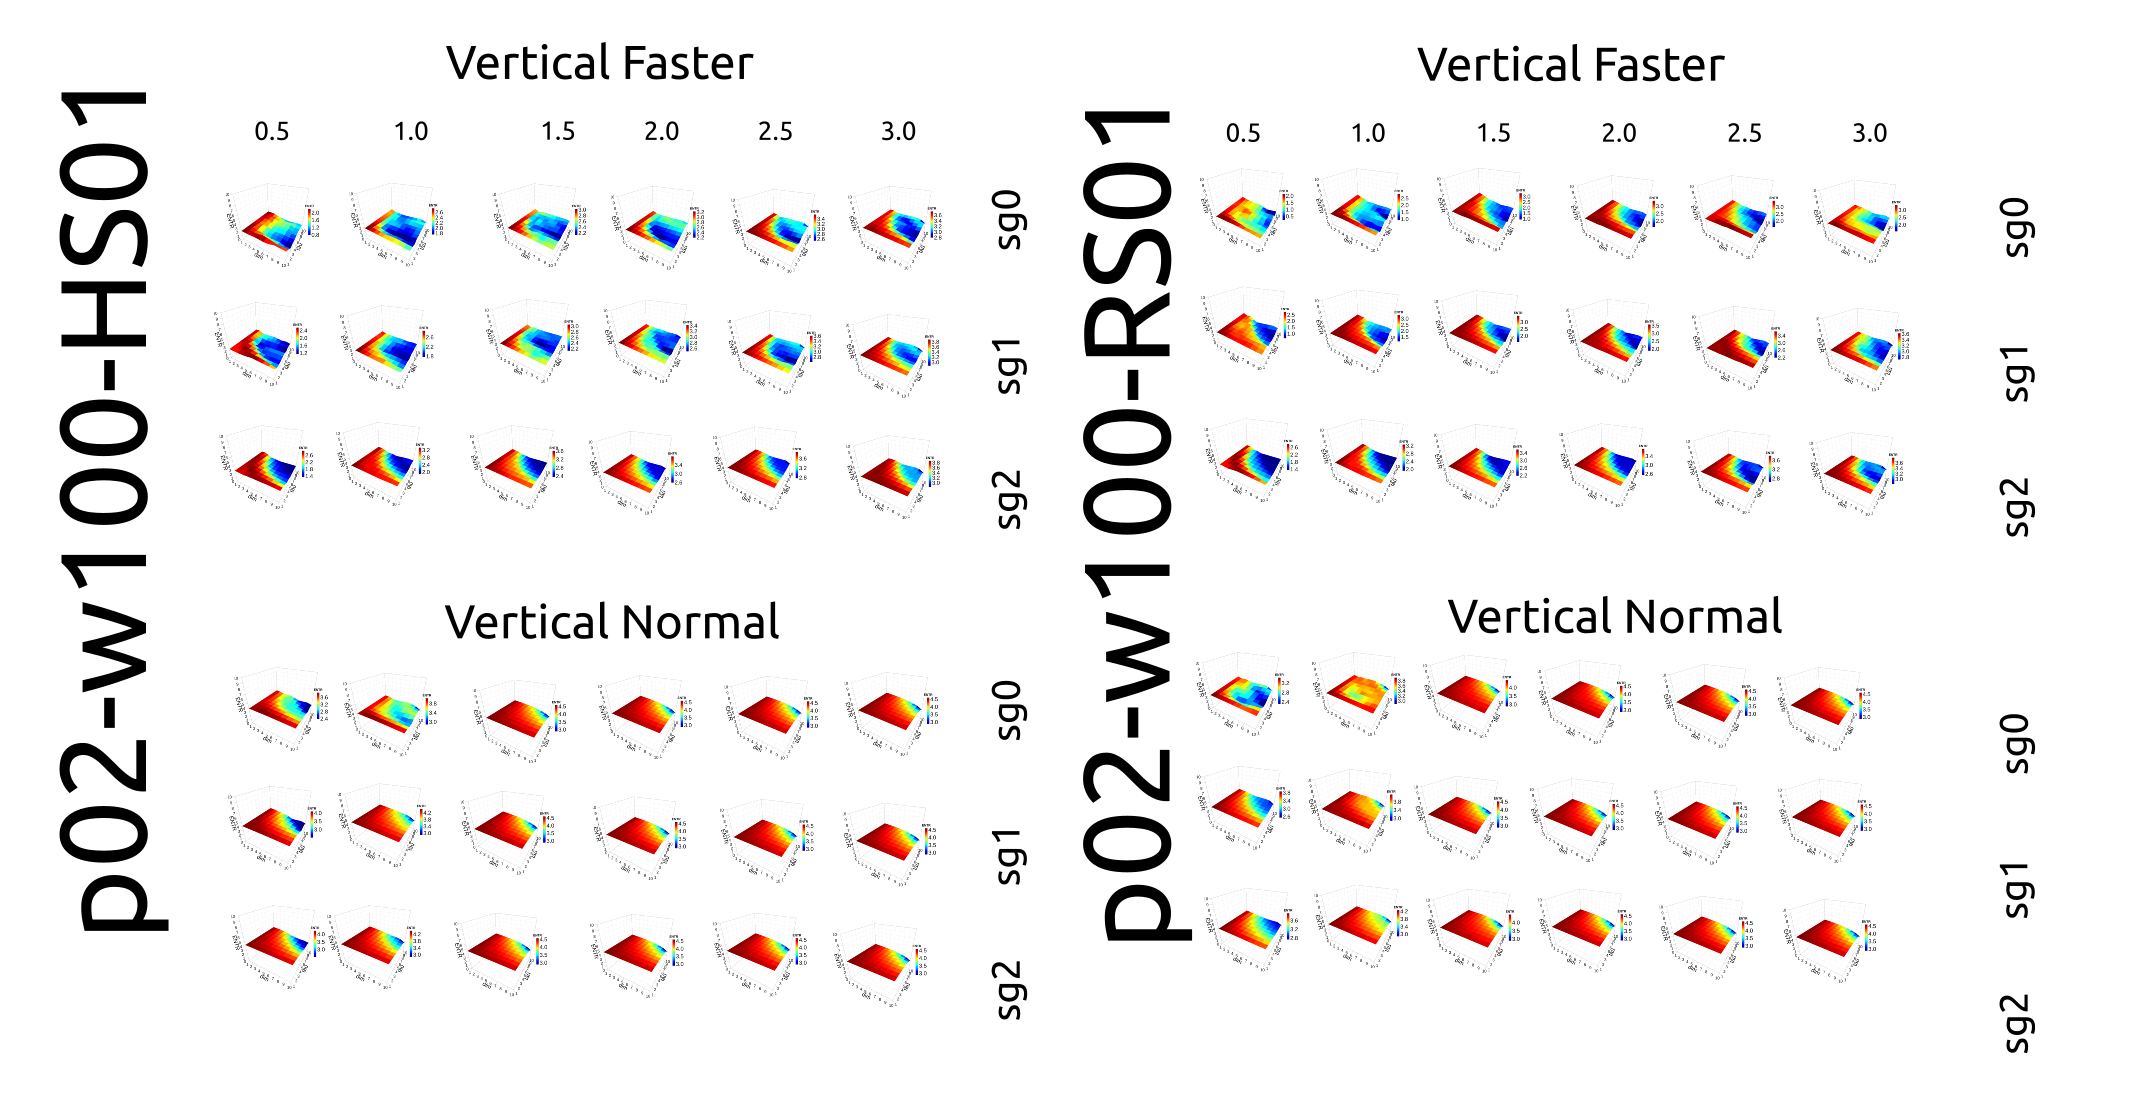
\includegraphics[scale=1.0]{figures/rqa/output/epsilons/rqa-epsilonsp02w100Vertical}
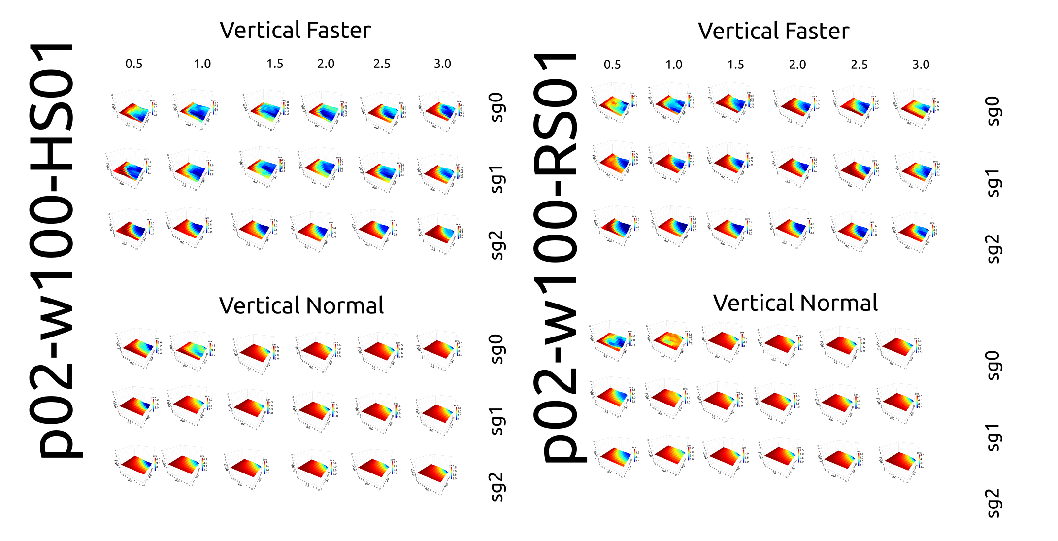
\includegraphics[scale=1.0]{sm-fig10}
    	\caption{
	{\bf RQA-Entr for participant 02 performing vertical movements for a window size of 100 samples.}
		%RQA-Entr surface plots are for participant $p02$
		%for horizontal and vertical arm movements in normal
		%and faster velocity (HN, HF, VN, VF)
		%with the normalised GyroZ or GyroY axis
		%((sg0) raw-normalised (sg0zmuv),
		%(sg1) normalised-smoothed 1 and
		%(sg1) normalised-smoothed 2)
		%and with one sensor attached to the participant (HS01)
		%and other sensor attached to the robot (RS01).
	Code and data to reproduce the figure is available in \cite{srep2021}.
        }
    \label{fig-p02-V-w100}
\end{figure}
%---------------------------------(FIGURE)------------------------------------


\newpage
%---------------------------------FIGURE)-------------------------------------
\begin{figure}[ht!]
\centering
%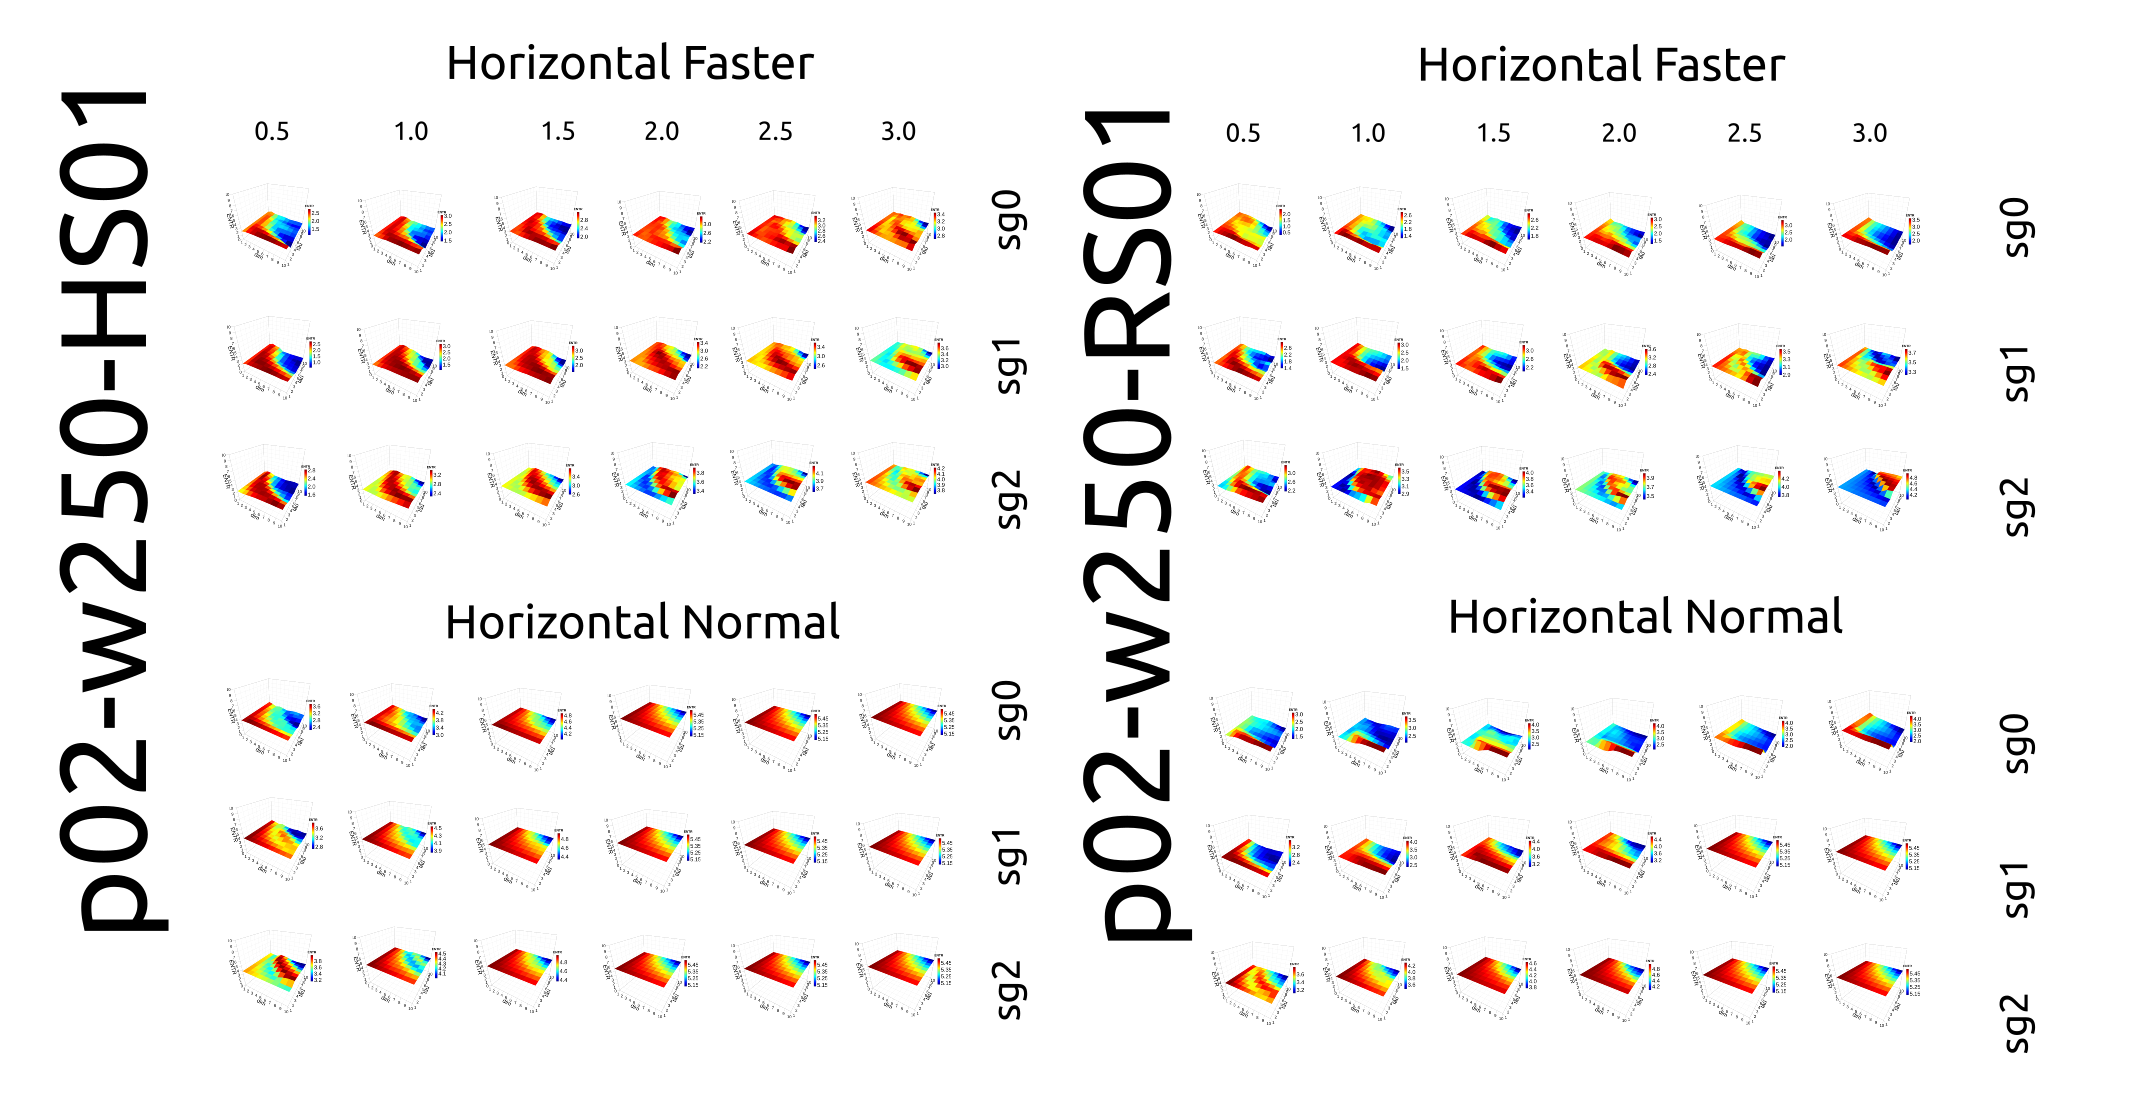
\includegraphics{figures/rqa/output/epsilons/rqa-epsilonsp02w250Horizontal}
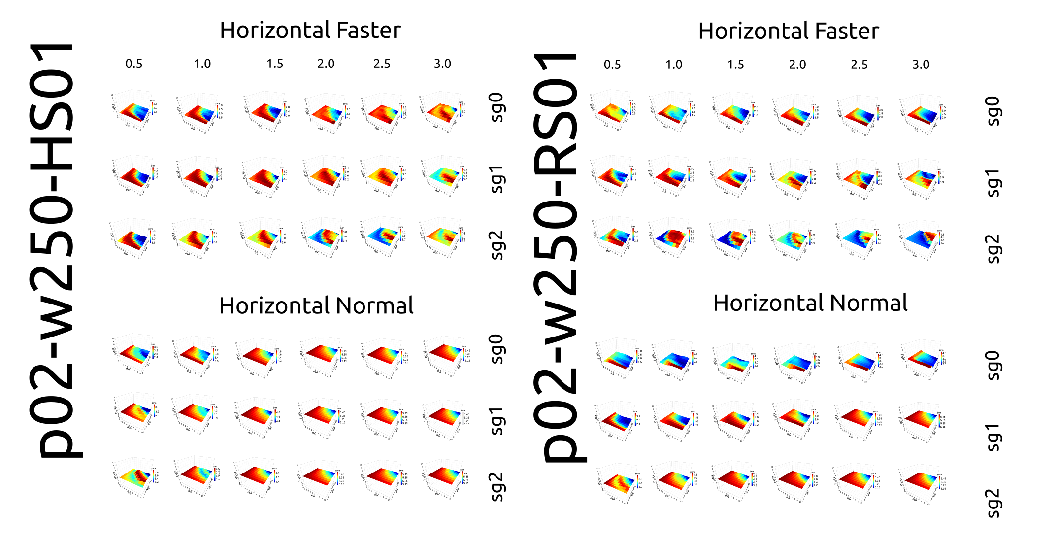
\includegraphics{sm-fig11}
    	\caption{
	{\bf RQA-Entr for participant 02 performing horizontal movements for a window size of 250 samples.}
		%RQA-Entr surface plots are for participant $p02$
		%for horizontal and vertical arm movements in normal
		%and faster velocity (HN, HF, VN, VF)
		%with the normalised GyroZ or GyroY axis
		%((sg0) raw-normalised (sg0zmuv),
		%(sg1) normalised-smoothed 1 and
		%(sg1) normalised-smoothed 2)
		%and with one sensor attached to the participant (HS01)
		%and other sensor attached to the robot (RS01).
	Code and data to reproduce the figure is available in \cite{srep2021}.
        }
    \label{fig-p02-H-w250}
\end{figure}
%---------------------------------(FIGURE)------------------------------------
%---------------------------------FIGURE)-------------------------------------
\begin{figure}[hb!]
\centering
%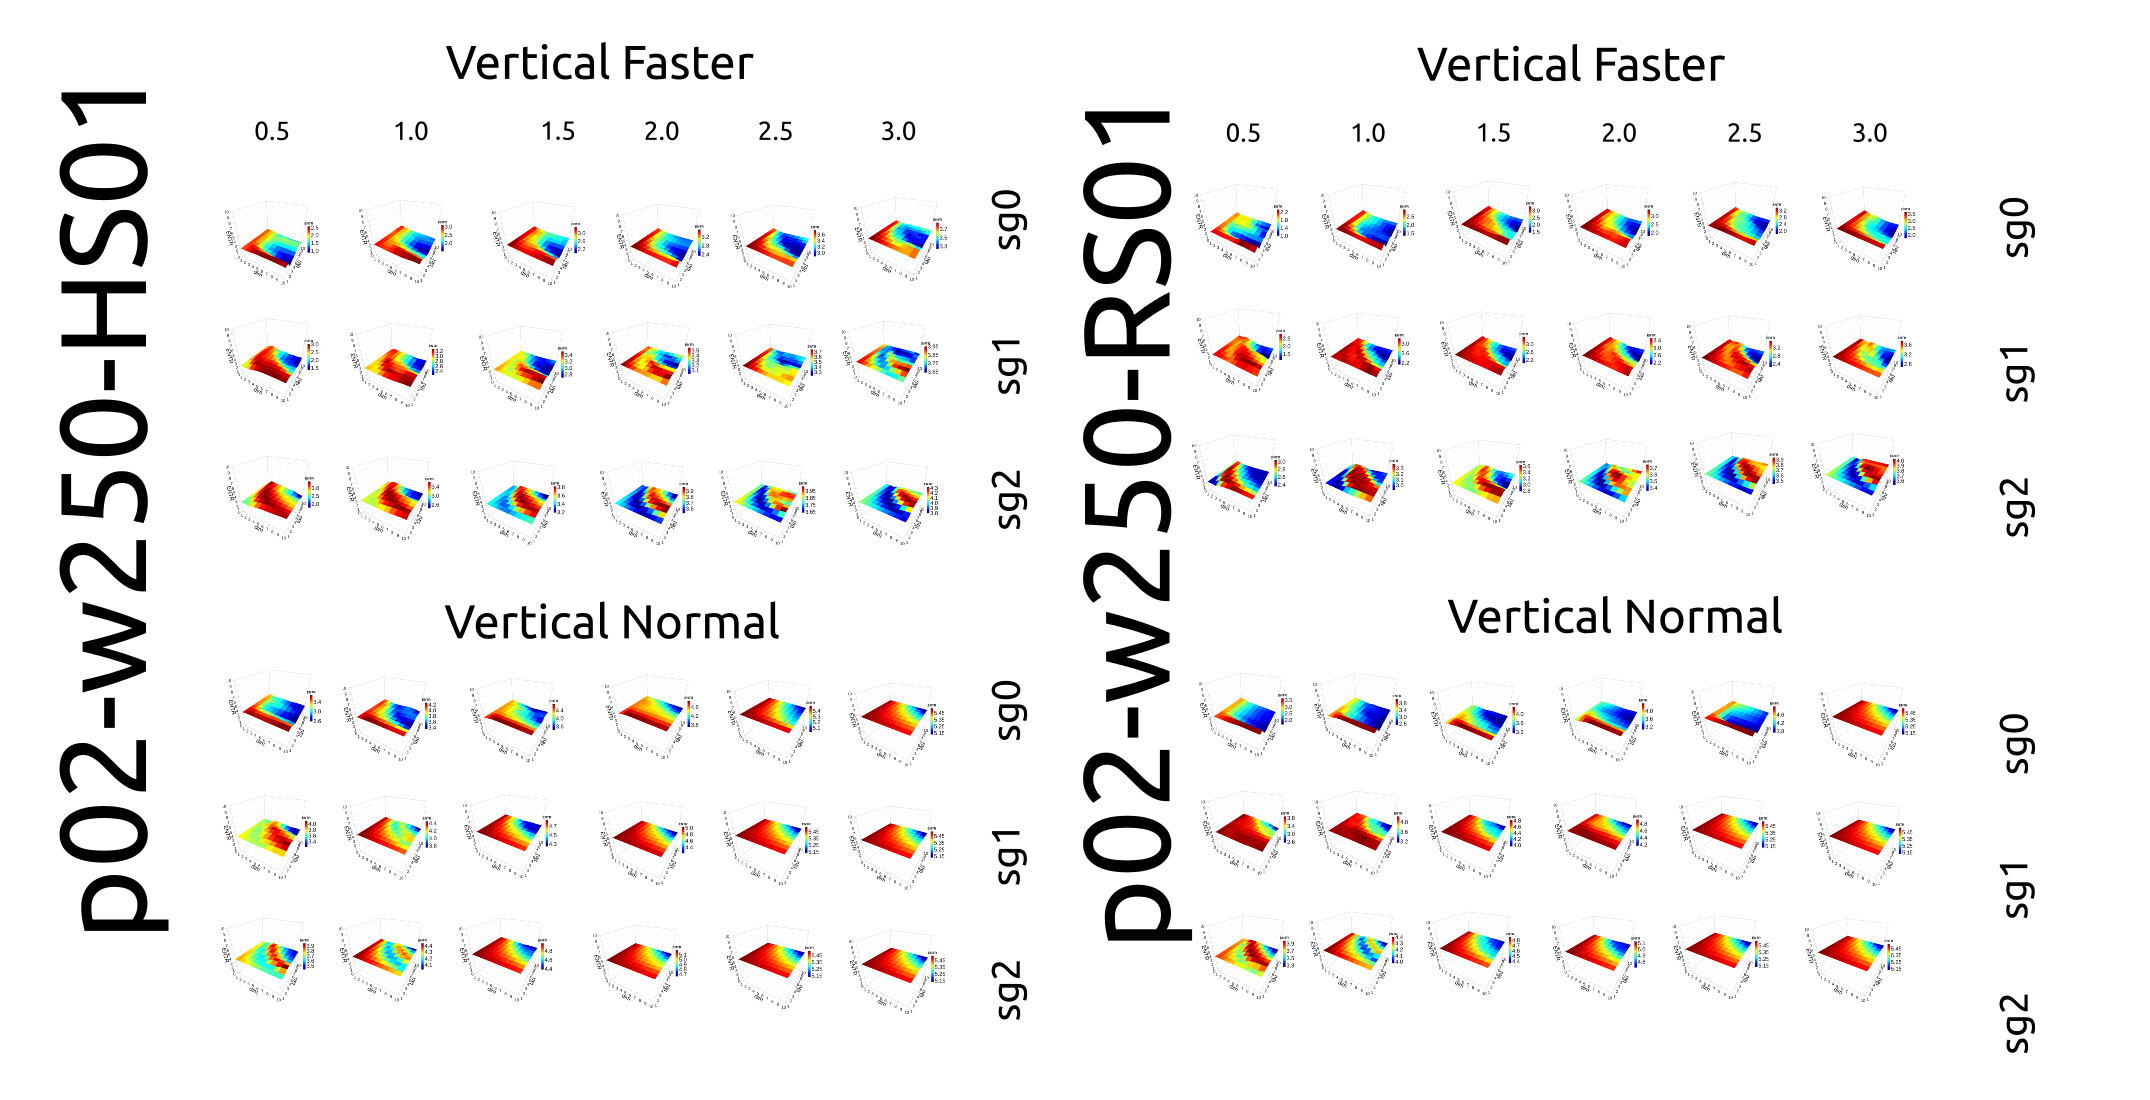
\includegraphics{figures/rqa/output/epsilons/rqa-epsilonsp02w250Vertical}
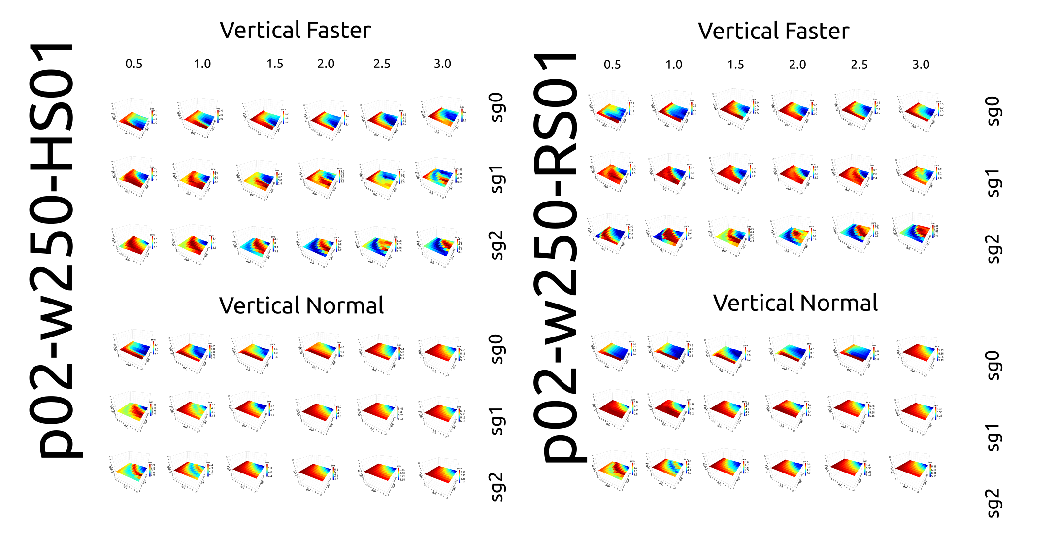
\includegraphics{sm-fig12}
    	\caption{
	{\bf RQA-Entr for participant 02 performing vertical movements for a window size of 250 samples.}
		%RQA-Entr surface plots are for participant $p02$
		%for horizontal and vertical arm movements in normal
		%and faster velocity (HN, HF, VN, VF)
		%with the normalised GyroZ or GyroY axis
		%((sg0) raw-normalised (sg0zmuv),
		%(sg1) normalised-smoothed 1 and
		%(sg1) normalised-smoothed 2)
		%and with one sensor attached to the participant (HS01)
		%and other sensor attached to the robot (RS01).
	Code and data to reproduce the figure is available in \cite{srep2021}.
        }
    \label{fig-p02-V-w250}
\end{figure}
%---------------------------------(FIGURE)------------------------------------


\newpage
%---------------------------------FIGURE)-------------------------------------
\begin{figure}[ht!]
\centering
%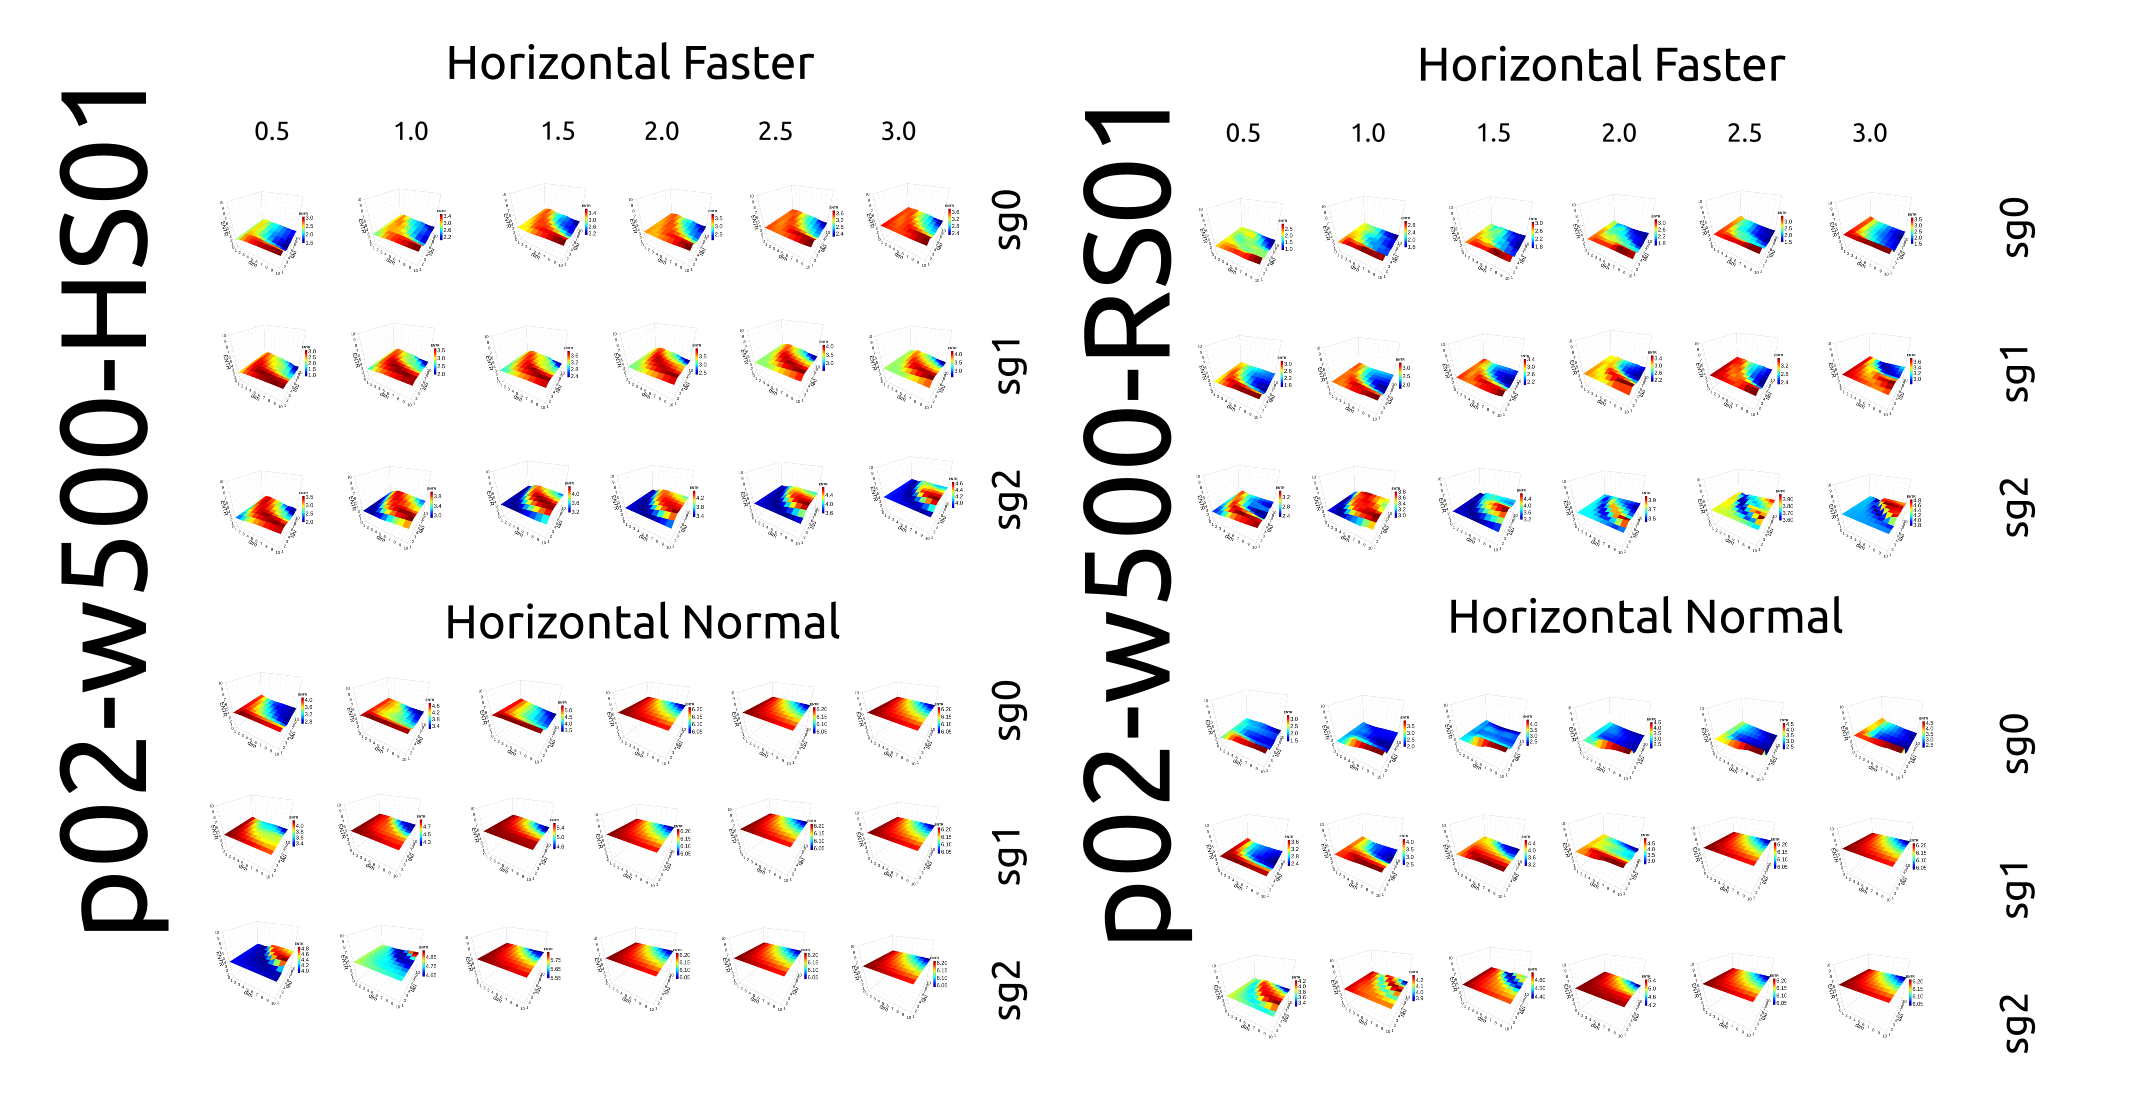
\includegraphics{figures/rqa/output/epsilons/rqa-epsilonsp02w500Horizontal}
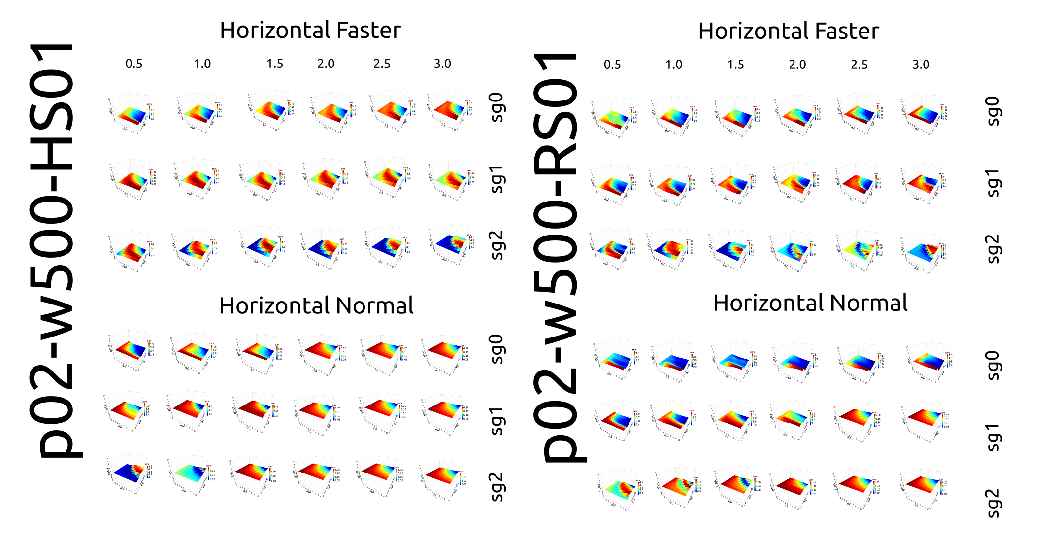
\includegraphics{sm-fig13}
    	\caption{
	{\bf RQA-Entr for participant 02 performing horizontal movements for a window size of 500 samples.}
		%RQA-Entr surface plots are for participant $p02$
		%for horizontal and vertical arm movements in normal
		%and faster velocity (HN, HF, VN, VF)
		%with the normalised GyroZ or GyroY axis
		%((sg0) raw-normalised (sg0zmuv),
		%(sg1) normalised-smoothed 1 and
		%(sg1) normalised-smoothed 2)
		%and with one sensor attached to the participant (HS01)
		%and other sensor attached to the robot (RS01).
	Code and data to reproduce the figure is available in \cite{srep2021}.
        }
    \label{fig-p02-H-w500}
\end{figure}
%---------------------------------(FIGURE)------------------------------------
%---------------------------------FIGURE)-------------------------------------
\begin{figure}[hb!]
\centering
%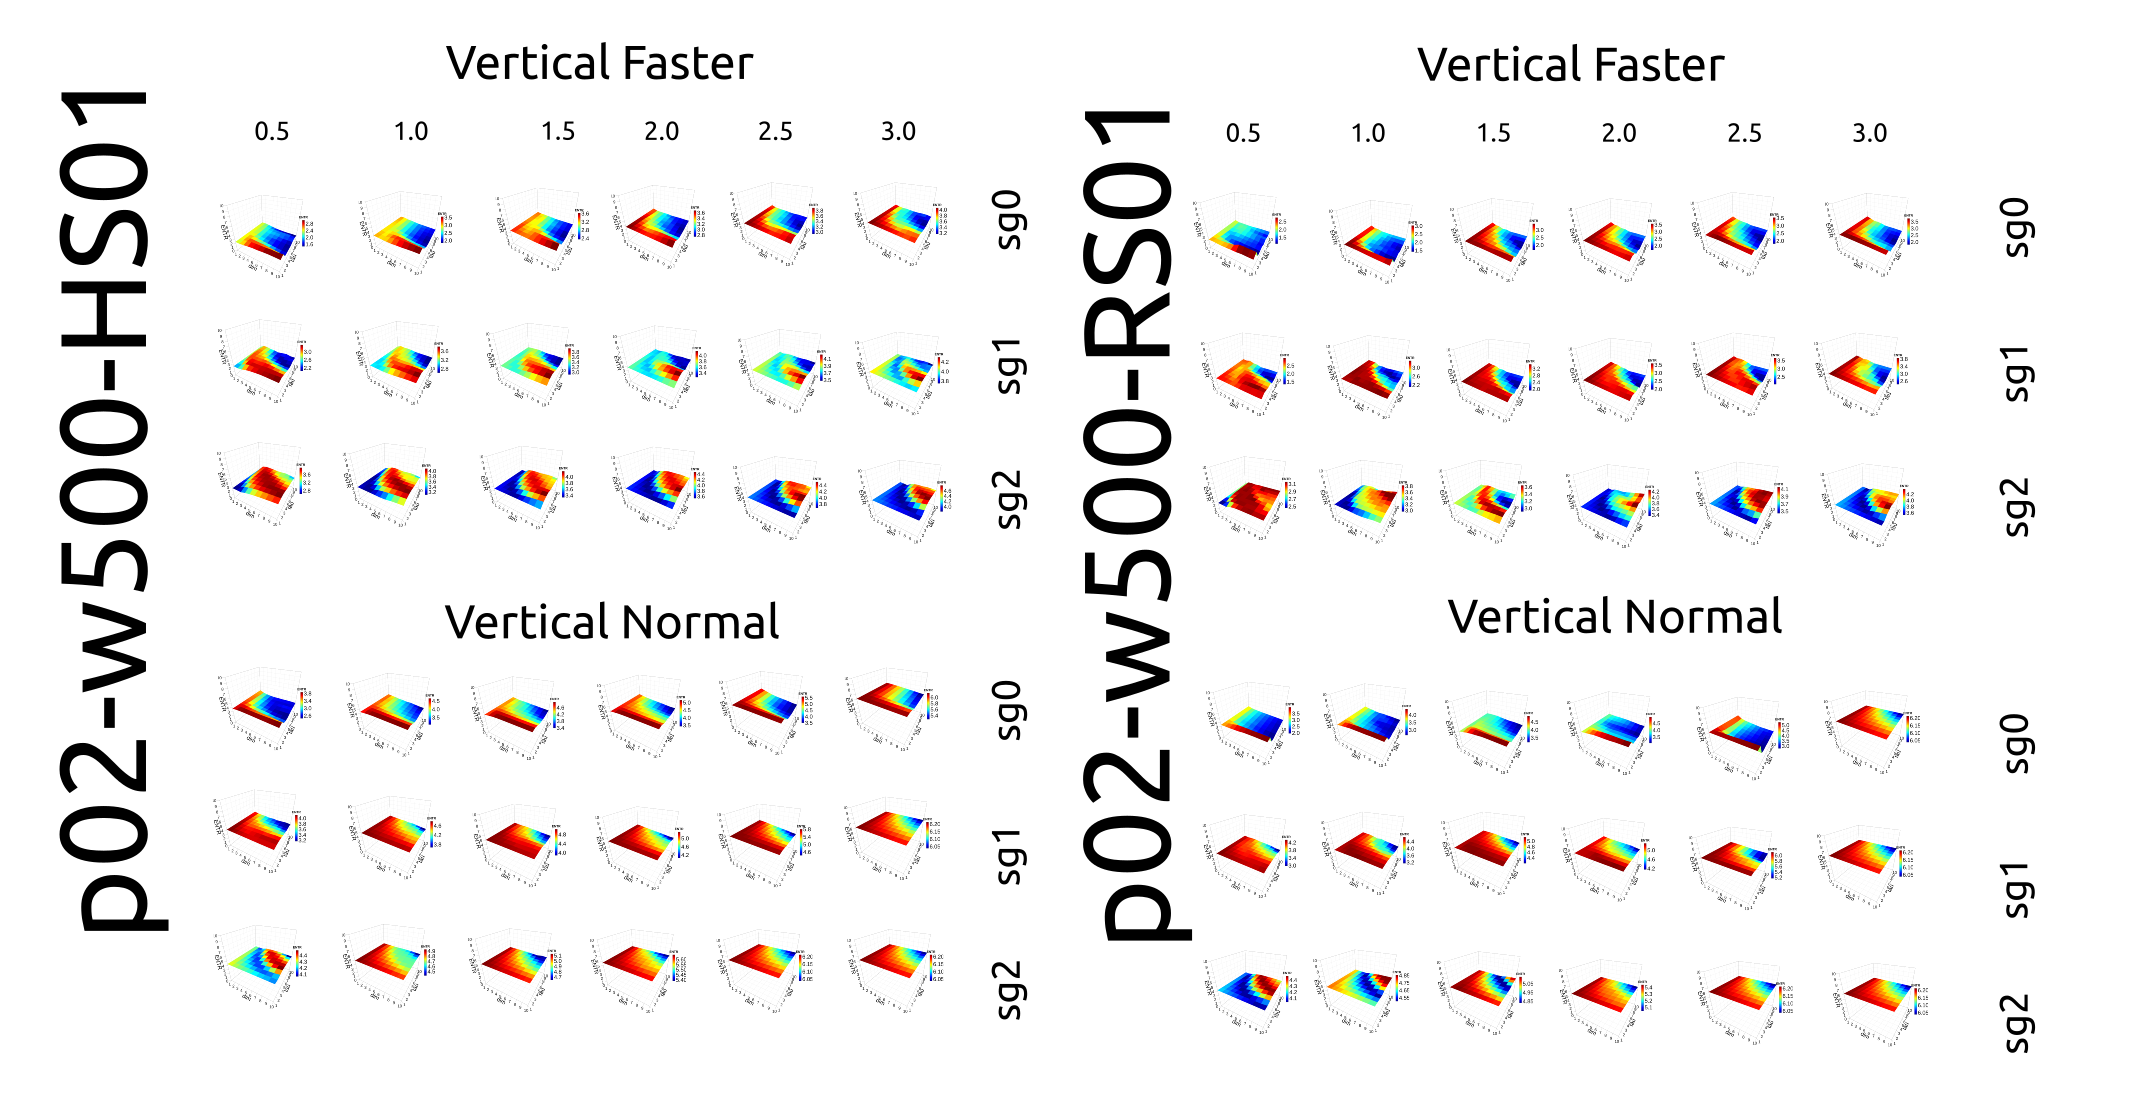
\includegraphics{figures/rqa/output/epsilons/rqa-epsilonsp02w500Vertical}
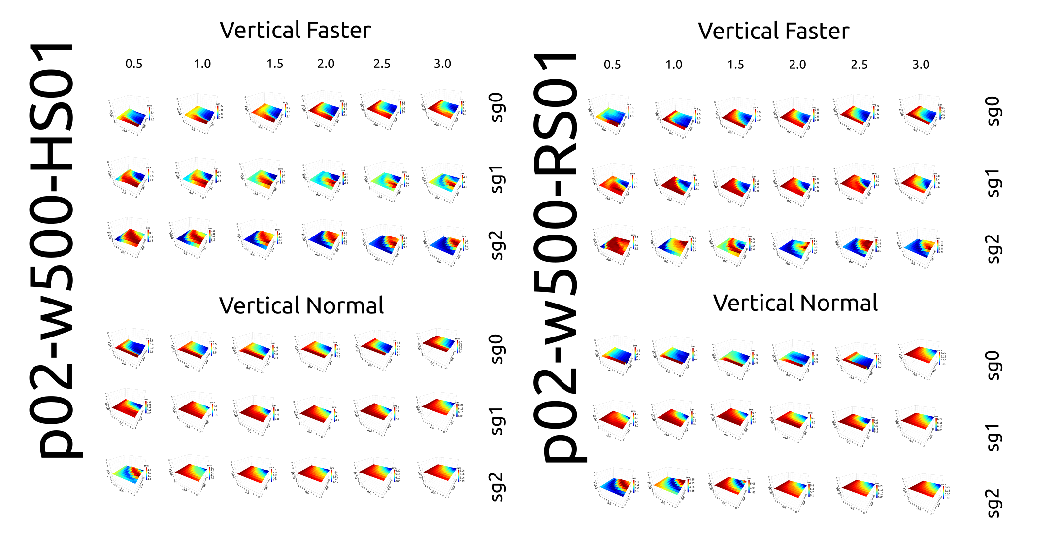
\includegraphics{sm-fig14}
    	\caption{
	{\bf RQA-Entr for participant 02 performing vertical movements for a window size of 500 samples.}
		%RQA-Entr surface plots are for participant $p02$
		%for horizontal and vertical arm movements in normal
		%and faster velocity (HN, HF, VN, VF)
		%with the normalised GyroZ or GyroY axis
		%((sg0) raw-normalised (sg0zmuv),
		%(sg1) normalised-smoothed 1 and
		%(sg1) normalised-smoothed 2)
		%and with one sensor attached to the participant (HS01)
		%and other sensor attached to the robot (RS01).
	Code and data to reproduce the figure is available in \cite{srep2021}.
        }
    \label{fig-p02-V-w500}
\end{figure}
%---------------------------------(FIGURE)------------------------------------


\newpage
%---------------------------------FIGURE)-------------------------------------
\begin{figure}[ht!]
\centering
%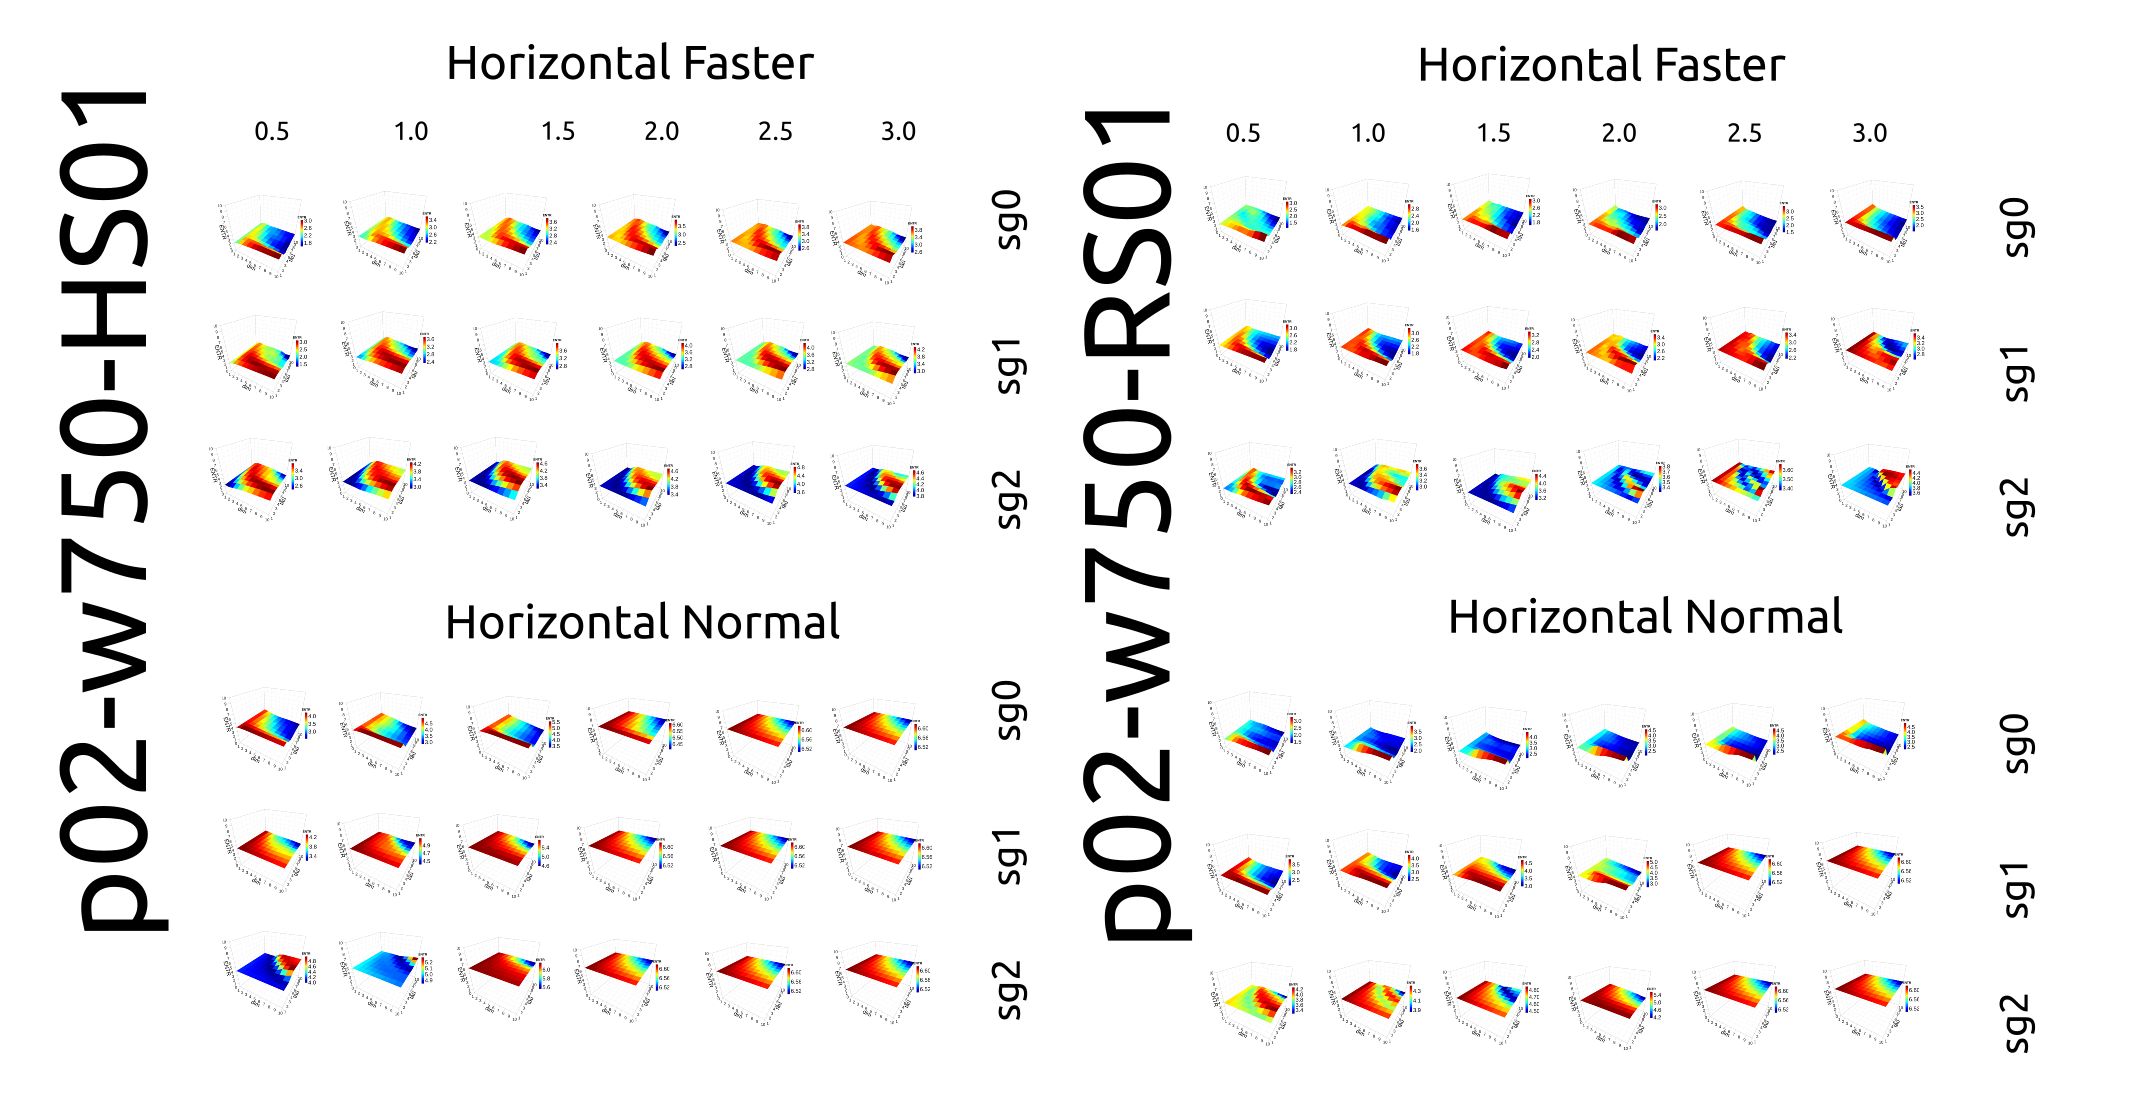
\includegraphics{figures/rqa/output/epsilons/rqa-epsilonsp02w750Horizontal}
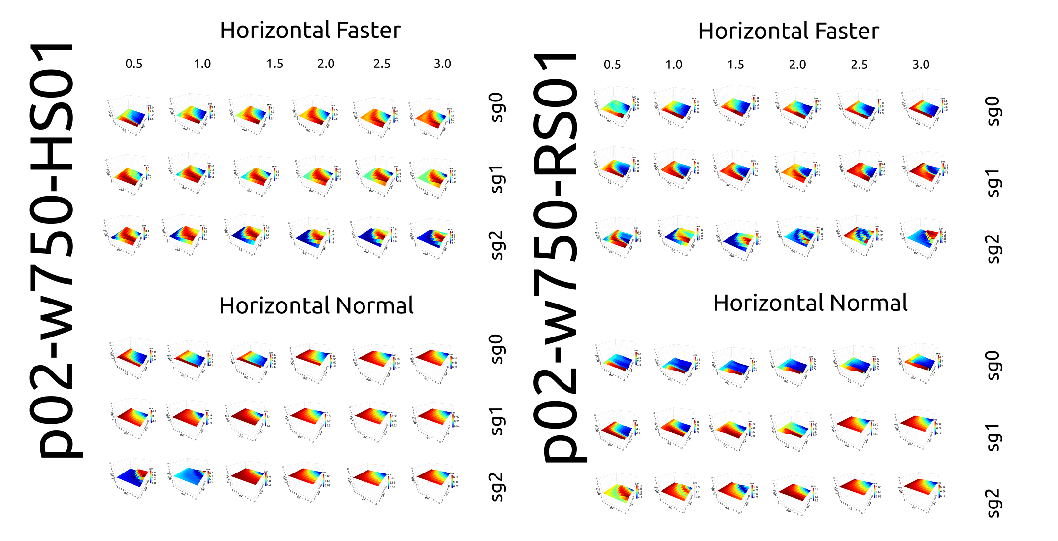
\includegraphics{sm-fig15}
    	\caption{
	{\bf RQA-Entr for participant 02 performing horizontal movements for a window size of 750 samples.}
		%RQA-Entr surface plots are for participant $p02$
		%for horizontal and vertical arm movements in normal
		%and faster velocity (HN, HF, VN, VF)
		%with the normalised GyroZ or GyroY axis
		%((sg0) raw-normalised (sg0zmuv),
		%(sg1) normalised-smoothed 1 and
		%(sg1) normalised-smoothed 2)
		%and with one sensor attached to the participant (HS01)
		%and other sensor attached to the robot (RS01).
	Code and data to reproduce the figure is available in \cite{srep2021}.
        }
    \label{fig-p02-H-w750}
\end{figure}
%---------------------------------(FIGURE)------------------------------------
%---------------------------------FIGURE)-------------------------------------
\begin{figure}[hb!]
\centering
%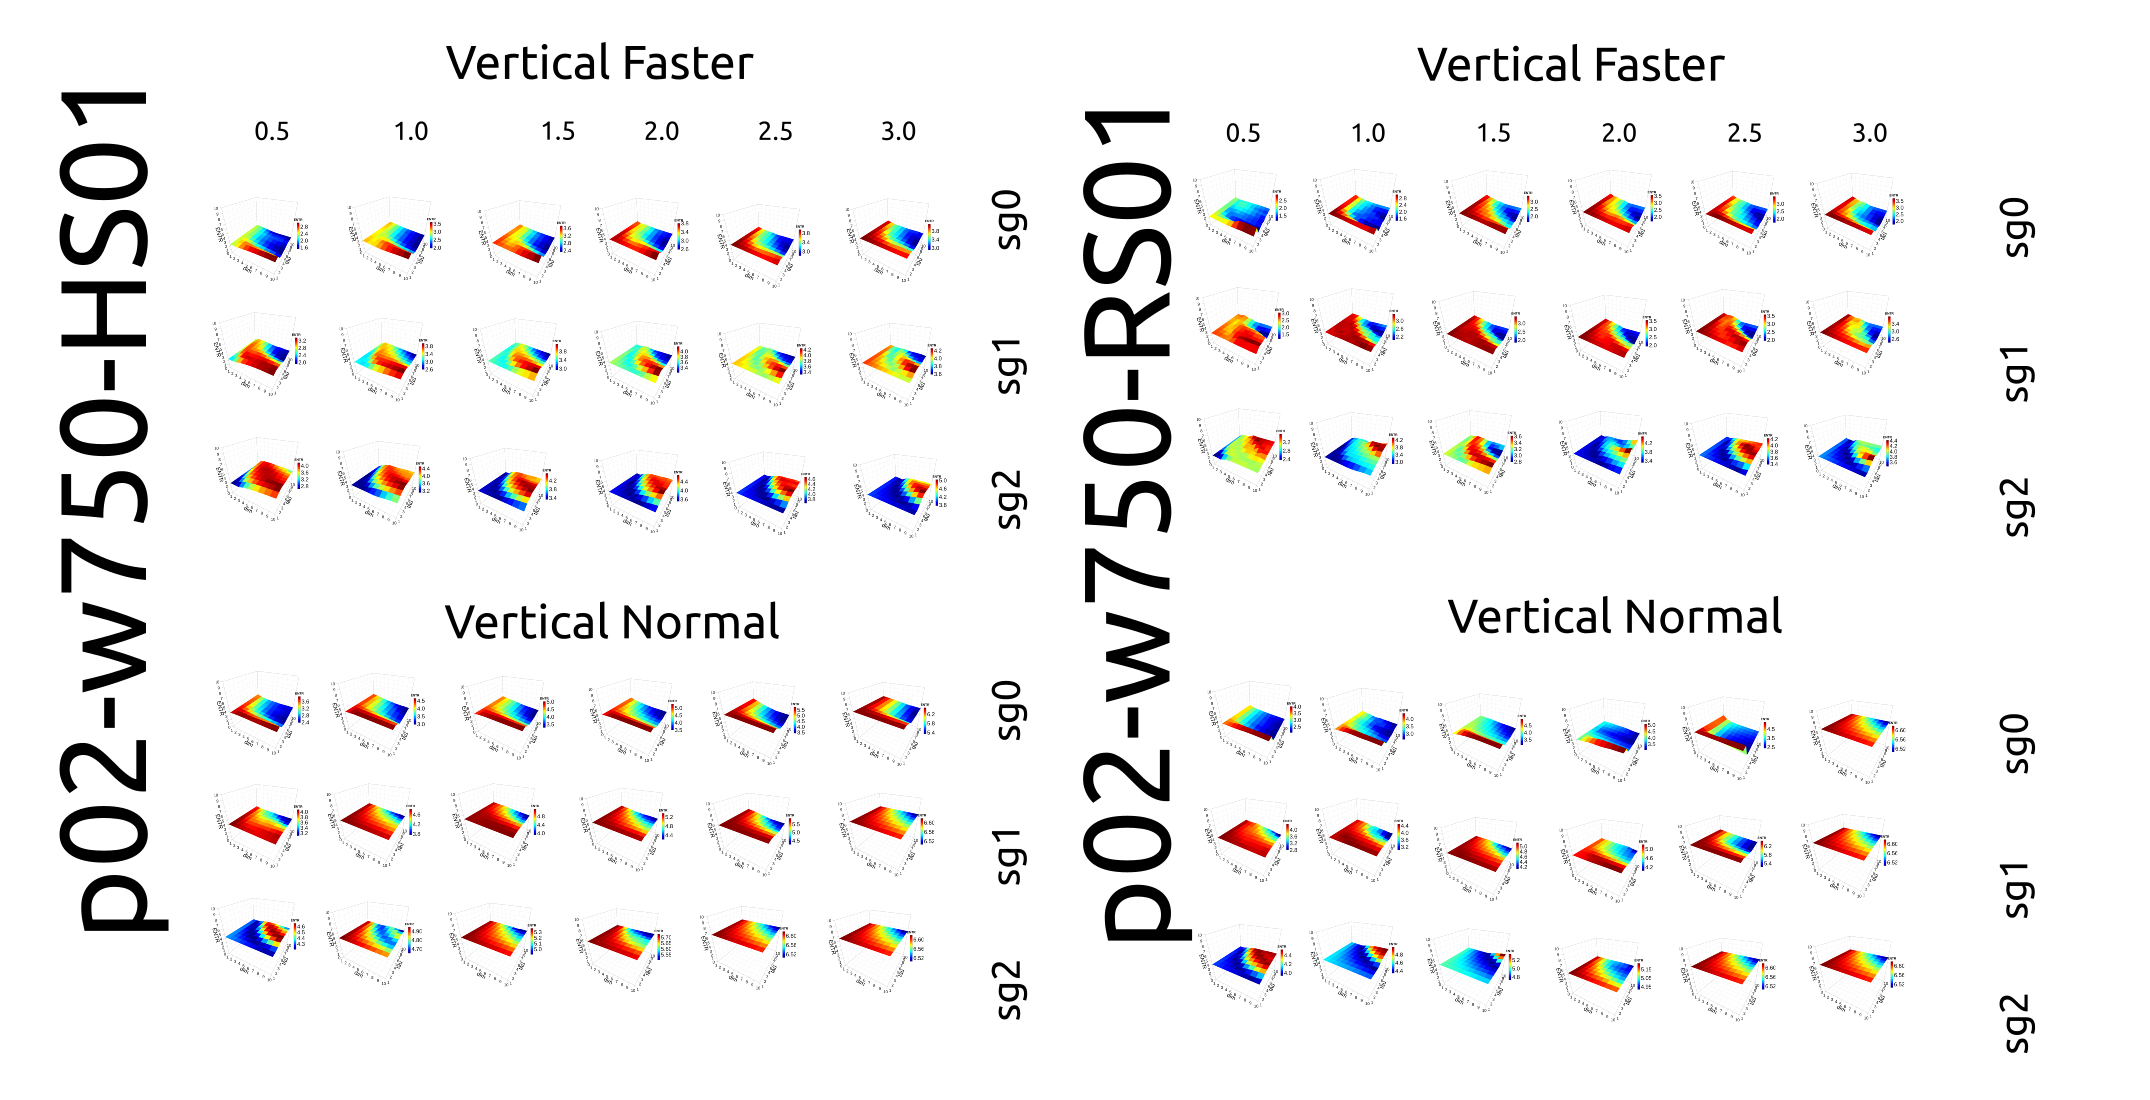
\includegraphics{figures/rqa/output/epsilons/rqa-epsilonsp02w750Vertical}
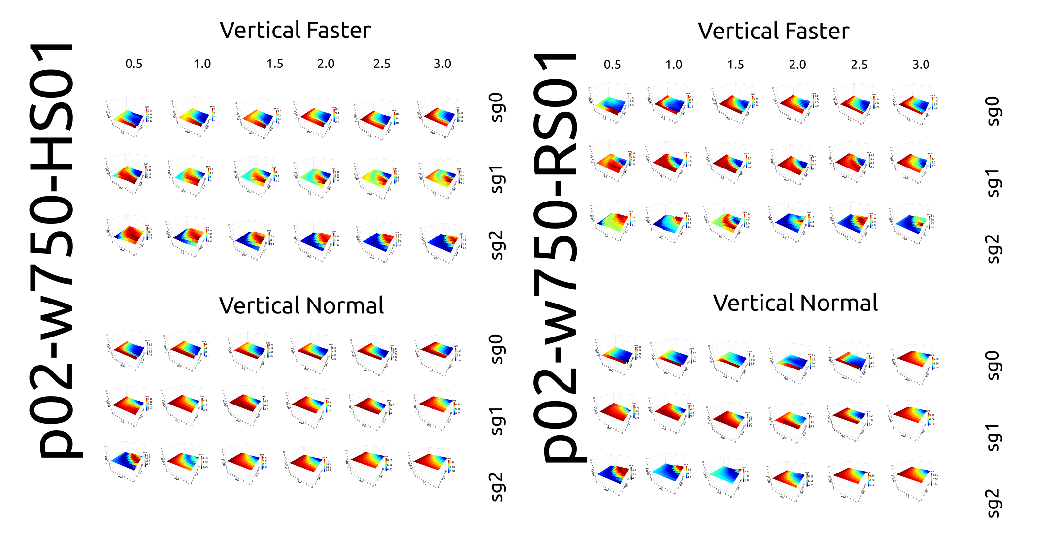
\includegraphics{sm-fig16}
    	\caption{
	{\bf RQA-Entr for participant 02 performing vertical movements for a window size of 750 samples.}
		%RQA-Entr surface plots are for participant $p02$
		%for horizontal and vertical arm movements in normal
		%and faster velocity (HN, HF, VN, VF)
		%with the normalised GyroZ or GyroY axis
		%((sg0) raw-normalised (sg0zmuv),
		%(sg1) normalised-smoothed 1 and
		%(sg1) normalised-smoothed 2)
		%and with one sensor attached to the participant (HS01)
		%and other sensor attached to the robot (RS01).
	Code and data to reproduce the figure is available in \cite{srep2021}.
        }
    \label{fig-p02-V-w750}
\end{figure}
%---------------------------------(FIGURE)------------------------------------


\newpage
\subsection{Participant 03}
%X Three level of
%X smoothness were computed for RQA metrics showing smoothed 3D surfaces and
%X the level of smoothness increase (Fig.~\ref{fig:topo_smoothness}).
%After data collection, raw time series were windowed, normalised and
%smoothed. Then, due to space limitations and to have simple visualisation,
Figures \ref{fig-p03-H-w100} and \ref{fig-p03-V-w100} are for a window size of 100 samples.
Figures \ref{fig-p03-H-w250} and \ref{fig-p03-V-w250} are for a window size of 250 samples.
Figures \ref{fig-p03-H-w500} and \ref{fig-p03-V-w500} are for a window size of 500 samples.
Figures \ref{fig-p03-H-w750} and \ref{fig-p03-V-w750} are for a window size of 750 samples.


\newpage
%---------------------------------FIGURE)-------------------------------------
\begin{figure}[ht!]
\centering
%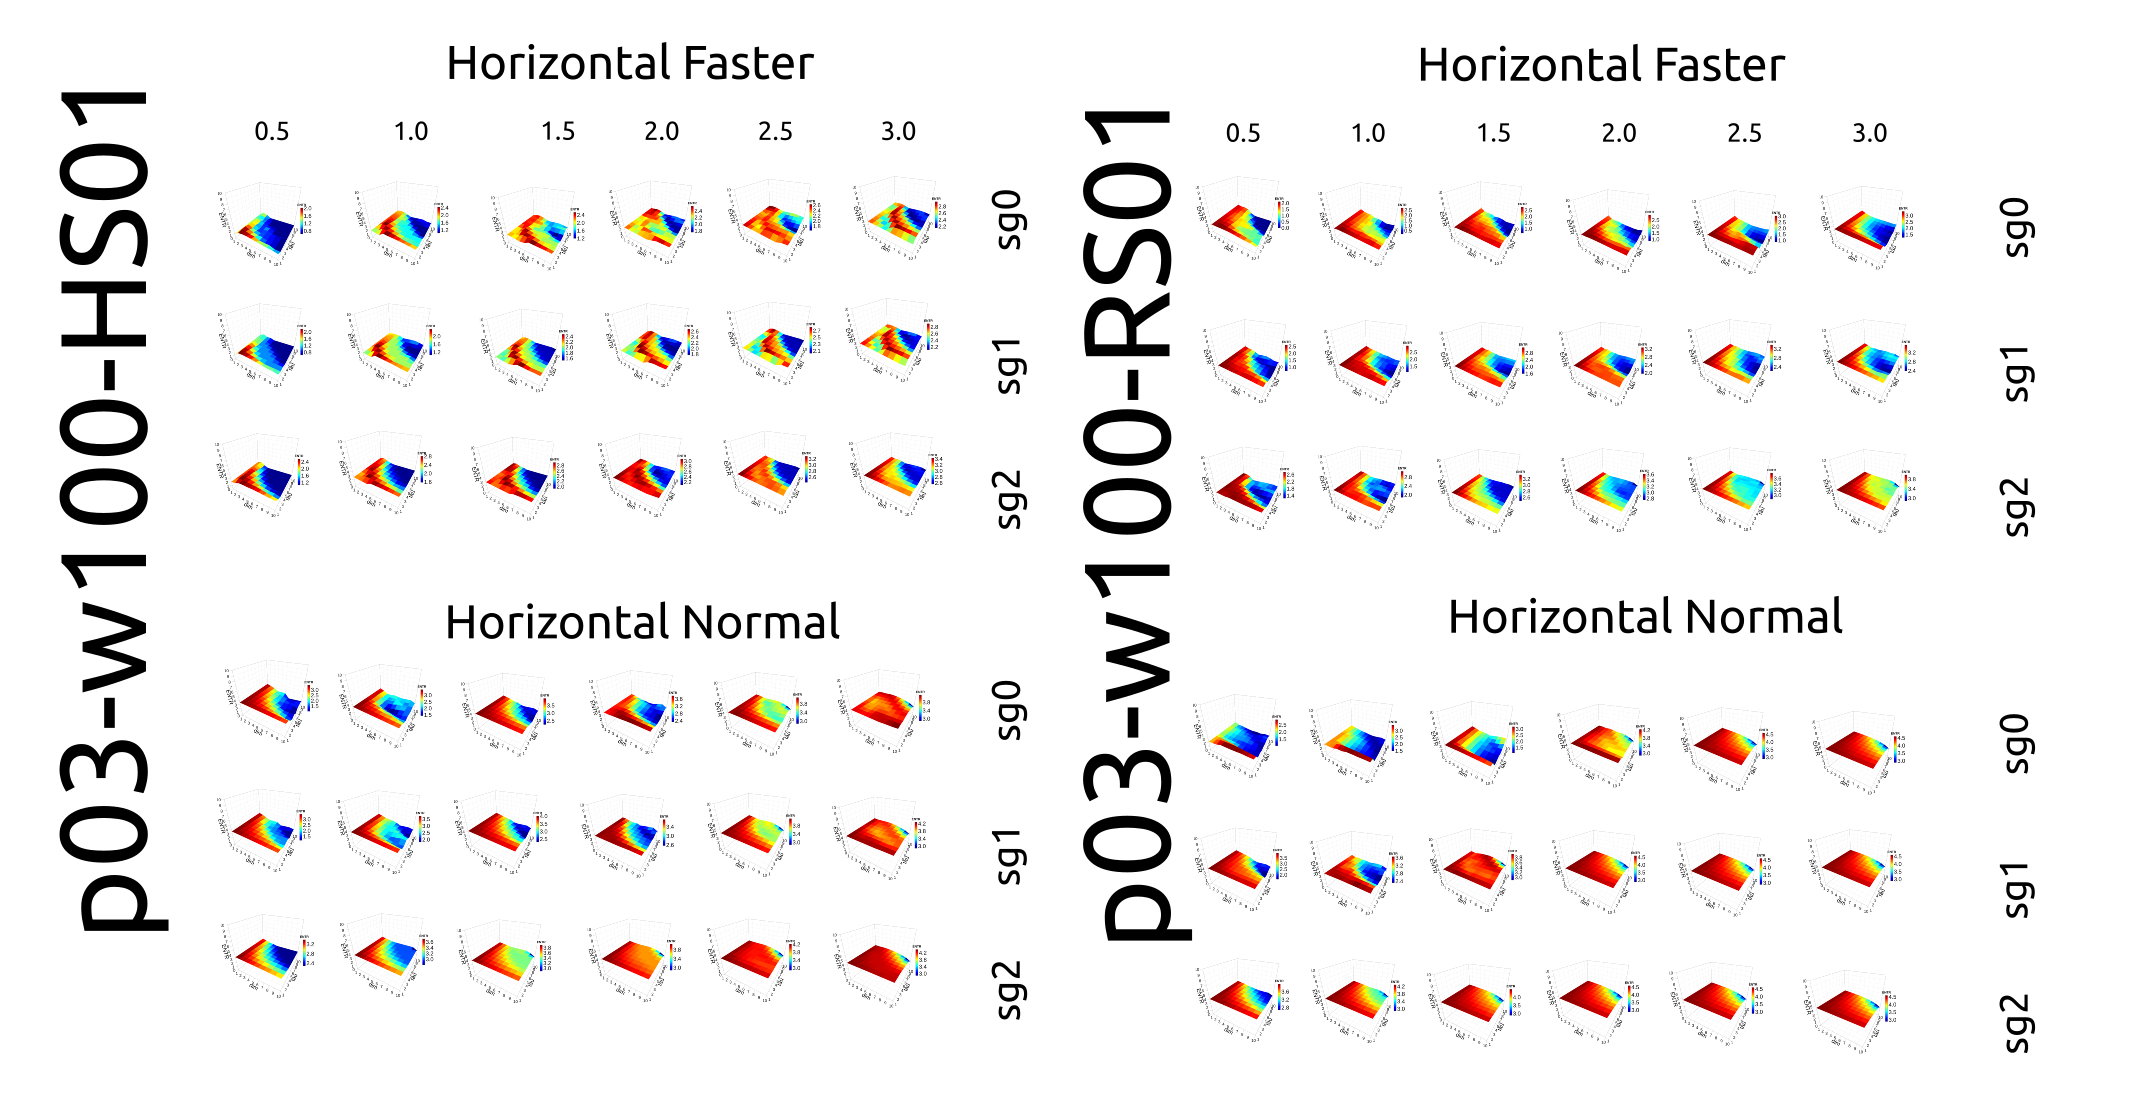
\includegraphics[scale=1.0]{figures/rqa/output/epsilons/rqa-epsilonsp03w100Horizontal}
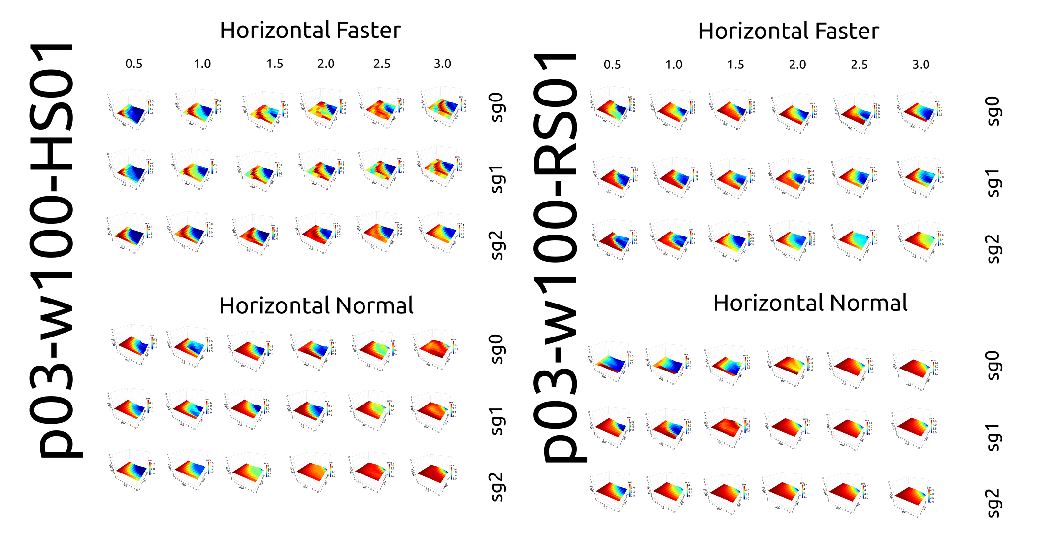
\includegraphics[scale=1.0]{sm-fig17}
    	\caption{
	{\bf RQA-Entr for participant 03 performing horizontal movements for a window size of 100 samples.}
		%RQA-Entr surface plots are for participant $p03$
		%for horizontal and vertical arm movements in normal
		%and faster velocity (HN, HF, VN, VF)
		%with the normalised GyroZ or GyroY axis
		%((sg0) raw-normalised (sg0zmuv),
		%(sg1) normalised-smoothed 1 and
		%(sg1) normalised-smoothed 2)
		%and with one sensor attached to the participant (HS01)
		%and other sensor attached to the robot (RS01).
	Code and data to reproduce the figure is available in \cite{srep2021}.
        }
    \label{fig-p03-H-w100}
\end{figure}
%---------------------------------(FIGURE)------------------------------------
%---------------------------------FIGURE)-------------------------------------
\begin{figure}[hb!]
\centering
%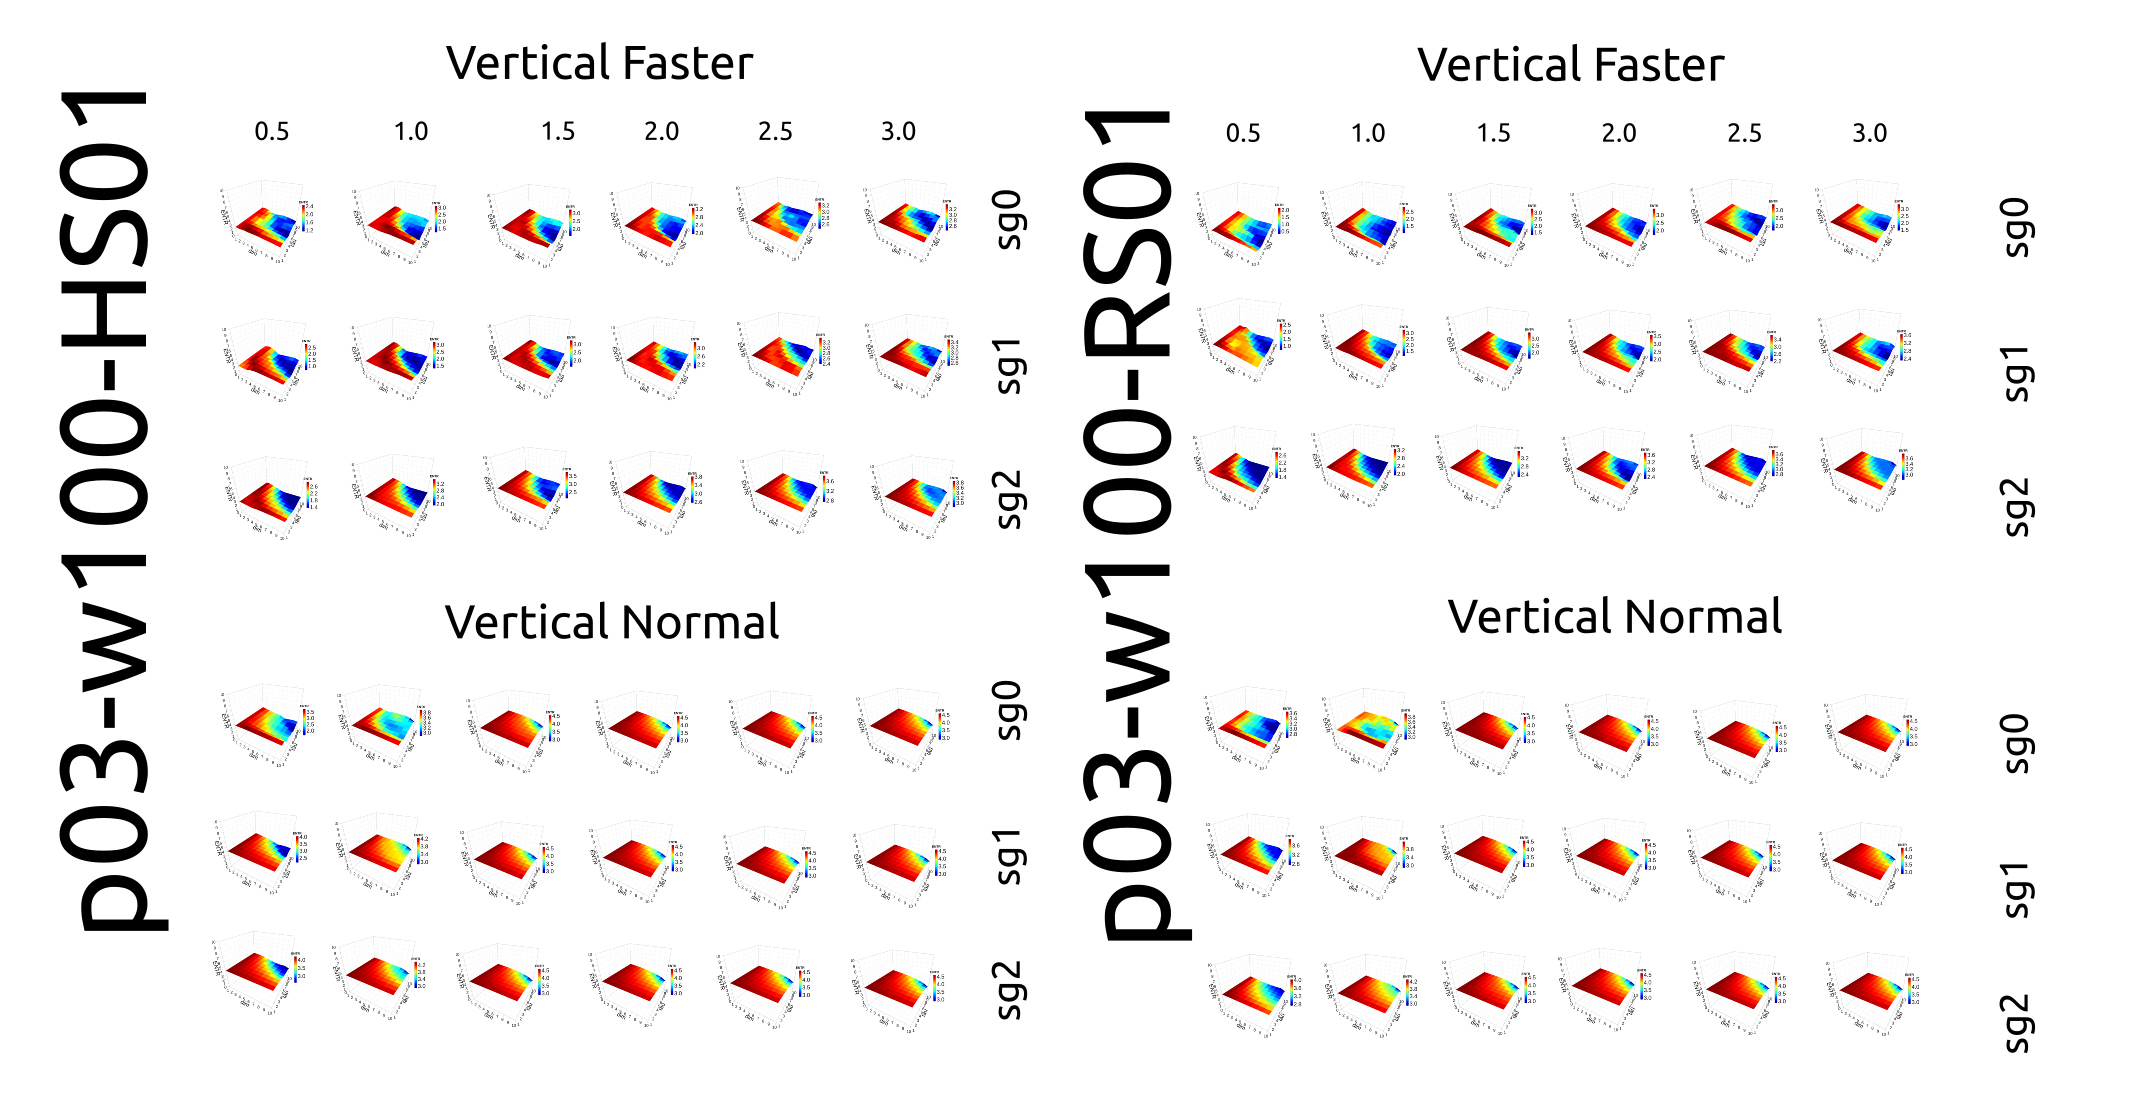
\includegraphics[scale=1.0]{figures/rqa/output/epsilons/rqa-epsilonsp03w100Vertical}
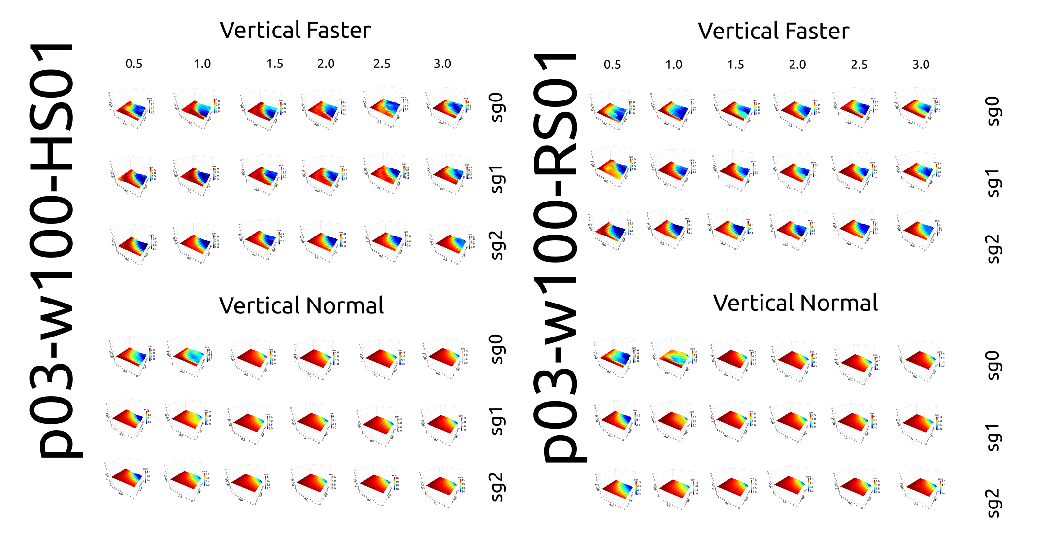
\includegraphics[scale=1.0]{sm-fig18}
    	\caption{
	{\bf RQA-Entr for participant 03 performing vertical movements for a window size of 100 samples.}
		%RQA-Entr surface plots are for participant $p03$
		%for horizontal and vertical arm movements in normal
		%and faster velocity (HN, HF, VN, VF)
		%with the normalised GyroZ or GyroY axis
		%((sg0) raw-normalised (sg0zmuv),
		%(sg1) normalised-smoothed 1 and
		%(sg1) normalised-smoothed 2)
		%and with one sensor attached to the participant (HS01)
		%and other sensor attached to the robot (RS01).
	Code and data to reproduce the figure is available in \cite{srep2021}.
        }
    \label{fig-p03-V-w100}
\end{figure}
%---------------------------------(FIGURE)------------------------------------


\newpage
%---------------------------------FIGURE)-------------------------------------
\begin{figure}[ht!]
\centering
%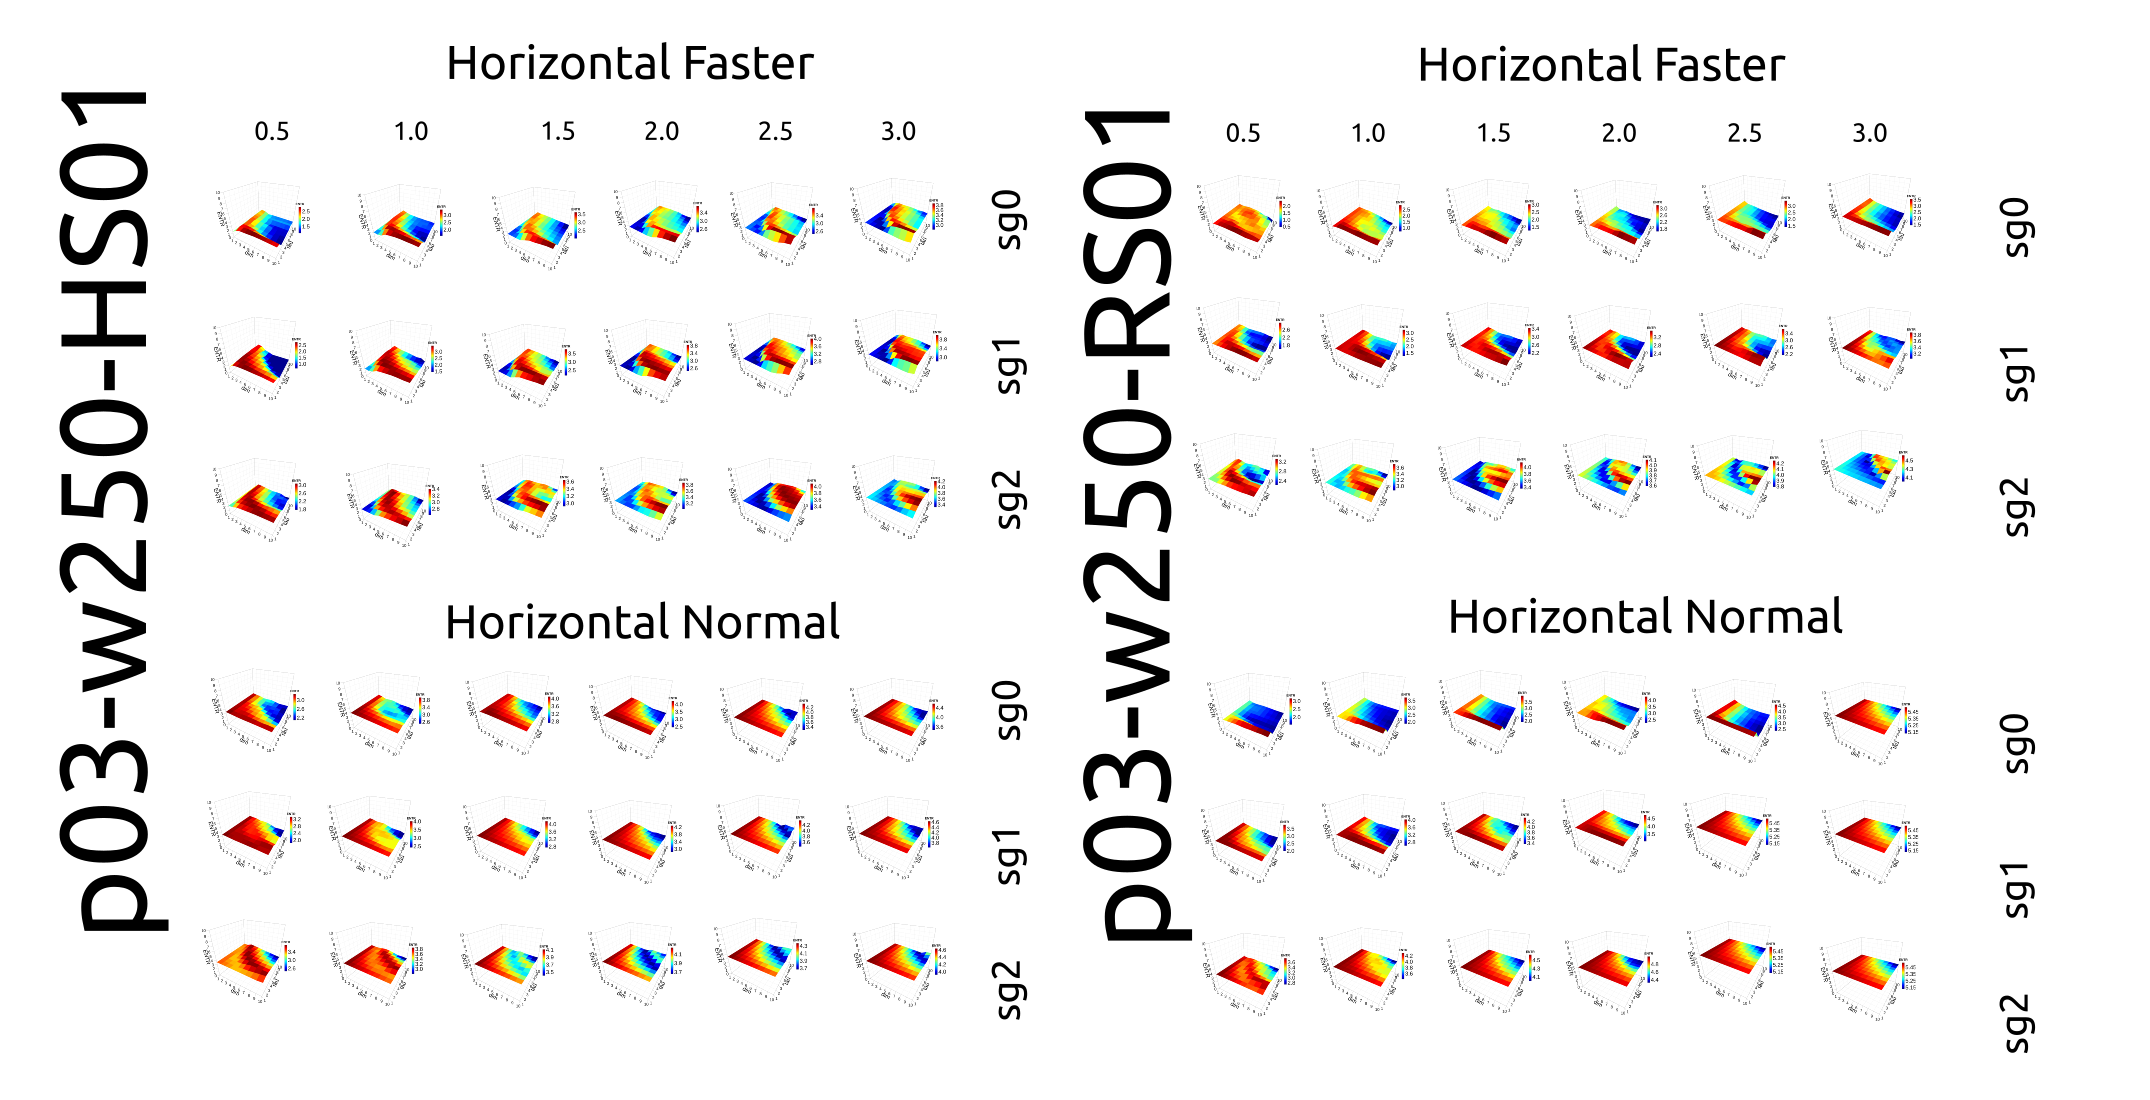
\includegraphics{figures/rqa/output/epsilons/rqa-epsilonsp03w250Horizontal}
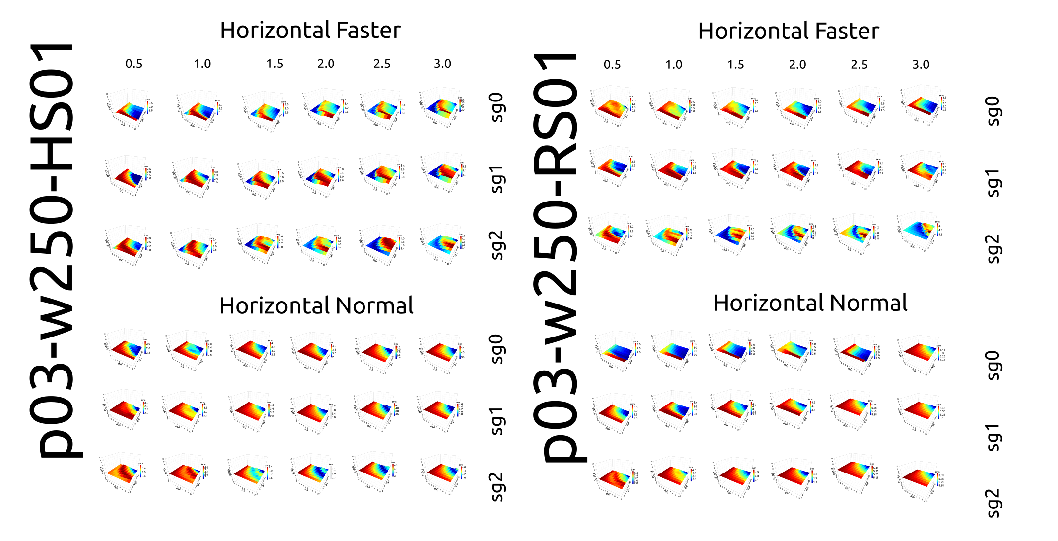
\includegraphics{sm-fig19}
    	\caption{
	{\bf RQA-Entr for participant 03 performing horizontal movements for a window size of 250 samples.}
		%RQA-Entr surface plots are for participant $p03$
		%for horizontal and vertical arm movements in normal
		%and faster velocity (HN, HF, VN, VF)
		%with the normalised GyroZ or GyroY axis
		%((sg0) raw-normalised (sg0zmuv),
		%(sg1) normalised-smoothed 1 and
		%(sg1) normalised-smoothed 2)
		%and with one sensor attached to the participant (HS01)
		%and other sensor attached to the robot (RS01).
	Code and data to reproduce the figure is available in \cite{srep2021}.
        }
    \label{fig-p03-H-w250}
\end{figure}
%---------------------------------(FIGURE)------------------------------------
%---------------------------------FIGURE)-------------------------------------
\begin{figure}[hb!]
\centering
%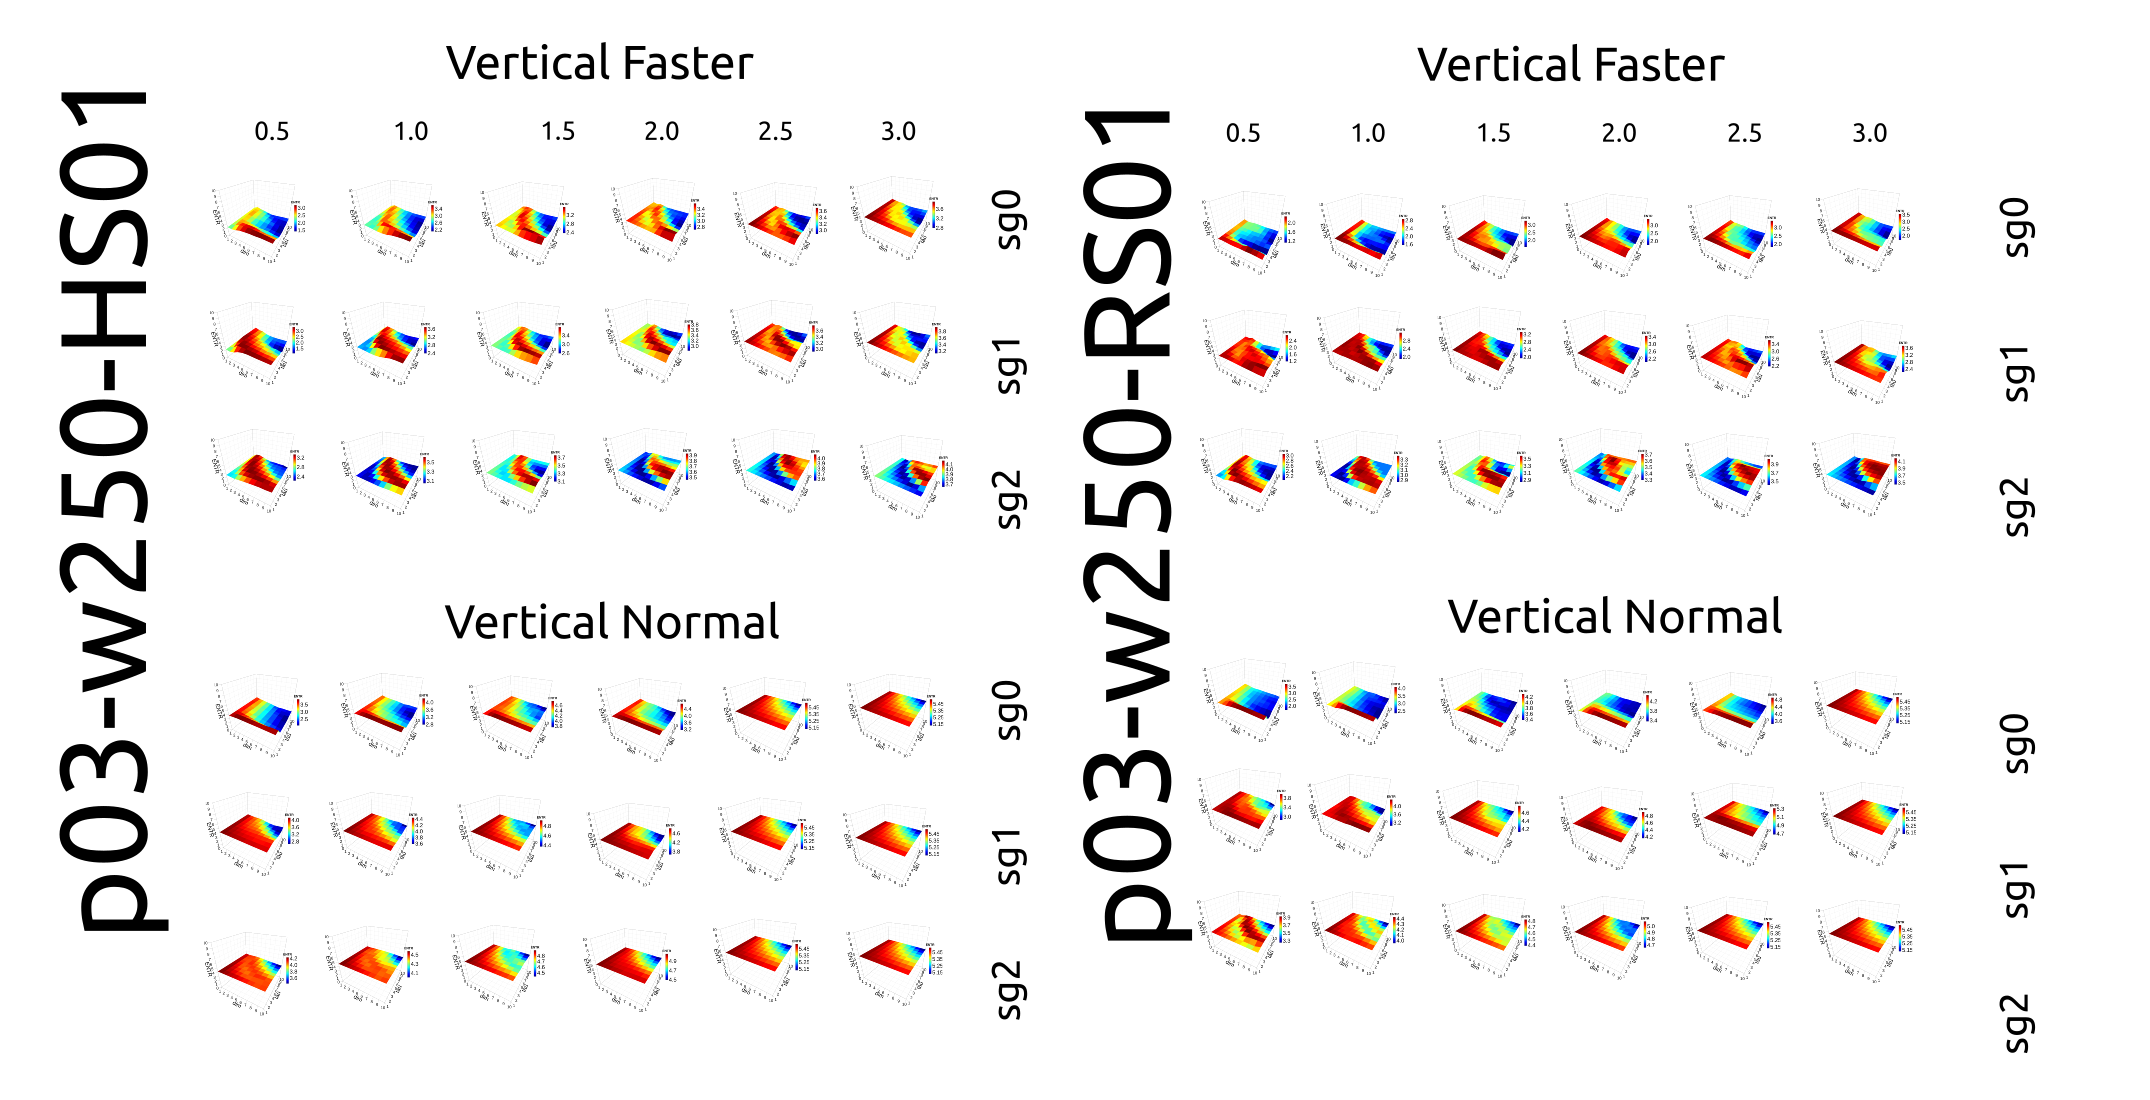
\includegraphics{figures/rqa/output/epsilons/rqa-epsilonsp03w250Vertical}
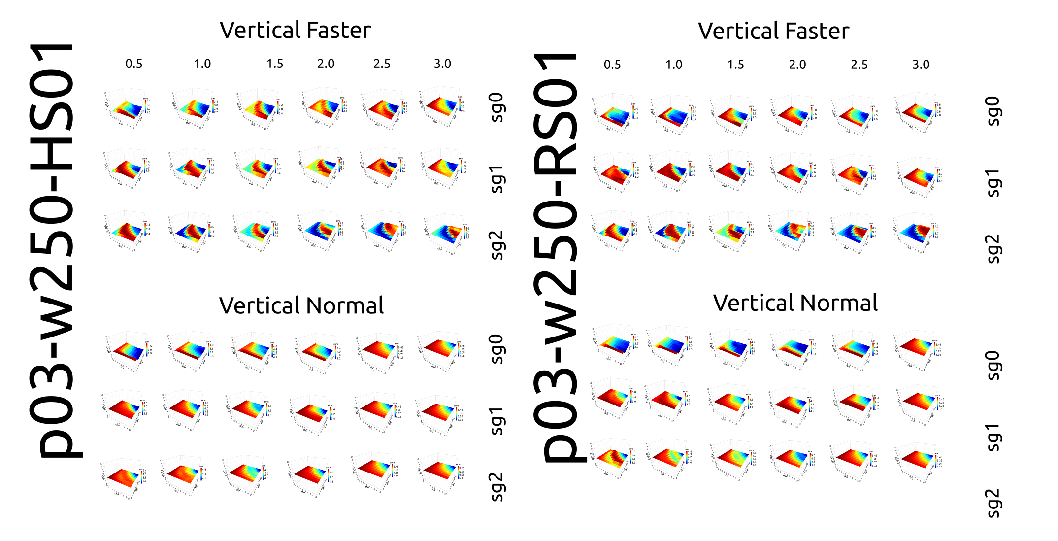
\includegraphics{sm-fig20}
    	\caption{
	{\bf RQA-Entr for participant 03 performing vertical movements for a window size of 250 samples.}
		%RQA-Entr surface plots are for participant $p03$
		%for horizontal and vertical arm movements in normal
		%and faster velocity (HN, HF, VN, VF)
		%with the normalised GyroZ or GyroY axis
		%((sg0) raw-normalised (sg0zmuv),
		%(sg1) normalised-smoothed 1 and
		%(sg1) normalised-smoothed 2)
		%and with one sensor attached to the participant (HS01)
		%and other sensor attached to the robot (RS01).
	Code and data to reproduce the figure is available in \cite{srep2021}.
        }
    \label{fig-p03-V-w250}
\end{figure}
%---------------------------------(FIGURE)------------------------------------


\newpage
%---------------------------------FIGURE)-------------------------------------
\begin{figure}[ht!]
\centering
%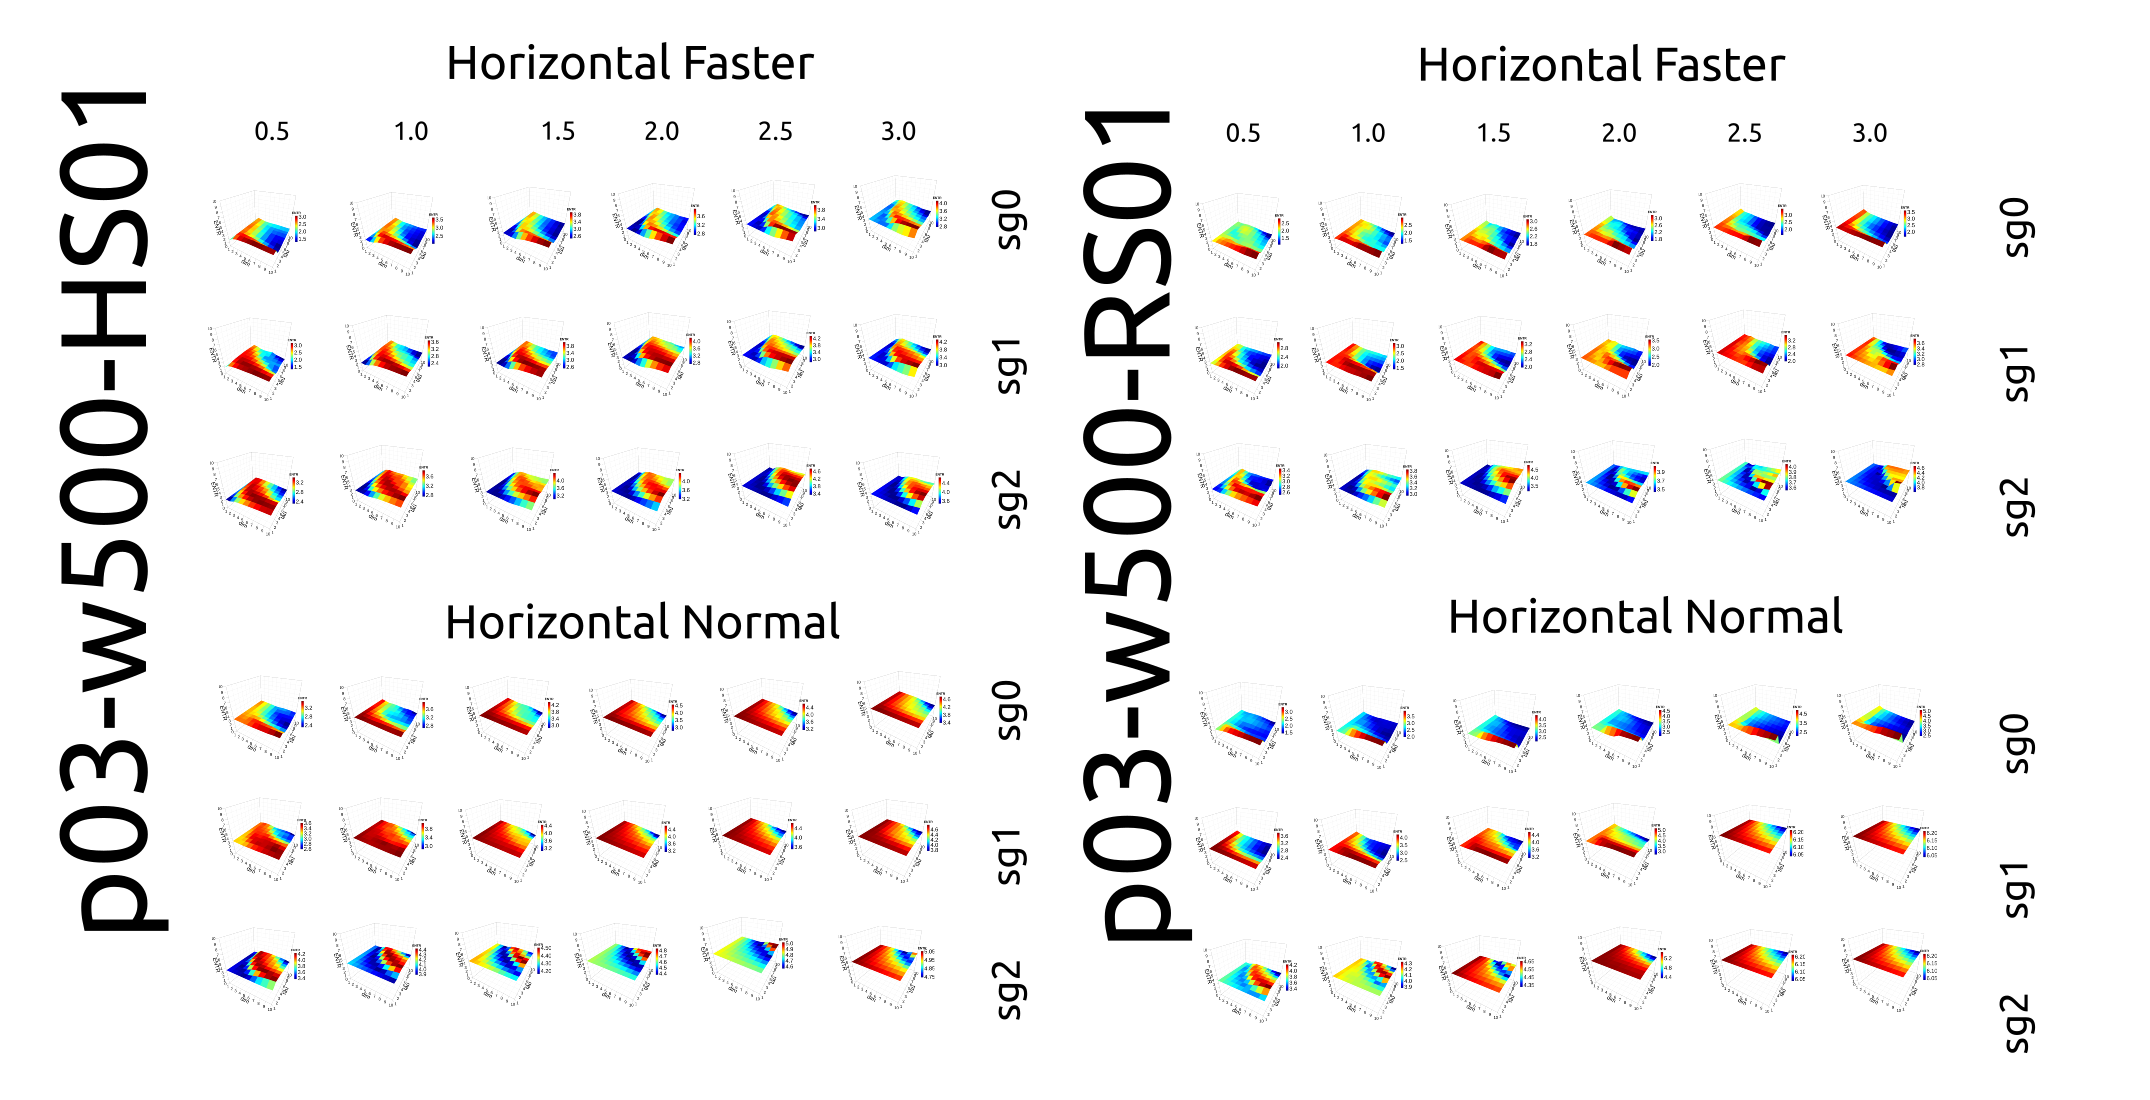
\includegraphics{figures/rqa/output/epsilons/rqa-epsilonsp03w500Horizontal}
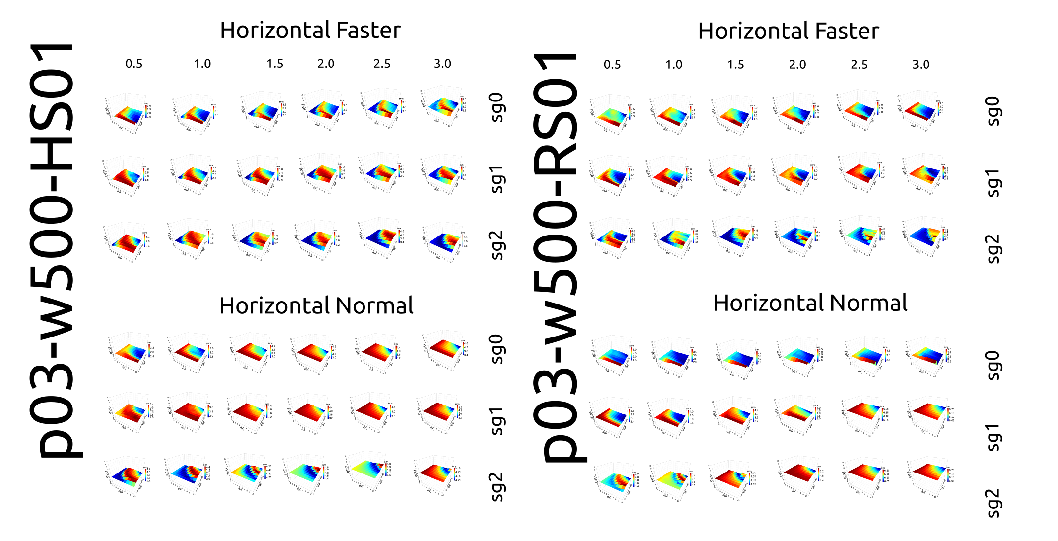
\includegraphics{sm-fig21}
    	\caption{
	{\bf RQA-Entr for participant 03 performing horizontal movements for a window size of 500 samples.}
		%RQA-Entr surface plots are for participant $p03$
		%for horizontal and vertical arm movements in normal
		%and faster velocity (HN, HF, VN, VF)
		%with the normalised GyroZ or GyroY axis
		%((sg0) raw-normalised (sg0zmuv),
		%(sg1) normalised-smoothed 1 and
		%(sg1) normalised-smoothed 2)
		%and with one sensor attached to the participant (HS01)
		%and other sensor attached to the robot (RS01).
	Code and data to reproduce the figure is available in \cite{srep2021}.
        }
    \label{fig-p03-H-w500}
\end{figure}
%---------------------------------(FIGURE)------------------------------------
%---------------------------------FIGURE)-------------------------------------
\begin{figure}[hb!]
\centering
%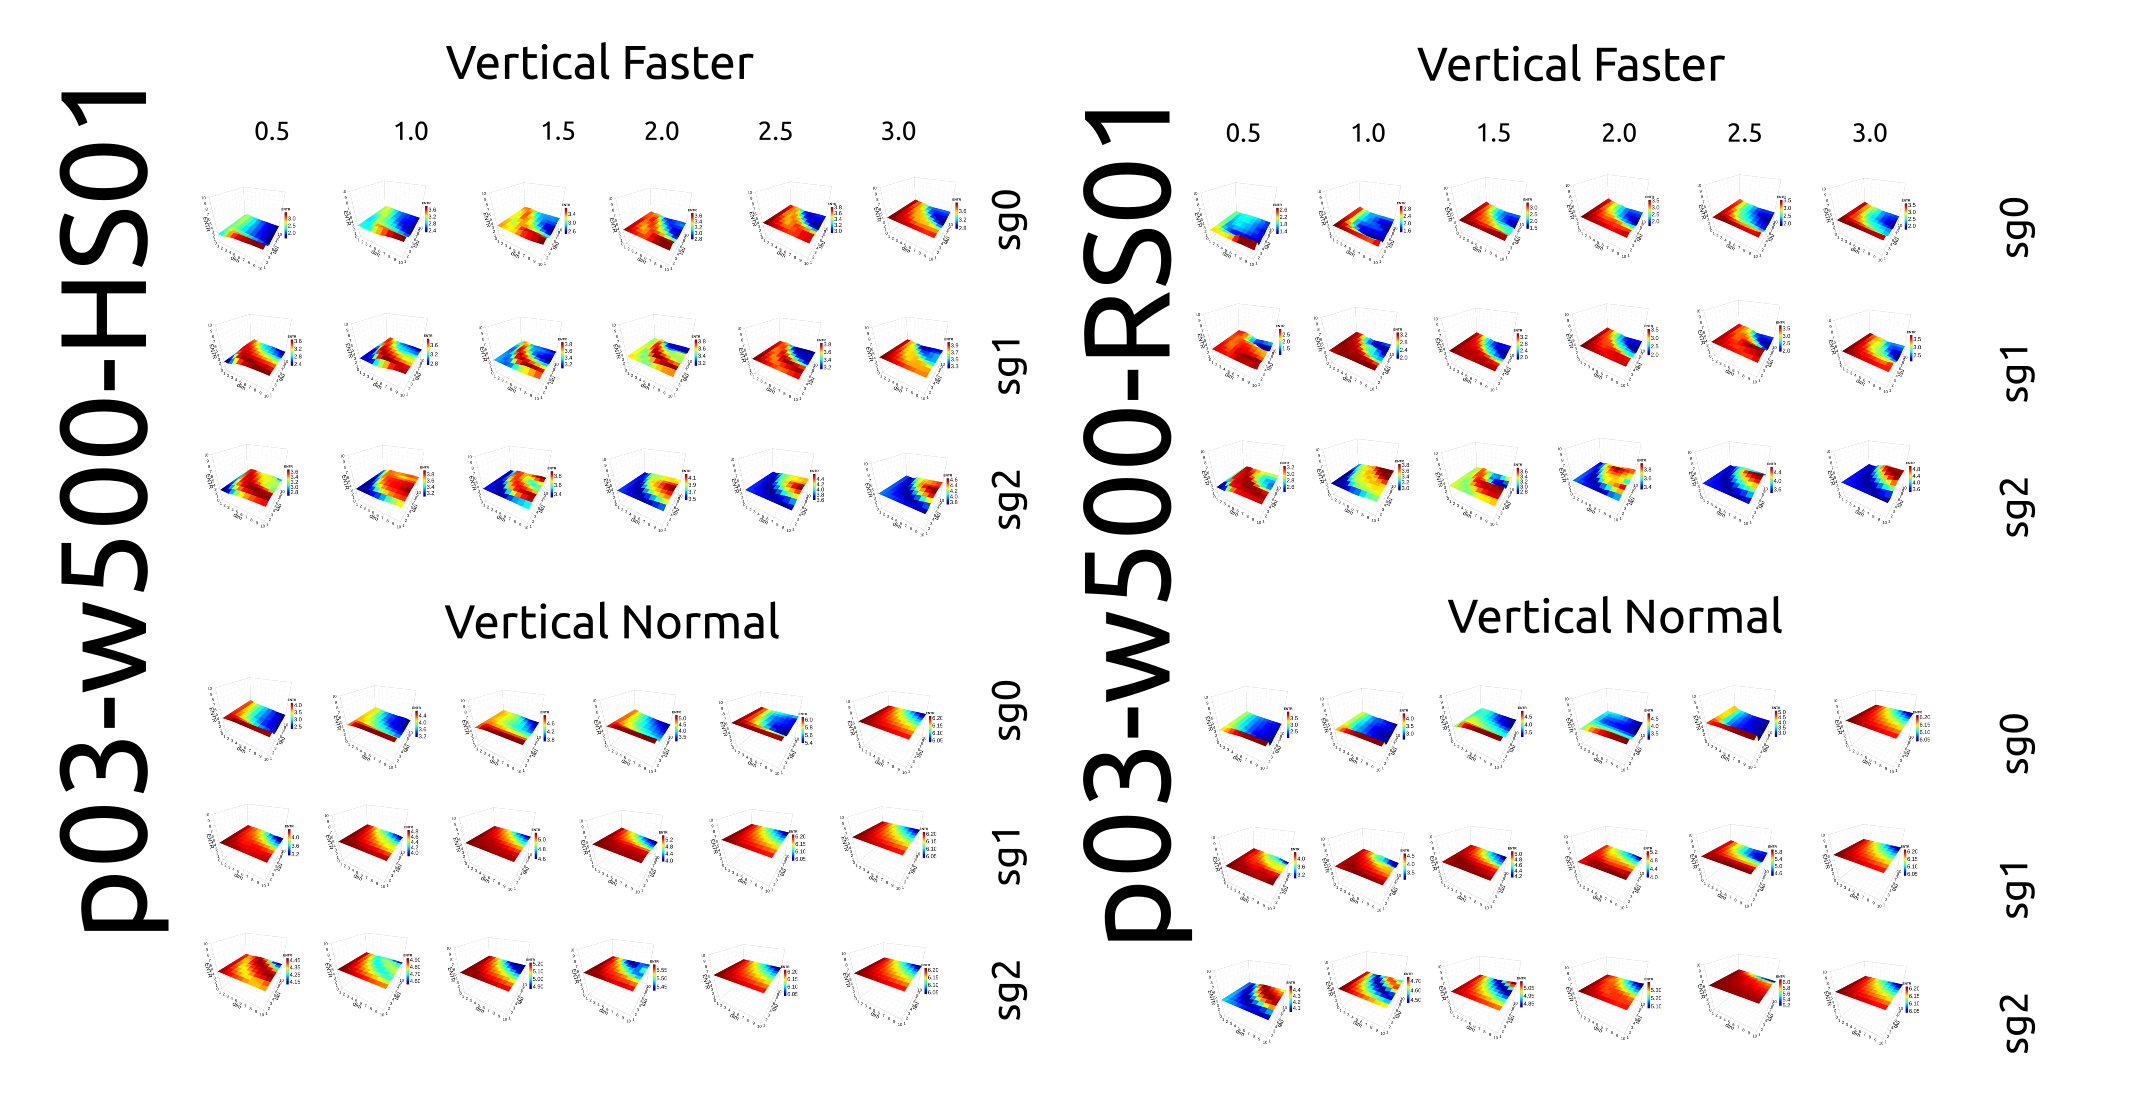
\includegraphics{figures/rqa/output/epsilons/rqa-epsilonsp03w500Vertical}
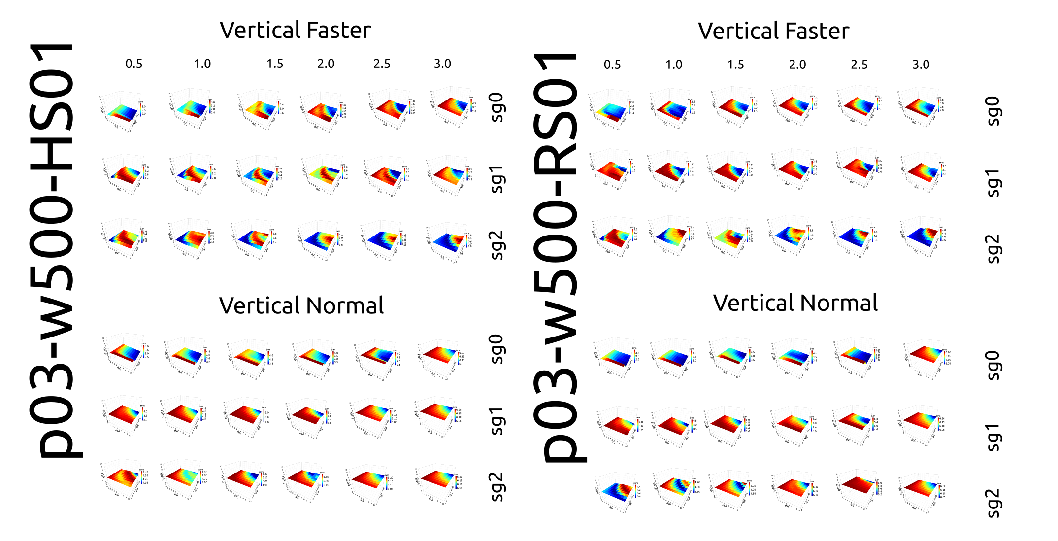
\includegraphics{sm-fig22}
    	\caption{
	{\bf RQA-Entr for participant 03 performing vertical movements for a window size of 500 samples.}
		%RQA-Entr surface plots are for participant $p03$
		%for horizontal and vertical arm movements in normal
		%and faster velocity (HN, HF, VN, VF)
		%with the normalised GyroZ or GyroY axis
		%((sg0) raw-normalised (sg0zmuv),
		%(sg1) normalised-smoothed 1 and
		%(sg1) normalised-smoothed 2)
		%and with one sensor attached to the participant (HS01)
		%and other sensor attached to the robot (RS01).
	Code and data to reproduce the figure is available in \cite{srep2021}.
        }
    \label{fig-p03-V-w500}
\end{figure}
%---------------------------------(FIGURE)------------------------------------


\newpage
%---------------------------------FIGURE)-------------------------------------
\begin{figure}[ht!]
\centering
%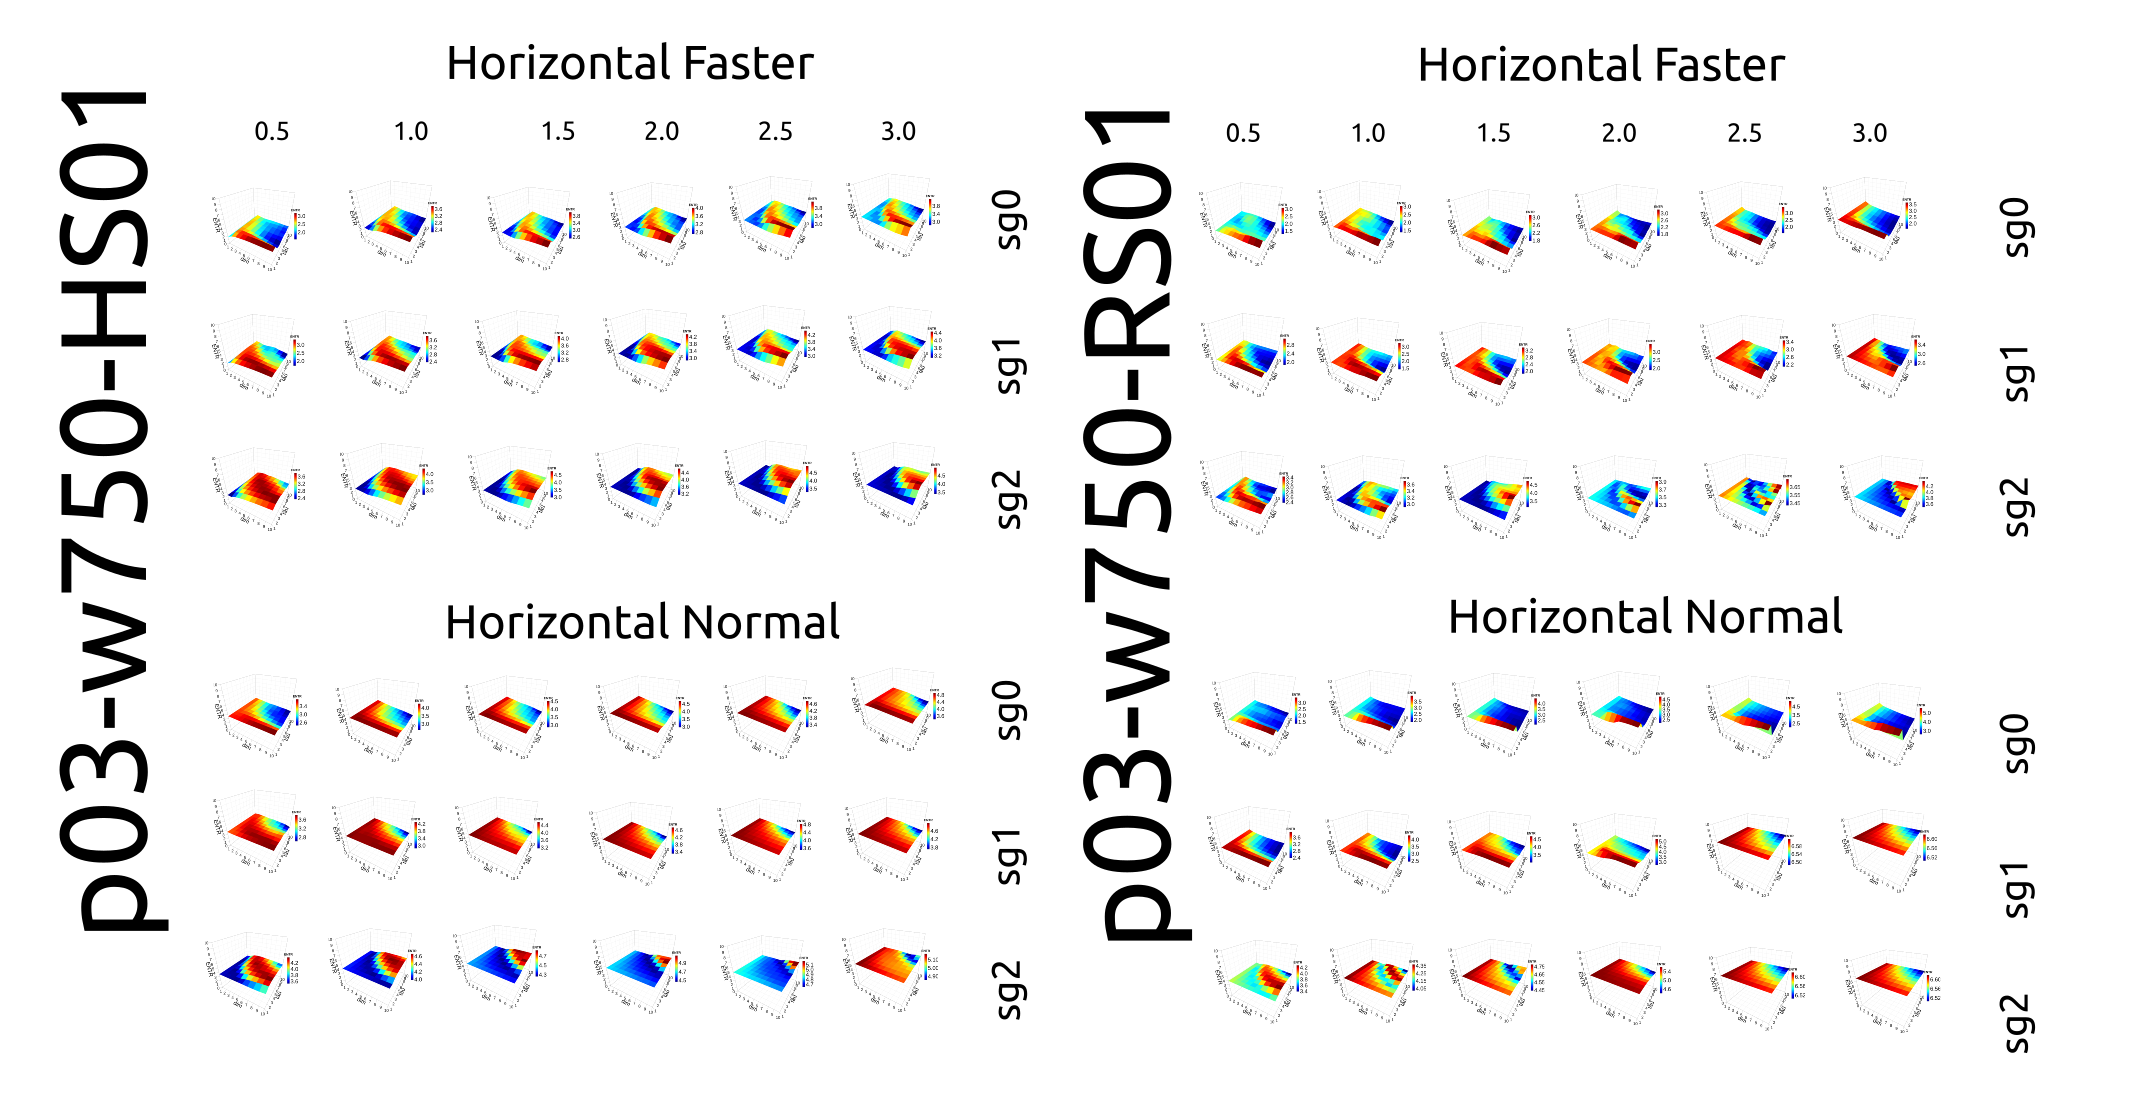
\includegraphics{figures/rqa/output/epsilons/rqa-epsilonsp03w750Horizontal}
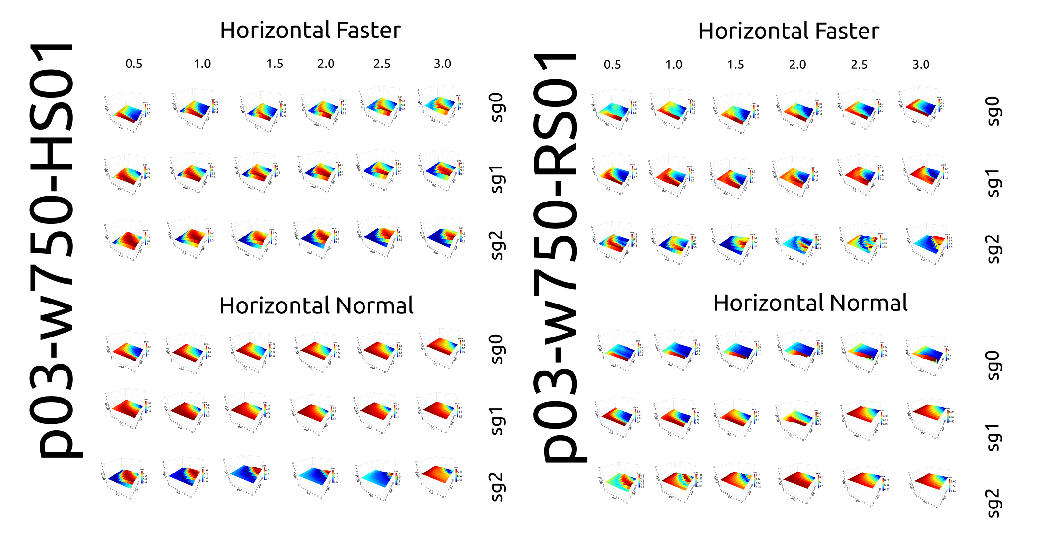
\includegraphics{sm-fig23}
    	\caption{
	{\bf RQA-Entr for participant 03 performing horizontal movements for a window size of 750 samples.}
		%RQA-Entr surface plots are for participant $p03$
		%for horizontal and vertical arm movements in normal
		%and faster velocity (HN, HF, VN, VF)
		%with the normalised GyroZ or GyroY axis
		%((sg0) raw-normalised (sg0zmuv),
		%(sg1) normalised-smoothed 1 and
		%(sg1) normalised-smoothed 2)
		%and with one sensor attached to the participant (HS01)
		%and other sensor attached to the robot (RS01).
	Code and data to reproduce the figure is available in \cite{srep2021}.
        }
    \label{fig-p03-H-w750}
\end{figure}
%---------------------------------(FIGURE)------------------------------------
%---------------------------------FIGURE)-------------------------------------
\begin{figure}[hb!]
\centering
%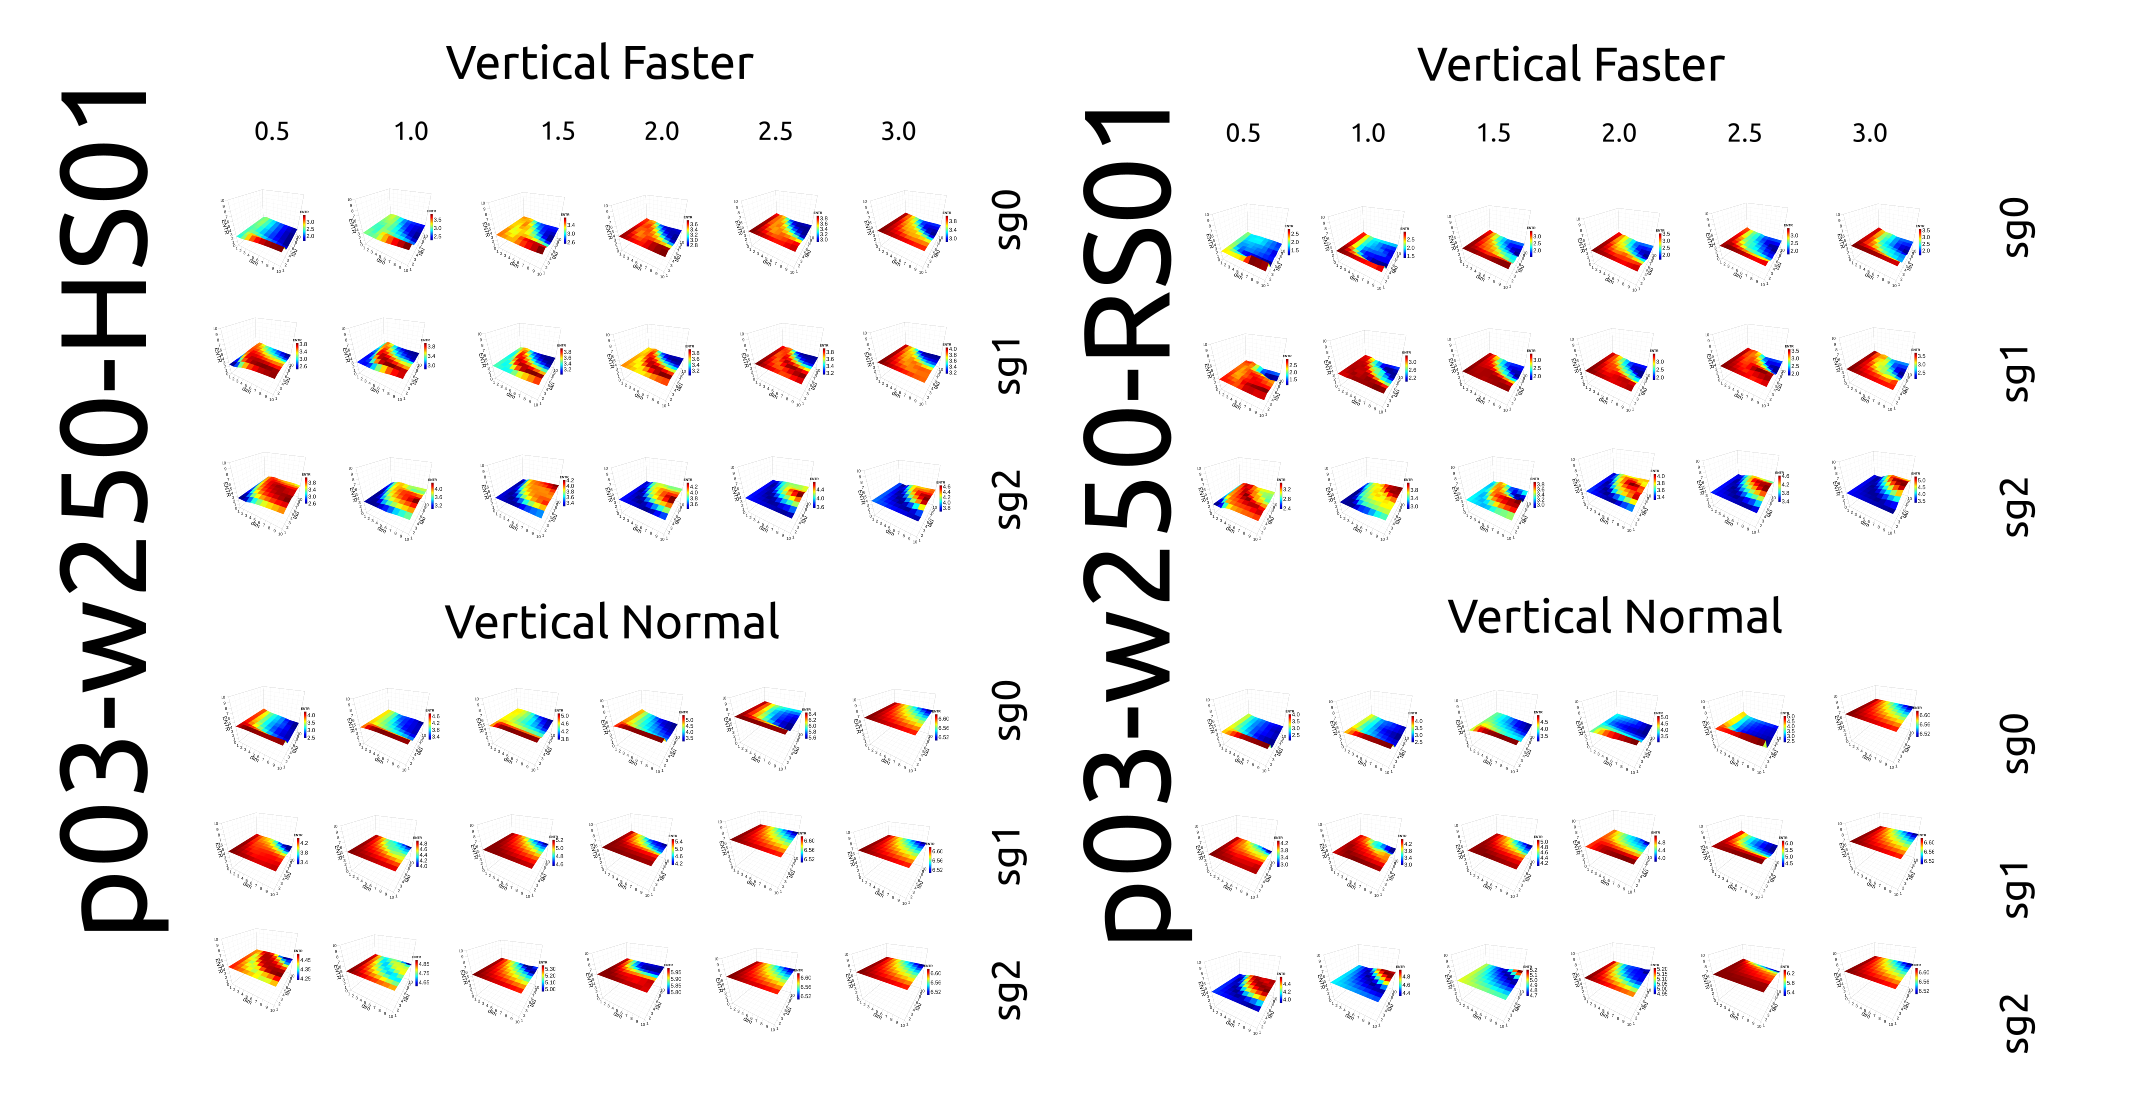
\includegraphics{figures/rqa/output/epsilons/rqa-epsilonsp03w750Vertical}
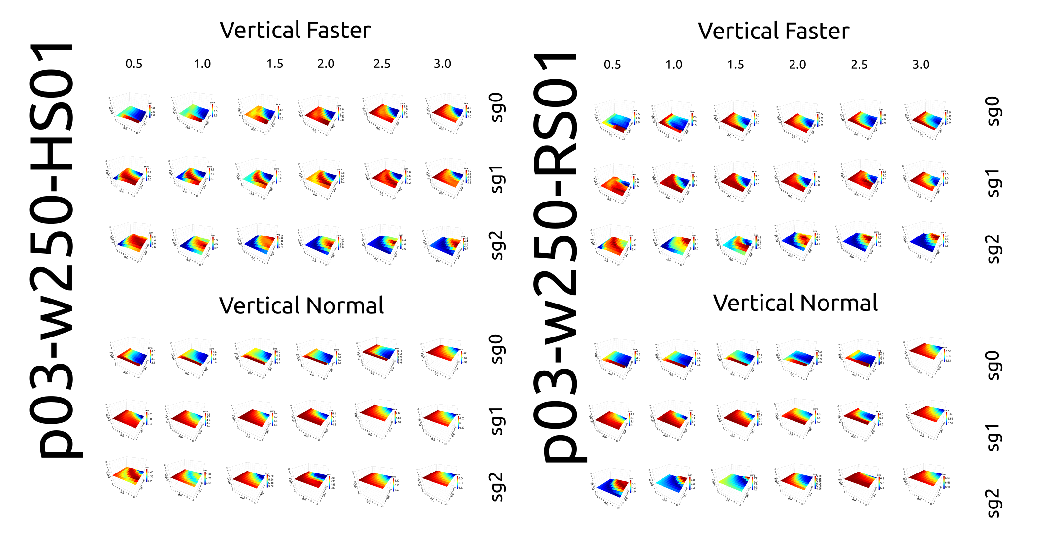
\includegraphics{sm-fig24}
    	\caption{
	{\bf RQA-Entr for participant 03 performing vertical movements for a window size of 750 samples.}
		%RQA-Entr surface plots are for participant $p03$
		%for horizontal and vertical arm movements in normal
		%and faster velocity (HN, HF, VN, VF)
		%with the normalised GyroZ or GyroY axis
		%((sg0) raw-normalised (sg0zmuv),
		%(sg1) normalised-smoothed 1 and
		%(sg1) normalised-smoothed 2)
		%and with one sensor attached to the participant (HS01)
		%and other sensor attached to the robot (RS01).
	Code and data to reproduce the figure is available in \cite{srep2021}.
        }
    \label{fig-p03-V-w750}
\end{figure}
%---------------------------------(FIGURE)------------------------------------



%%
%%%%%%%%%%%%%%%%%%%%%%%%%%%%%%%%%%%%
%%\subsection{Activities and sensors}
%%
%%%%%%%%%%%%%%%%%%%%%%%%%%%%%%%%%%%
%\subsection{Participants}
%%Similarly, 3D surfaces of RQA metrics were also computed for three
%%participants (Fig.~\ref{fig:topo_participants}).
%
%%%%%%%%%%%%%%%%%%%%%%%%%%%%%%%%%%
%\subsection{Window length}
%%RQA metrics are also affected by
%%the window length where for example four window lengths of 100, 250, 500
%%and 750 samples (Fig.~\ref{fig:topo_sensoractivities}).
%


\clearpage
\bibliographystyle{plain}
%\bibliography{../../../../supplementary-material/tex/references}
\documentclass[12pt]{article}
\usepackage[margin=15mm]{geometry}
\usepackage{graphicx}
\usepackage{url}
\graphicspath{{../../}} %%%goes to the path: docs/

\title{
Supplementary Material
}
\author{Miguel Xochicale}
\date{ \today }

\begin{document}
\maketitle

\begin{abstract}
Report for supplementary material where section 1 describes datasets and section 2 shows surface plots of 3D RQA ENTR values for 3 participants (p01, p02 and p03).
\end{abstract}

\tableofcontents
%\newpage


%%%%%%%%%%%%%%%%%%%%%%%%%%%%%%%%%%%%%%%%%%%%%%%%%%%%%%%%%%%%%%
\section{Datasets}
Datasets are for 
(a) window size of 100, 250, 500 and 750 samples (w100, w250, w500, w750);
(b) smoothness: sg0, sg1 and sg2;
(c) movement: Horizontal Normal (HN), Horizontal Faster (HF), Vertical Normal (VN) and Vertical Faster (VF); and 
(d) sensors: Sensor attached to Human (HS01), sensor attached to Robot (RS01).

The location of the dataset is shown below with the first two lines of xdatav00.dt denoting labels.
\begin{verbatim}
~/srep2021/data/dataset$ tree --si
[ 46M]  xdata_v00.dt
.
.
.
"Participant" "Activity" "Sensor" "Sample" "Time" 
"sg0zmuvGyroY" "sg1zmuvGyroY" "sg2zmuvGyroY" 
"sg0zmuvGyroZ" "sg1zmuvGyroZ" "sg2zmuvGyroZ"
...
"p01" "HN" "HS01" 1 0 
0.0110396263359954 0.00606430191548277 0.0385586376765087 
0.00467559072085554 0.00509907428630649 0.168927517477539
...
\end{verbatim}

%├── [4.1k]  dataset
%│   └── [ 46M]  xdata_v00.dt
%.
%.
%.

%%%%%%%%%%%%%%%%%%%%%%%%%%%%%%%%%%%%%%%%%%%%%%%%%%%%%%%%%%%%%%
\section{3D RQA ENTR values}
Location of code, data and figures for 3D RQA ENTR values is shown below 
\begin{verbatim}
## Code
$HOME/srep2021/code/rscripts/G_3Drqa
`> source(  paste( getwd(), '/C_3Drqa_plots_epsilons.R', sep=''), echo=TRUE )`

## Data
$HOME/srep2021/data/rqa$ tree -s 

## Figures
$HOME/srep2021/docs/figures/rqa/src/3drqa_epsilons$ tree -s
\end{verbatim}

For the following plots, datasets for NN participants where NN is 01, 02 and 03 are:
\begin{verbatim}
RQAs_pNNw100.dt
RQAs_pNNw250.dt
RQAs_pNNw500.dt
RQAs_pNNw750.dt
\end{verbatim}


\subsection{Participant 01}
%X Three level of
%X smoothness were computed for RQA metrics showing smoothed 3D surfaces and
%X the level of smoothness increase (Fig.~\ref{fig:topo_smoothness}).
%After data collection, raw time series were windowed, normalised and smoothed. 

Figures \ref{fig-p01-H-w100} and \ref{fig-p01-V-w100} are for a window size of 100 samples.
Figures \ref{fig-p01-H-w250} and \ref{fig-p01-V-w250} are for a window size of 250 samples.
Figures \ref{fig-p01-H-w500} and \ref{fig-p01-V-w500} are for a window size of 500 samples.
Figures \ref{fig-p01-H-w750} and \ref{fig-p01-V-w750} are for a window size of 750 samples.

%we only present 10-sec (500 samples) window length time series for
%three participants (p01, p01 and p03) performing horizontal
%arm movements (axis GyroZ) and vertical arm movements (axis GyroY) (Figs \ref{fig-p01-w100}).

\newpage
%---------------------------------FIGURE)-------------------------------------
\begin{figure}[ht!]
\centering
%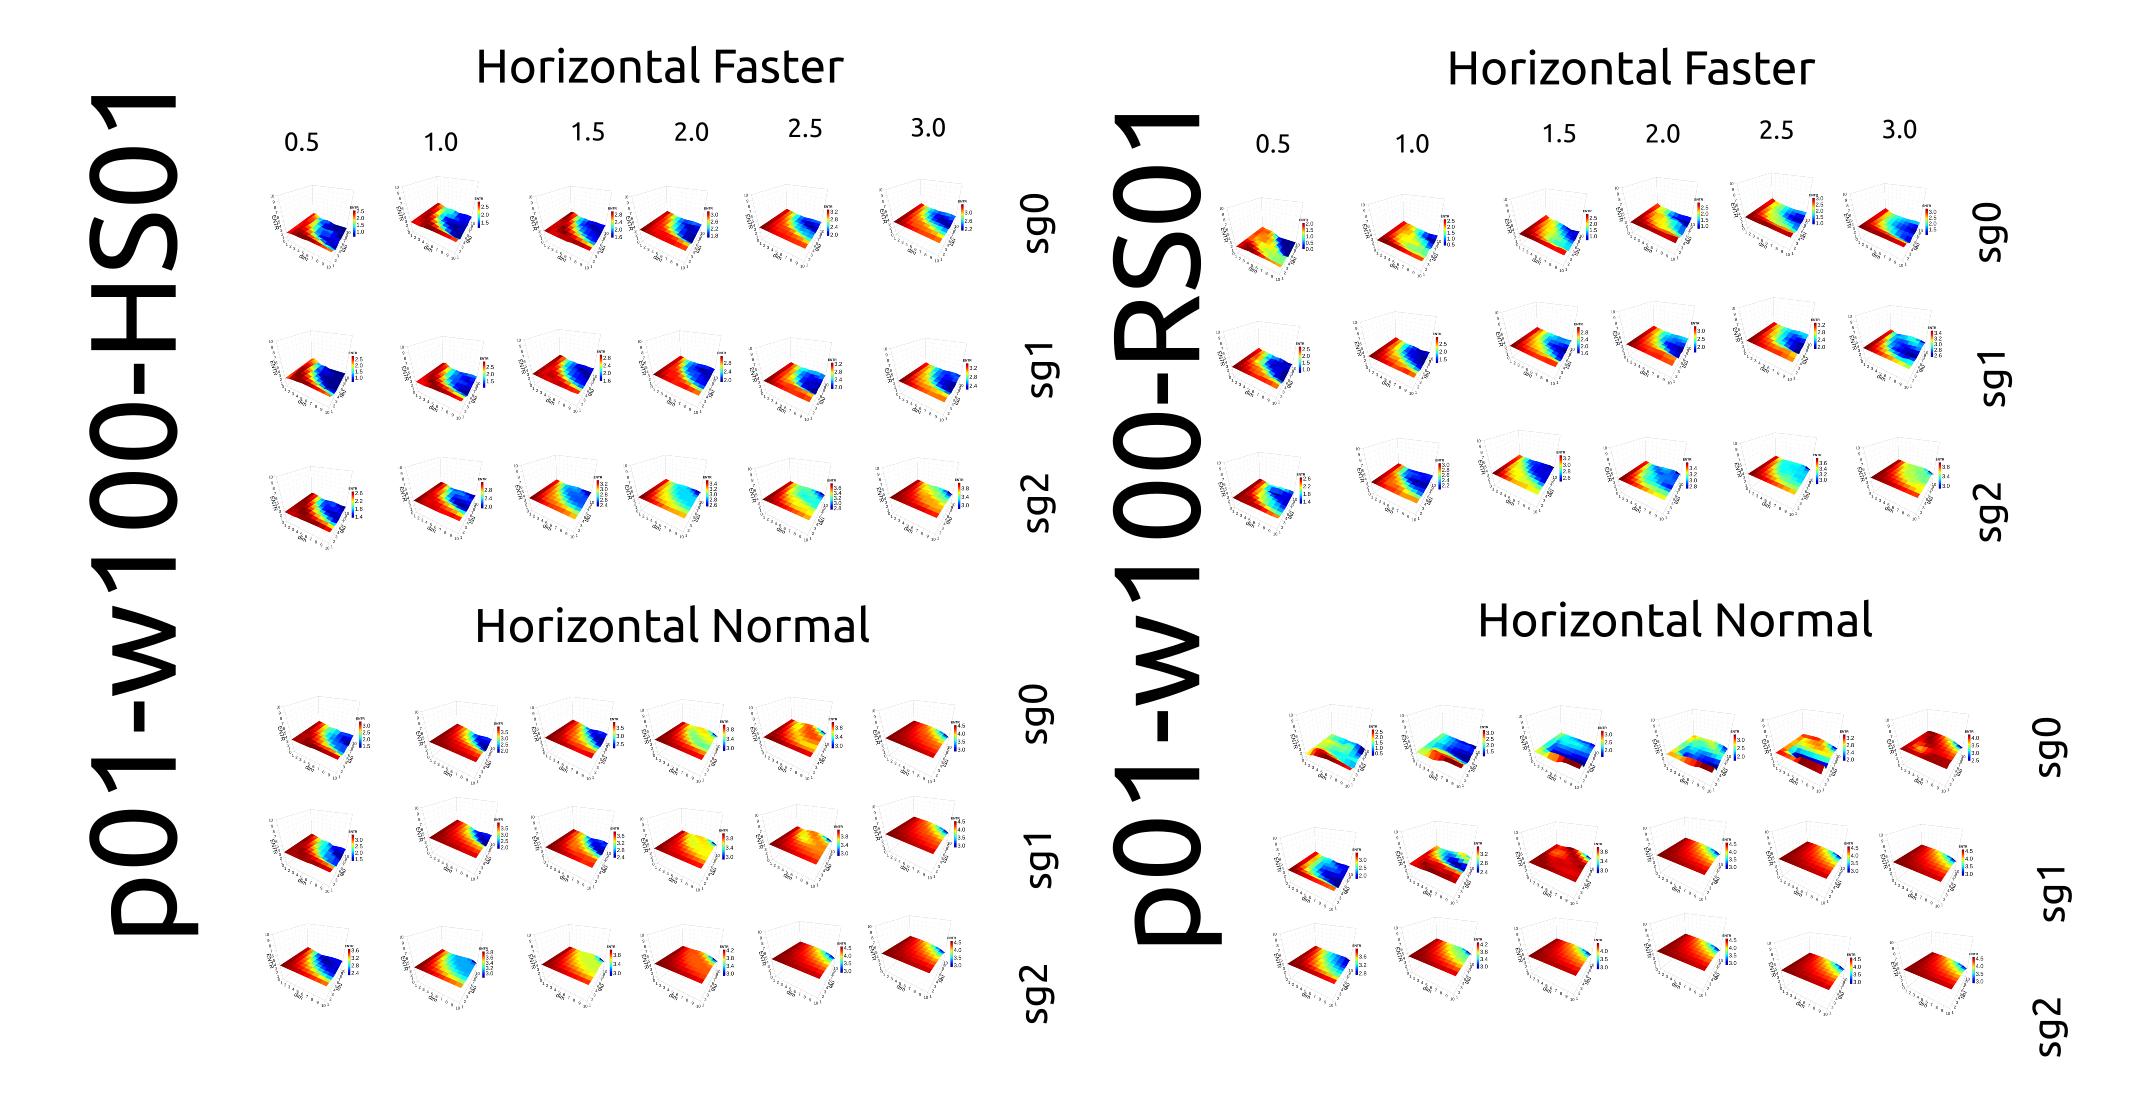
\includegraphics[scale=1.0]{figures/rqa/output/epsilons/rqa-epsilonsp01w100Horizontal}
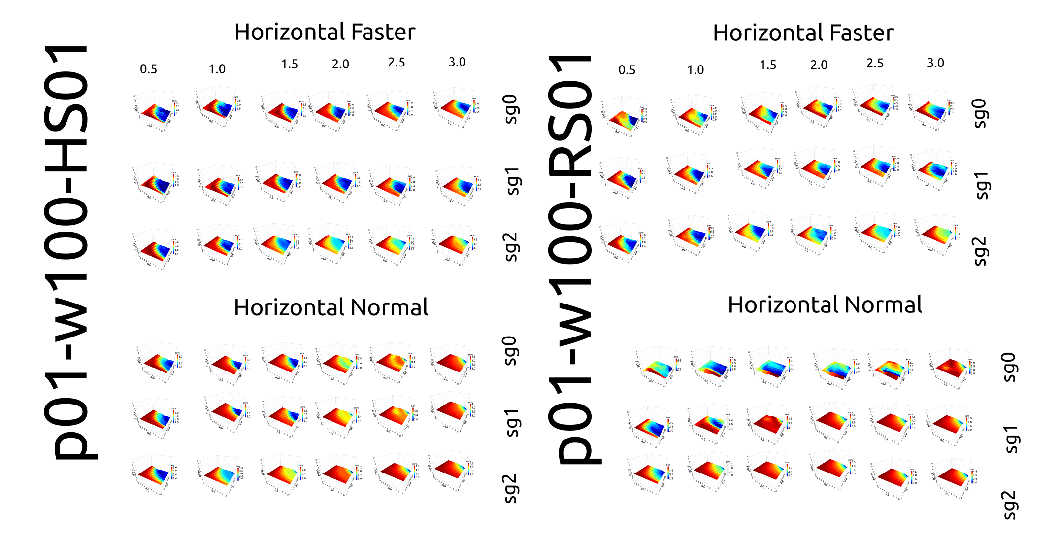
\includegraphics[scale=1.0]{sm-fig01}
    	\caption{
	{\bf RQA-Entr for participant 01 performing horizontal movements for a window size of 100 samples.}
		%RQA-Entr surface plots are for participant $p01$
		%for horizontal and vertical arm movements in normal
		%and faster velocity (HN, HF, VN, VF)
		%with the normalised GyroZ or GyroY axis
		%((sg0) raw-normalised (sg0zmuv),
		%(sg1) normalised-smoothed 1 and
		%(sg1) normalised-smoothed 2)
		%and with one sensor attached to the participant (HS01)
		%and other sensor attached to the robot (RS01).
	Code and data to reproduce the figure is available in \cite{srep2021}.
        }
    \label{fig-p01-H-w100}
\end{figure}
%---------------------------------(FIGURE)------------------------------------
%---------------------------------FIGURE)-------------------------------------
\begin{figure}[hb!]
\centering
%\includegraphics[scale=1.0]{figures/rqa/output/epsilons/rqa-epsilonsp01w100Vertical}
\includegraphics[scale=1.0]{sm-fig02}
    	\caption{
	{\bf RQA-Entr for participant 01 performing vertical movements for a window size of 100 samples.}
		%RQA-Entr surface plots are for participant $p01$
		%for horizontal and vertical arm movements in normal
		%and faster velocity (HN, HF, VN, VF)
		%with the normalised GyroZ or GyroY axis
		%((sg0) raw-normalised (sg0zmuv),
		%(sg1) normalised-smoothed 1 and
		%(sg1) normalised-smoothed 2)
		%and with one sensor attached to the participant (HS01)
		%and other sensor attached to the robot (RS01).
	Code and data to reproduce the figure is available in \cite{srep2021}.
        }
    \label{fig-p01-V-w100}
\end{figure}
%---------------------------------(FIGURE)------------------------------------


\newpage
%---------------------------------FIGURE)-------------------------------------
\begin{figure}[ht!]
\centering
%\includegraphics{figures/rqa/output/epsilons/rqa-epsilonsp01w250Horizontal}
\includegraphics{sm-fig03}
    	\caption{
	{\bf RQA-Entr for participant 01 performing horizontal movements for a window size of 250 samples.}
		%RQA-Entr surface plots are for participant $p01$
		%for horizontal and vertical arm movements in normal
		%and faster velocity (HN, HF, VN, VF)
		%with the normalised GyroZ or GyroY axis
		%((sg0) raw-normalised (sg0zmuv),
		%(sg1) normalised-smoothed 1 and
		%(sg1) normalised-smoothed 2)
		%and with one sensor attached to the participant (HS01)
		%and other sensor attached to the robot (RS01).
	Code and data to reproduce the figure is available in \cite{srep2021}.
        }
    \label{fig-p01-H-w250}
\end{figure}
%---------------------------------(FIGURE)------------------------------------
%---------------------------------FIGURE)-------------------------------------
\begin{figure}[hb!]
\centering
%\includegraphics{figures/rqa/output/epsilons/rqa-epsilonsp01w250Vertical}
\includegraphics{sm-fig04}
    	\caption{
	{\bf RQA-Entr for participant 01 performing vertical movements for a window size of 250 samples.}
		%RQA-Entr surface plots are for participant $p01$
		%for horizontal and vertical arm movements in normal
		%and faster velocity (HN, HF, VN, VF)
		%with the normalised GyroZ or GyroY axis
		%((sg0) raw-normalised (sg0zmuv),
		%(sg1) normalised-smoothed 1 and
		%(sg1) normalised-smoothed 2)
		%and with one sensor attached to the participant (HS01)
		%and other sensor attached to the robot (RS01).
	Code and data to reproduce the figure is available in \cite{srep2021}.
        }
    \label{fig-p01-V-w250}
\end{figure}
%---------------------------------(FIGURE)------------------------------------


\newpage
%---------------------------------FIGURE)-------------------------------------
\begin{figure}[ht!]
\centering
%\includegraphics{figures/rqa/output/epsilons/rqa-epsilonsp01w500Horizontal}
\includegraphics{sm-fig05}
    	\caption{
	{\bf RQA-Entr for participant 01 performing horizontal movements for a window size of 500 samples.}
		%RQA-Entr surface plots are for participant $p01$
		%for horizontal and vertical arm movements in normal
		%and faster velocity (HN, HF, VN, VF)
		%with the normalised GyroZ or GyroY axis
		%((sg0) raw-normalised (sg0zmuv),
		%(sg1) normalised-smoothed 1 and
		%(sg1) normalised-smoothed 2)
		%and with one sensor attached to the participant (HS01)
		%and other sensor attached to the robot (RS01).
	Code and data to reproduce the figure is available in \cite{srep2021}.
        }
    \label{fig-p01-H-w500}
\end{figure}
%---------------------------------(FIGURE)------------------------------------
%---------------------------------FIGURE)-------------------------------------
\begin{figure}[hb!]
\centering
%\includegraphics{figures/rqa/output/epsilons/rqa-epsilonsp01w500Vertical}
\includegraphics{sm-fig06}
    	\caption{
	{\bf RQA-Entr for participant 01 performing vertical movements for a window size of 500 samples.}
		%RQA-Entr surface plots are for participant $p01$
		%for horizontal and vertical arm movements in normal
		%and faster velocity (HN, HF, VN, VF)
		%with the normalised GyroZ or GyroY axis
		%((sg0) raw-normalised (sg0zmuv),
		%(sg1) normalised-smoothed 1 and
		%(sg1) normalised-smoothed 2)
		%and with one sensor attached to the participant (HS01)
		%and other sensor attached to the robot (RS01).
	Code and data to reproduce the figure is available in \cite{srep2021}.
        }
    \label{fig-p01-V-w500}
\end{figure}
%---------------------------------(FIGURE)------------------------------------


\newpage
%---------------------------------FIGURE)-------------------------------------
\begin{figure}[ht!]
\centering
%\includegraphics{figures/rqa/output/epsilons/rqa-epsilonsp01w750Horizontal}
\includegraphics{sm-fig07}
    	\caption{
	{\bf RQA-Entr for participant 01 performing horizontal movements for a window size of 750 samples.}
		%RQA-Entr surface plots are for participant $p01$
		%for horizontal and vertical arm movements in normal
		%and faster velocity (HN, HF, VN, VF)
		%with the normalised GyroZ or GyroY axis
		%((sg0) raw-normalised (sg0zmuv),
		%(sg1) normalised-smoothed 1 and
		%(sg1) normalised-smoothed 2)
		%and with one sensor attached to the participant (HS01)
		%and other sensor attached to the robot (RS01).
	Code and data to reproduce the figure is available in \cite{srep2021}.
        }
    \label{fig-p01-H-w750}
\end{figure}
%---------------------------------(FIGURE)------------------------------------
%---------------------------------FIGURE)-------------------------------------
\begin{figure}[hb!]
\centering
%\includegraphics{figures/rqa/output/epsilons/rqa-epsilonsp01w750Vertical}
\includegraphics{sm-fig08}
    	\caption{
	{\bf RQA-Entr for participant 01 performing vertical movements for a window size of 750 samples.}
		%RQA-Entr surface plots are for participant $p01$
		%for horizontal and vertical arm movements in normal
		%and faster velocity (HN, HF, VN, VF)
		%with the normalised GyroZ or GyroY axis
		%((sg0) raw-normalised (sg0zmuv),
		%(sg1) normalised-smoothed 1 and
		%(sg1) normalised-smoothed 2)
		%and with one sensor attached to the participant (HS01)
		%and other sensor attached to the robot (RS01).
	Code and data to reproduce the figure is available in \cite{srep2021}.
        }
    \label{fig-p01-V-w750}
\end{figure}
%---------------------------------(FIGURE)------------------------------------






\newpage
\subsection{Participant 02}
%X Three level of
%X smoothness were computed for RQA metrics showing smoothed 3D surfaces and
%X the level of smoothness increase (Fig.~\ref{fig:topo_smoothness}).
%After data collection, raw time series were windowed, normalised and
%smoothed. Then, due to space limitations and to have simple visualisation,
Figures \ref{fig-p02-H-w100} and \ref{fig-p02-V-w100} are for a window size of 100 samples.
Figures \ref{fig-p02-H-w250} and \ref{fig-p02-V-w250} are for a window size of 250 samples.
Figures \ref{fig-p02-H-w500} and \ref{fig-p02-V-w500} are for a window size of 500 samples.
Figures \ref{fig-p02-H-w750} and \ref{fig-p02-V-w750} are for a window size of 750 samples.

\newpage
%---------------------------------FIGURE)-------------------------------------
\begin{figure}[ht!]
\centering
%\includegraphics[scale=1.0]{figures/rqa/output/epsilons/rqa-epsilonsp02w100Horizontal}
\includegraphics[scale=1.0]{sm-fig09}
    	\caption{
	{\bf RQA-Entr for participant 02 performing horizontal movements for a window size of 100 samples.}
		%RQA-Entr surface plots are for participant $p02$
		%for horizontal and vertical arm movements in normal
		%and faster velocity (HN, HF, VN, VF)
		%with the normalised GyroZ or GyroY axis
		%((sg0) raw-normalised (sg0zmuv),
		%(sg1) normalised-smoothed 1 and
		%(sg1) normalised-smoothed 2)
		%and with one sensor attached to the participant (HS01)
		%and other sensor attached to the robot (RS01).
	Code and data to reproduce the figure is available in \cite{srep2021}.
        }
    \label{fig-p02-H-w100}
\end{figure}
%---------------------------------(FIGURE)------------------------------------
%---------------------------------FIGURE)-------------------------------------
\begin{figure}[hb!]
\centering
%\includegraphics[scale=1.0]{figures/rqa/output/epsilons/rqa-epsilonsp02w100Vertical}
\includegraphics[scale=1.0]{sm-fig10}
    	\caption{
	{\bf RQA-Entr for participant 02 performing vertical movements for a window size of 100 samples.}
		%RQA-Entr surface plots are for participant $p02$
		%for horizontal and vertical arm movements in normal
		%and faster velocity (HN, HF, VN, VF)
		%with the normalised GyroZ or GyroY axis
		%((sg0) raw-normalised (sg0zmuv),
		%(sg1) normalised-smoothed 1 and
		%(sg1) normalised-smoothed 2)
		%and with one sensor attached to the participant (HS01)
		%and other sensor attached to the robot (RS01).
	Code and data to reproduce the figure is available in \cite{srep2021}.
        }
    \label{fig-p02-V-w100}
\end{figure}
%---------------------------------(FIGURE)------------------------------------


\newpage
%---------------------------------FIGURE)-------------------------------------
\begin{figure}[ht!]
\centering
%\includegraphics{figures/rqa/output/epsilons/rqa-epsilonsp02w250Horizontal}
\includegraphics{sm-fig11}
    	\caption{
	{\bf RQA-Entr for participant 02 performing horizontal movements for a window size of 250 samples.}
		%RQA-Entr surface plots are for participant $p02$
		%for horizontal and vertical arm movements in normal
		%and faster velocity (HN, HF, VN, VF)
		%with the normalised GyroZ or GyroY axis
		%((sg0) raw-normalised (sg0zmuv),
		%(sg1) normalised-smoothed 1 and
		%(sg1) normalised-smoothed 2)
		%and with one sensor attached to the participant (HS01)
		%and other sensor attached to the robot (RS01).
	Code and data to reproduce the figure is available in \cite{srep2021}.
        }
    \label{fig-p02-H-w250}
\end{figure}
%---------------------------------(FIGURE)------------------------------------
%---------------------------------FIGURE)-------------------------------------
\begin{figure}[hb!]
\centering
%\includegraphics{figures/rqa/output/epsilons/rqa-epsilonsp02w250Vertical}
\includegraphics{sm-fig12}
    	\caption{
	{\bf RQA-Entr for participant 02 performing vertical movements for a window size of 250 samples.}
		%RQA-Entr surface plots are for participant $p02$
		%for horizontal and vertical arm movements in normal
		%and faster velocity (HN, HF, VN, VF)
		%with the normalised GyroZ or GyroY axis
		%((sg0) raw-normalised (sg0zmuv),
		%(sg1) normalised-smoothed 1 and
		%(sg1) normalised-smoothed 2)
		%and with one sensor attached to the participant (HS01)
		%and other sensor attached to the robot (RS01).
	Code and data to reproduce the figure is available in \cite{srep2021}.
        }
    \label{fig-p02-V-w250}
\end{figure}
%---------------------------------(FIGURE)------------------------------------


\newpage
%---------------------------------FIGURE)-------------------------------------
\begin{figure}[ht!]
\centering
%\includegraphics{figures/rqa/output/epsilons/rqa-epsilonsp02w500Horizontal}
\includegraphics{sm-fig13}
    	\caption{
	{\bf RQA-Entr for participant 02 performing horizontal movements for a window size of 500 samples.}
		%RQA-Entr surface plots are for participant $p02$
		%for horizontal and vertical arm movements in normal
		%and faster velocity (HN, HF, VN, VF)
		%with the normalised GyroZ or GyroY axis
		%((sg0) raw-normalised (sg0zmuv),
		%(sg1) normalised-smoothed 1 and
		%(sg1) normalised-smoothed 2)
		%and with one sensor attached to the participant (HS01)
		%and other sensor attached to the robot (RS01).
	Code and data to reproduce the figure is available in \cite{srep2021}.
        }
    \label{fig-p02-H-w500}
\end{figure}
%---------------------------------(FIGURE)------------------------------------
%---------------------------------FIGURE)-------------------------------------
\begin{figure}[hb!]
\centering
%\includegraphics{figures/rqa/output/epsilons/rqa-epsilonsp02w500Vertical}
\includegraphics{sm-fig14}
    	\caption{
	{\bf RQA-Entr for participant 02 performing vertical movements for a window size of 500 samples.}
		%RQA-Entr surface plots are for participant $p02$
		%for horizontal and vertical arm movements in normal
		%and faster velocity (HN, HF, VN, VF)
		%with the normalised GyroZ or GyroY axis
		%((sg0) raw-normalised (sg0zmuv),
		%(sg1) normalised-smoothed 1 and
		%(sg1) normalised-smoothed 2)
		%and with one sensor attached to the participant (HS01)
		%and other sensor attached to the robot (RS01).
	Code and data to reproduce the figure is available in \cite{srep2021}.
        }
    \label{fig-p02-V-w500}
\end{figure}
%---------------------------------(FIGURE)------------------------------------


\newpage
%---------------------------------FIGURE)-------------------------------------
\begin{figure}[ht!]
\centering
%\includegraphics{figures/rqa/output/epsilons/rqa-epsilonsp02w750Horizontal}
\includegraphics{sm-fig15}
    	\caption{
	{\bf RQA-Entr for participant 02 performing horizontal movements for a window size of 750 samples.}
		%RQA-Entr surface plots are for participant $p02$
		%for horizontal and vertical arm movements in normal
		%and faster velocity (HN, HF, VN, VF)
		%with the normalised GyroZ or GyroY axis
		%((sg0) raw-normalised (sg0zmuv),
		%(sg1) normalised-smoothed 1 and
		%(sg1) normalised-smoothed 2)
		%and with one sensor attached to the participant (HS01)
		%and other sensor attached to the robot (RS01).
	Code and data to reproduce the figure is available in \cite{srep2021}.
        }
    \label{fig-p02-H-w750}
\end{figure}
%---------------------------------(FIGURE)------------------------------------
%---------------------------------FIGURE)-------------------------------------
\begin{figure}[hb!]
\centering
%\includegraphics{figures/rqa/output/epsilons/rqa-epsilonsp02w750Vertical}
\includegraphics{sm-fig16}
    	\caption{
	{\bf RQA-Entr for participant 02 performing vertical movements for a window size of 750 samples.}
		%RQA-Entr surface plots are for participant $p02$
		%for horizontal and vertical arm movements in normal
		%and faster velocity (HN, HF, VN, VF)
		%with the normalised GyroZ or GyroY axis
		%((sg0) raw-normalised (sg0zmuv),
		%(sg1) normalised-smoothed 1 and
		%(sg1) normalised-smoothed 2)
		%and with one sensor attached to the participant (HS01)
		%and other sensor attached to the robot (RS01).
	Code and data to reproduce the figure is available in \cite{srep2021}.
        }
    \label{fig-p02-V-w750}
\end{figure}
%---------------------------------(FIGURE)------------------------------------


\newpage
\subsection{Participant 03}
%X Three level of
%X smoothness were computed for RQA metrics showing smoothed 3D surfaces and
%X the level of smoothness increase (Fig.~\ref{fig:topo_smoothness}).
%After data collection, raw time series were windowed, normalised and
%smoothed. Then, due to space limitations and to have simple visualisation,
Figures \ref{fig-p03-H-w100} and \ref{fig-p03-V-w100} are for a window size of 100 samples.
Figures \ref{fig-p03-H-w250} and \ref{fig-p03-V-w250} are for a window size of 250 samples.
Figures \ref{fig-p03-H-w500} and \ref{fig-p03-V-w500} are for a window size of 500 samples.
Figures \ref{fig-p03-H-w750} and \ref{fig-p03-V-w750} are for a window size of 750 samples.


\newpage
%---------------------------------FIGURE)-------------------------------------
\begin{figure}[ht!]
\centering
%\includegraphics[scale=1.0]{figures/rqa/output/epsilons/rqa-epsilonsp03w100Horizontal}
\includegraphics[scale=1.0]{sm-fig17}
    	\caption{
	{\bf RQA-Entr for participant 03 performing horizontal movements for a window size of 100 samples.}
		%RQA-Entr surface plots are for participant $p03$
		%for horizontal and vertical arm movements in normal
		%and faster velocity (HN, HF, VN, VF)
		%with the normalised GyroZ or GyroY axis
		%((sg0) raw-normalised (sg0zmuv),
		%(sg1) normalised-smoothed 1 and
		%(sg1) normalised-smoothed 2)
		%and with one sensor attached to the participant (HS01)
		%and other sensor attached to the robot (RS01).
	Code and data to reproduce the figure is available in \cite{srep2021}.
        }
    \label{fig-p03-H-w100}
\end{figure}
%---------------------------------(FIGURE)------------------------------------
%---------------------------------FIGURE)-------------------------------------
\begin{figure}[hb!]
\centering
%\includegraphics[scale=1.0]{figures/rqa/output/epsilons/rqa-epsilonsp03w100Vertical}
\includegraphics[scale=1.0]{sm-fig18}
    	\caption{
	{\bf RQA-Entr for participant 03 performing vertical movements for a window size of 100 samples.}
		%RQA-Entr surface plots are for participant $p03$
		%for horizontal and vertical arm movements in normal
		%and faster velocity (HN, HF, VN, VF)
		%with the normalised GyroZ or GyroY axis
		%((sg0) raw-normalised (sg0zmuv),
		%(sg1) normalised-smoothed 1 and
		%(sg1) normalised-smoothed 2)
		%and with one sensor attached to the participant (HS01)
		%and other sensor attached to the robot (RS01).
	Code and data to reproduce the figure is available in \cite{srep2021}.
        }
    \label{fig-p03-V-w100}
\end{figure}
%---------------------------------(FIGURE)------------------------------------


\newpage
%---------------------------------FIGURE)-------------------------------------
\begin{figure}[ht!]
\centering
%\includegraphics{figures/rqa/output/epsilons/rqa-epsilonsp03w250Horizontal}
\includegraphics{sm-fig19}
    	\caption{
	{\bf RQA-Entr for participant 03 performing horizontal movements for a window size of 250 samples.}
		%RQA-Entr surface plots are for participant $p03$
		%for horizontal and vertical arm movements in normal
		%and faster velocity (HN, HF, VN, VF)
		%with the normalised GyroZ or GyroY axis
		%((sg0) raw-normalised (sg0zmuv),
		%(sg1) normalised-smoothed 1 and
		%(sg1) normalised-smoothed 2)
		%and with one sensor attached to the participant (HS01)
		%and other sensor attached to the robot (RS01).
	Code and data to reproduce the figure is available in \cite{srep2021}.
        }
    \label{fig-p03-H-w250}
\end{figure}
%---------------------------------(FIGURE)------------------------------------
%---------------------------------FIGURE)-------------------------------------
\begin{figure}[hb!]
\centering
%\includegraphics{figures/rqa/output/epsilons/rqa-epsilonsp03w250Vertical}
\includegraphics{sm-fig20}
    	\caption{
	{\bf RQA-Entr for participant 03 performing vertical movements for a window size of 250 samples.}
		%RQA-Entr surface plots are for participant $p03$
		%for horizontal and vertical arm movements in normal
		%and faster velocity (HN, HF, VN, VF)
		%with the normalised GyroZ or GyroY axis
		%((sg0) raw-normalised (sg0zmuv),
		%(sg1) normalised-smoothed 1 and
		%(sg1) normalised-smoothed 2)
		%and with one sensor attached to the participant (HS01)
		%and other sensor attached to the robot (RS01).
	Code and data to reproduce the figure is available in \cite{srep2021}.
        }
    \label{fig-p03-V-w250}
\end{figure}
%---------------------------------(FIGURE)------------------------------------


\newpage
%---------------------------------FIGURE)-------------------------------------
\begin{figure}[ht!]
\centering
%\includegraphics{figures/rqa/output/epsilons/rqa-epsilonsp03w500Horizontal}
\includegraphics{sm-fig21}
    	\caption{
	{\bf RQA-Entr for participant 03 performing horizontal movements for a window size of 500 samples.}
		%RQA-Entr surface plots are for participant $p03$
		%for horizontal and vertical arm movements in normal
		%and faster velocity (HN, HF, VN, VF)
		%with the normalised GyroZ or GyroY axis
		%((sg0) raw-normalised (sg0zmuv),
		%(sg1) normalised-smoothed 1 and
		%(sg1) normalised-smoothed 2)
		%and with one sensor attached to the participant (HS01)
		%and other sensor attached to the robot (RS01).
	Code and data to reproduce the figure is available in \cite{srep2021}.
        }
    \label{fig-p03-H-w500}
\end{figure}
%---------------------------------(FIGURE)------------------------------------
%---------------------------------FIGURE)-------------------------------------
\begin{figure}[hb!]
\centering
%\includegraphics{figures/rqa/output/epsilons/rqa-epsilonsp03w500Vertical}
\includegraphics{sm-fig22}
    	\caption{
	{\bf RQA-Entr for participant 03 performing vertical movements for a window size of 500 samples.}
		%RQA-Entr surface plots are for participant $p03$
		%for horizontal and vertical arm movements in normal
		%and faster velocity (HN, HF, VN, VF)
		%with the normalised GyroZ or GyroY axis
		%((sg0) raw-normalised (sg0zmuv),
		%(sg1) normalised-smoothed 1 and
		%(sg1) normalised-smoothed 2)
		%and with one sensor attached to the participant (HS01)
		%and other sensor attached to the robot (RS01).
	Code and data to reproduce the figure is available in \cite{srep2021}.
        }
    \label{fig-p03-V-w500}
\end{figure}
%---------------------------------(FIGURE)------------------------------------


\newpage
%---------------------------------FIGURE)-------------------------------------
\begin{figure}[ht!]
\centering
%\includegraphics{figures/rqa/output/epsilons/rqa-epsilonsp03w750Horizontal}
\includegraphics{sm-fig23}
    	\caption{
	{\bf RQA-Entr for participant 03 performing horizontal movements for a window size of 750 samples.}
		%RQA-Entr surface plots are for participant $p03$
		%for horizontal and vertical arm movements in normal
		%and faster velocity (HN, HF, VN, VF)
		%with the normalised GyroZ or GyroY axis
		%((sg0) raw-normalised (sg0zmuv),
		%(sg1) normalised-smoothed 1 and
		%(sg1) normalised-smoothed 2)
		%and with one sensor attached to the participant (HS01)
		%and other sensor attached to the robot (RS01).
	Code and data to reproduce the figure is available in \cite{srep2021}.
        }
    \label{fig-p03-H-w750}
\end{figure}
%---------------------------------(FIGURE)------------------------------------
%---------------------------------FIGURE)-------------------------------------
\begin{figure}[hb!]
\centering
%\includegraphics{figures/rqa/output/epsilons/rqa-epsilonsp03w750Vertical}
\includegraphics{sm-fig24}
    	\caption{
	{\bf RQA-Entr for participant 03 performing vertical movements for a window size of 750 samples.}
		%RQA-Entr surface plots are for participant $p03$
		%for horizontal and vertical arm movements in normal
		%and faster velocity (HN, HF, VN, VF)
		%with the normalised GyroZ or GyroY axis
		%((sg0) raw-normalised (sg0zmuv),
		%(sg1) normalised-smoothed 1 and
		%(sg1) normalised-smoothed 2)
		%and with one sensor attached to the participant (HS01)
		%and other sensor attached to the robot (RS01).
	Code and data to reproduce the figure is available in \cite{srep2021}.
        }
    \label{fig-p03-V-w750}
\end{figure}
%---------------------------------(FIGURE)------------------------------------



%%
%%%%%%%%%%%%%%%%%%%%%%%%%%%%%%%%%%%%
%%\subsection{Activities and sensors}
%%
%%%%%%%%%%%%%%%%%%%%%%%%%%%%%%%%%%%
%\subsection{Participants}
%%Similarly, 3D surfaces of RQA metrics were also computed for three
%%participants (Fig.~\ref{fig:topo_participants}).
%
%%%%%%%%%%%%%%%%%%%%%%%%%%%%%%%%%%
%\subsection{Window length}
%%RQA metrics are also affected by
%%the window length where for example four window lengths of 100, 250, 500
%%and 750 samples (Fig.~\ref{fig:topo_sensoractivities}).
%


\clearpage
\bibliographystyle{plain}
%\bibliography{../../../../supplementary-material/tex/references}
\documentclass[12pt]{article}
\usepackage[margin=15mm]{geometry}
\usepackage{graphicx}
\usepackage{url}
\graphicspath{{../../}} %%%goes to the path: docs/

\title{
Supplementary Material
}
\author{Miguel Xochicale}
\date{ \today }

\begin{document}
\maketitle

\begin{abstract}
Report for supplementary material where section 1 describes datasets and section 2 shows surface plots of 3D RQA ENTR values for 3 participants (p01, p02 and p03).
\end{abstract}

\tableofcontents
%\newpage


%%%%%%%%%%%%%%%%%%%%%%%%%%%%%%%%%%%%%%%%%%%%%%%%%%%%%%%%%%%%%%
\section{Datasets}
Datasets are for 
(a) window size of 100, 250, 500 and 750 samples (w100, w250, w500, w750);
(b) smoothness: sg0, sg1 and sg2;
(c) movement: Horizontal Normal (HN), Horizontal Faster (HF), Vertical Normal (VN) and Vertical Faster (VF); and 
(d) sensors: Sensor attached to Human (HS01), sensor attached to Robot (RS01).

The location of the dataset is shown below with the first two lines of xdatav00.dt denoting labels.
\begin{verbatim}
~/srep2021/data/dataset$ tree --si
[ 46M]  xdata_v00.dt
.
.
.
"Participant" "Activity" "Sensor" "Sample" "Time" 
"sg0zmuvGyroY" "sg1zmuvGyroY" "sg2zmuvGyroY" 
"sg0zmuvGyroZ" "sg1zmuvGyroZ" "sg2zmuvGyroZ"
...
"p01" "HN" "HS01" 1 0 
0.0110396263359954 0.00606430191548277 0.0385586376765087 
0.00467559072085554 0.00509907428630649 0.168927517477539
...
\end{verbatim}

%├── [4.1k]  dataset
%│   └── [ 46M]  xdata_v00.dt
%.
%.
%.

%%%%%%%%%%%%%%%%%%%%%%%%%%%%%%%%%%%%%%%%%%%%%%%%%%%%%%%%%%%%%%
\section{3D RQA ENTR values}
Location of code, data and figures for 3D RQA ENTR values is shown below 
\begin{verbatim}
## Code
$HOME/srep2021/code/rscripts/G_3Drqa
`> source(  paste( getwd(), '/C_3Drqa_plots_epsilons.R', sep=''), echo=TRUE )`

## Data
$HOME/srep2021/data/rqa$ tree -s 

## Figures
$HOME/srep2021/docs/figures/rqa/src/3drqa_epsilons$ tree -s
\end{verbatim}

For the following plots, datasets for NN participants where NN is 01, 02 and 03 are:
\begin{verbatim}
RQAs_pNNw100.dt
RQAs_pNNw250.dt
RQAs_pNNw500.dt
RQAs_pNNw750.dt
\end{verbatim}


\subsection{Participant 01}
%X Three level of
%X smoothness were computed for RQA metrics showing smoothed 3D surfaces and
%X the level of smoothness increase (Fig.~\ref{fig:topo_smoothness}).
%After data collection, raw time series were windowed, normalised and smoothed. 

Figures \ref{fig-p01-H-w100} and \ref{fig-p01-V-w100} are for a window size of 100 samples.
Figures \ref{fig-p01-H-w250} and \ref{fig-p01-V-w250} are for a window size of 250 samples.
Figures \ref{fig-p01-H-w500} and \ref{fig-p01-V-w500} are for a window size of 500 samples.
Figures \ref{fig-p01-H-w750} and \ref{fig-p01-V-w750} are for a window size of 750 samples.

%we only present 10-sec (500 samples) window length time series for
%three participants (p01, p01 and p03) performing horizontal
%arm movements (axis GyroZ) and vertical arm movements (axis GyroY) (Figs \ref{fig-p01-w100}).

\newpage
%---------------------------------FIGURE)-------------------------------------
\begin{figure}[ht!]
\centering
%\includegraphics[scale=1.0]{figures/rqa/output/epsilons/rqa-epsilonsp01w100Horizontal}
\includegraphics[scale=1.0]{sm-fig01}
    	\caption{
	{\bf RQA-Entr for participant 01 performing horizontal movements for a window size of 100 samples.}
		%RQA-Entr surface plots are for participant $p01$
		%for horizontal and vertical arm movements in normal
		%and faster velocity (HN, HF, VN, VF)
		%with the normalised GyroZ or GyroY axis
		%((sg0) raw-normalised (sg0zmuv),
		%(sg1) normalised-smoothed 1 and
		%(sg1) normalised-smoothed 2)
		%and with one sensor attached to the participant (HS01)
		%and other sensor attached to the robot (RS01).
	Code and data to reproduce the figure is available in \cite{srep2021}.
        }
    \label{fig-p01-H-w100}
\end{figure}
%---------------------------------(FIGURE)------------------------------------
%---------------------------------FIGURE)-------------------------------------
\begin{figure}[hb!]
\centering
%\includegraphics[scale=1.0]{figures/rqa/output/epsilons/rqa-epsilonsp01w100Vertical}
\includegraphics[scale=1.0]{sm-fig02}
    	\caption{
	{\bf RQA-Entr for participant 01 performing vertical movements for a window size of 100 samples.}
		%RQA-Entr surface plots are for participant $p01$
		%for horizontal and vertical arm movements in normal
		%and faster velocity (HN, HF, VN, VF)
		%with the normalised GyroZ or GyroY axis
		%((sg0) raw-normalised (sg0zmuv),
		%(sg1) normalised-smoothed 1 and
		%(sg1) normalised-smoothed 2)
		%and with one sensor attached to the participant (HS01)
		%and other sensor attached to the robot (RS01).
	Code and data to reproduce the figure is available in \cite{srep2021}.
        }
    \label{fig-p01-V-w100}
\end{figure}
%---------------------------------(FIGURE)------------------------------------


\newpage
%---------------------------------FIGURE)-------------------------------------
\begin{figure}[ht!]
\centering
%\includegraphics{figures/rqa/output/epsilons/rqa-epsilonsp01w250Horizontal}
\includegraphics{sm-fig03}
    	\caption{
	{\bf RQA-Entr for participant 01 performing horizontal movements for a window size of 250 samples.}
		%RQA-Entr surface plots are for participant $p01$
		%for horizontal and vertical arm movements in normal
		%and faster velocity (HN, HF, VN, VF)
		%with the normalised GyroZ or GyroY axis
		%((sg0) raw-normalised (sg0zmuv),
		%(sg1) normalised-smoothed 1 and
		%(sg1) normalised-smoothed 2)
		%and with one sensor attached to the participant (HS01)
		%and other sensor attached to the robot (RS01).
	Code and data to reproduce the figure is available in \cite{srep2021}.
        }
    \label{fig-p01-H-w250}
\end{figure}
%---------------------------------(FIGURE)------------------------------------
%---------------------------------FIGURE)-------------------------------------
\begin{figure}[hb!]
\centering
%\includegraphics{figures/rqa/output/epsilons/rqa-epsilonsp01w250Vertical}
\includegraphics{sm-fig04}
    	\caption{
	{\bf RQA-Entr for participant 01 performing vertical movements for a window size of 250 samples.}
		%RQA-Entr surface plots are for participant $p01$
		%for horizontal and vertical arm movements in normal
		%and faster velocity (HN, HF, VN, VF)
		%with the normalised GyroZ or GyroY axis
		%((sg0) raw-normalised (sg0zmuv),
		%(sg1) normalised-smoothed 1 and
		%(sg1) normalised-smoothed 2)
		%and with one sensor attached to the participant (HS01)
		%and other sensor attached to the robot (RS01).
	Code and data to reproduce the figure is available in \cite{srep2021}.
        }
    \label{fig-p01-V-w250}
\end{figure}
%---------------------------------(FIGURE)------------------------------------


\newpage
%---------------------------------FIGURE)-------------------------------------
\begin{figure}[ht!]
\centering
%\includegraphics{figures/rqa/output/epsilons/rqa-epsilonsp01w500Horizontal}
\includegraphics{sm-fig05}
    	\caption{
	{\bf RQA-Entr for participant 01 performing horizontal movements for a window size of 500 samples.}
		%RQA-Entr surface plots are for participant $p01$
		%for horizontal and vertical arm movements in normal
		%and faster velocity (HN, HF, VN, VF)
		%with the normalised GyroZ or GyroY axis
		%((sg0) raw-normalised (sg0zmuv),
		%(sg1) normalised-smoothed 1 and
		%(sg1) normalised-smoothed 2)
		%and with one sensor attached to the participant (HS01)
		%and other sensor attached to the robot (RS01).
	Code and data to reproduce the figure is available in \cite{srep2021}.
        }
    \label{fig-p01-H-w500}
\end{figure}
%---------------------------------(FIGURE)------------------------------------
%---------------------------------FIGURE)-------------------------------------
\begin{figure}[hb!]
\centering
%\includegraphics{figures/rqa/output/epsilons/rqa-epsilonsp01w500Vertical}
\includegraphics{sm-fig06}
    	\caption{
	{\bf RQA-Entr for participant 01 performing vertical movements for a window size of 500 samples.}
		%RQA-Entr surface plots are for participant $p01$
		%for horizontal and vertical arm movements in normal
		%and faster velocity (HN, HF, VN, VF)
		%with the normalised GyroZ or GyroY axis
		%((sg0) raw-normalised (sg0zmuv),
		%(sg1) normalised-smoothed 1 and
		%(sg1) normalised-smoothed 2)
		%and with one sensor attached to the participant (HS01)
		%and other sensor attached to the robot (RS01).
	Code and data to reproduce the figure is available in \cite{srep2021}.
        }
    \label{fig-p01-V-w500}
\end{figure}
%---------------------------------(FIGURE)------------------------------------


\newpage
%---------------------------------FIGURE)-------------------------------------
\begin{figure}[ht!]
\centering
%\includegraphics{figures/rqa/output/epsilons/rqa-epsilonsp01w750Horizontal}
\includegraphics{sm-fig07}
    	\caption{
	{\bf RQA-Entr for participant 01 performing horizontal movements for a window size of 750 samples.}
		%RQA-Entr surface plots are for participant $p01$
		%for horizontal and vertical arm movements in normal
		%and faster velocity (HN, HF, VN, VF)
		%with the normalised GyroZ or GyroY axis
		%((sg0) raw-normalised (sg0zmuv),
		%(sg1) normalised-smoothed 1 and
		%(sg1) normalised-smoothed 2)
		%and with one sensor attached to the participant (HS01)
		%and other sensor attached to the robot (RS01).
	Code and data to reproduce the figure is available in \cite{srep2021}.
        }
    \label{fig-p01-H-w750}
\end{figure}
%---------------------------------(FIGURE)------------------------------------
%---------------------------------FIGURE)-------------------------------------
\begin{figure}[hb!]
\centering
%\includegraphics{figures/rqa/output/epsilons/rqa-epsilonsp01w750Vertical}
\includegraphics{sm-fig08}
    	\caption{
	{\bf RQA-Entr for participant 01 performing vertical movements for a window size of 750 samples.}
		%RQA-Entr surface plots are for participant $p01$
		%for horizontal and vertical arm movements in normal
		%and faster velocity (HN, HF, VN, VF)
		%with the normalised GyroZ or GyroY axis
		%((sg0) raw-normalised (sg0zmuv),
		%(sg1) normalised-smoothed 1 and
		%(sg1) normalised-smoothed 2)
		%and with one sensor attached to the participant (HS01)
		%and other sensor attached to the robot (RS01).
	Code and data to reproduce the figure is available in \cite{srep2021}.
        }
    \label{fig-p01-V-w750}
\end{figure}
%---------------------------------(FIGURE)------------------------------------






\newpage
\subsection{Participant 02}
%X Three level of
%X smoothness were computed for RQA metrics showing smoothed 3D surfaces and
%X the level of smoothness increase (Fig.~\ref{fig:topo_smoothness}).
%After data collection, raw time series were windowed, normalised and
%smoothed. Then, due to space limitations and to have simple visualisation,
Figures \ref{fig-p02-H-w100} and \ref{fig-p02-V-w100} are for a window size of 100 samples.
Figures \ref{fig-p02-H-w250} and \ref{fig-p02-V-w250} are for a window size of 250 samples.
Figures \ref{fig-p02-H-w500} and \ref{fig-p02-V-w500} are for a window size of 500 samples.
Figures \ref{fig-p02-H-w750} and \ref{fig-p02-V-w750} are for a window size of 750 samples.

\newpage
%---------------------------------FIGURE)-------------------------------------
\begin{figure}[ht!]
\centering
%\includegraphics[scale=1.0]{figures/rqa/output/epsilons/rqa-epsilonsp02w100Horizontal}
\includegraphics[scale=1.0]{sm-fig09}
    	\caption{
	{\bf RQA-Entr for participant 02 performing horizontal movements for a window size of 100 samples.}
		%RQA-Entr surface plots are for participant $p02$
		%for horizontal and vertical arm movements in normal
		%and faster velocity (HN, HF, VN, VF)
		%with the normalised GyroZ or GyroY axis
		%((sg0) raw-normalised (sg0zmuv),
		%(sg1) normalised-smoothed 1 and
		%(sg1) normalised-smoothed 2)
		%and with one sensor attached to the participant (HS01)
		%and other sensor attached to the robot (RS01).
	Code and data to reproduce the figure is available in \cite{srep2021}.
        }
    \label{fig-p02-H-w100}
\end{figure}
%---------------------------------(FIGURE)------------------------------------
%---------------------------------FIGURE)-------------------------------------
\begin{figure}[hb!]
\centering
%\includegraphics[scale=1.0]{figures/rqa/output/epsilons/rqa-epsilonsp02w100Vertical}
\includegraphics[scale=1.0]{sm-fig10}
    	\caption{
	{\bf RQA-Entr for participant 02 performing vertical movements for a window size of 100 samples.}
		%RQA-Entr surface plots are for participant $p02$
		%for horizontal and vertical arm movements in normal
		%and faster velocity (HN, HF, VN, VF)
		%with the normalised GyroZ or GyroY axis
		%((sg0) raw-normalised (sg0zmuv),
		%(sg1) normalised-smoothed 1 and
		%(sg1) normalised-smoothed 2)
		%and with one sensor attached to the participant (HS01)
		%and other sensor attached to the robot (RS01).
	Code and data to reproduce the figure is available in \cite{srep2021}.
        }
    \label{fig-p02-V-w100}
\end{figure}
%---------------------------------(FIGURE)------------------------------------


\newpage
%---------------------------------FIGURE)-------------------------------------
\begin{figure}[ht!]
\centering
%\includegraphics{figures/rqa/output/epsilons/rqa-epsilonsp02w250Horizontal}
\includegraphics{sm-fig11}
    	\caption{
	{\bf RQA-Entr for participant 02 performing horizontal movements for a window size of 250 samples.}
		%RQA-Entr surface plots are for participant $p02$
		%for horizontal and vertical arm movements in normal
		%and faster velocity (HN, HF, VN, VF)
		%with the normalised GyroZ or GyroY axis
		%((sg0) raw-normalised (sg0zmuv),
		%(sg1) normalised-smoothed 1 and
		%(sg1) normalised-smoothed 2)
		%and with one sensor attached to the participant (HS01)
		%and other sensor attached to the robot (RS01).
	Code and data to reproduce the figure is available in \cite{srep2021}.
        }
    \label{fig-p02-H-w250}
\end{figure}
%---------------------------------(FIGURE)------------------------------------
%---------------------------------FIGURE)-------------------------------------
\begin{figure}[hb!]
\centering
%\includegraphics{figures/rqa/output/epsilons/rqa-epsilonsp02w250Vertical}
\includegraphics{sm-fig12}
    	\caption{
	{\bf RQA-Entr for participant 02 performing vertical movements for a window size of 250 samples.}
		%RQA-Entr surface plots are for participant $p02$
		%for horizontal and vertical arm movements in normal
		%and faster velocity (HN, HF, VN, VF)
		%with the normalised GyroZ or GyroY axis
		%((sg0) raw-normalised (sg0zmuv),
		%(sg1) normalised-smoothed 1 and
		%(sg1) normalised-smoothed 2)
		%and with one sensor attached to the participant (HS01)
		%and other sensor attached to the robot (RS01).
	Code and data to reproduce the figure is available in \cite{srep2021}.
        }
    \label{fig-p02-V-w250}
\end{figure}
%---------------------------------(FIGURE)------------------------------------


\newpage
%---------------------------------FIGURE)-------------------------------------
\begin{figure}[ht!]
\centering
%\includegraphics{figures/rqa/output/epsilons/rqa-epsilonsp02w500Horizontal}
\includegraphics{sm-fig13}
    	\caption{
	{\bf RQA-Entr for participant 02 performing horizontal movements for a window size of 500 samples.}
		%RQA-Entr surface plots are for participant $p02$
		%for horizontal and vertical arm movements in normal
		%and faster velocity (HN, HF, VN, VF)
		%with the normalised GyroZ or GyroY axis
		%((sg0) raw-normalised (sg0zmuv),
		%(sg1) normalised-smoothed 1 and
		%(sg1) normalised-smoothed 2)
		%and with one sensor attached to the participant (HS01)
		%and other sensor attached to the robot (RS01).
	Code and data to reproduce the figure is available in \cite{srep2021}.
        }
    \label{fig-p02-H-w500}
\end{figure}
%---------------------------------(FIGURE)------------------------------------
%---------------------------------FIGURE)-------------------------------------
\begin{figure}[hb!]
\centering
%\includegraphics{figures/rqa/output/epsilons/rqa-epsilonsp02w500Vertical}
\includegraphics{sm-fig14}
    	\caption{
	{\bf RQA-Entr for participant 02 performing vertical movements for a window size of 500 samples.}
		%RQA-Entr surface plots are for participant $p02$
		%for horizontal and vertical arm movements in normal
		%and faster velocity (HN, HF, VN, VF)
		%with the normalised GyroZ or GyroY axis
		%((sg0) raw-normalised (sg0zmuv),
		%(sg1) normalised-smoothed 1 and
		%(sg1) normalised-smoothed 2)
		%and with one sensor attached to the participant (HS01)
		%and other sensor attached to the robot (RS01).
	Code and data to reproduce the figure is available in \cite{srep2021}.
        }
    \label{fig-p02-V-w500}
\end{figure}
%---------------------------------(FIGURE)------------------------------------


\newpage
%---------------------------------FIGURE)-------------------------------------
\begin{figure}[ht!]
\centering
%\includegraphics{figures/rqa/output/epsilons/rqa-epsilonsp02w750Horizontal}
\includegraphics{sm-fig15}
    	\caption{
	{\bf RQA-Entr for participant 02 performing horizontal movements for a window size of 750 samples.}
		%RQA-Entr surface plots are for participant $p02$
		%for horizontal and vertical arm movements in normal
		%and faster velocity (HN, HF, VN, VF)
		%with the normalised GyroZ or GyroY axis
		%((sg0) raw-normalised (sg0zmuv),
		%(sg1) normalised-smoothed 1 and
		%(sg1) normalised-smoothed 2)
		%and with one sensor attached to the participant (HS01)
		%and other sensor attached to the robot (RS01).
	Code and data to reproduce the figure is available in \cite{srep2021}.
        }
    \label{fig-p02-H-w750}
\end{figure}
%---------------------------------(FIGURE)------------------------------------
%---------------------------------FIGURE)-------------------------------------
\begin{figure}[hb!]
\centering
%\includegraphics{figures/rqa/output/epsilons/rqa-epsilonsp02w750Vertical}
\includegraphics{sm-fig16}
    	\caption{
	{\bf RQA-Entr for participant 02 performing vertical movements for a window size of 750 samples.}
		%RQA-Entr surface plots are for participant $p02$
		%for horizontal and vertical arm movements in normal
		%and faster velocity (HN, HF, VN, VF)
		%with the normalised GyroZ or GyroY axis
		%((sg0) raw-normalised (sg0zmuv),
		%(sg1) normalised-smoothed 1 and
		%(sg1) normalised-smoothed 2)
		%and with one sensor attached to the participant (HS01)
		%and other sensor attached to the robot (RS01).
	Code and data to reproduce the figure is available in \cite{srep2021}.
        }
    \label{fig-p02-V-w750}
\end{figure}
%---------------------------------(FIGURE)------------------------------------


\newpage
\subsection{Participant 03}
%X Three level of
%X smoothness were computed for RQA metrics showing smoothed 3D surfaces and
%X the level of smoothness increase (Fig.~\ref{fig:topo_smoothness}).
%After data collection, raw time series were windowed, normalised and
%smoothed. Then, due to space limitations and to have simple visualisation,
Figures \ref{fig-p03-H-w100} and \ref{fig-p03-V-w100} are for a window size of 100 samples.
Figures \ref{fig-p03-H-w250} and \ref{fig-p03-V-w250} are for a window size of 250 samples.
Figures \ref{fig-p03-H-w500} and \ref{fig-p03-V-w500} are for a window size of 500 samples.
Figures \ref{fig-p03-H-w750} and \ref{fig-p03-V-w750} are for a window size of 750 samples.


\newpage
%---------------------------------FIGURE)-------------------------------------
\begin{figure}[ht!]
\centering
%\includegraphics[scale=1.0]{figures/rqa/output/epsilons/rqa-epsilonsp03w100Horizontal}
\includegraphics[scale=1.0]{sm-fig17}
    	\caption{
	{\bf RQA-Entr for participant 03 performing horizontal movements for a window size of 100 samples.}
		%RQA-Entr surface plots are for participant $p03$
		%for horizontal and vertical arm movements in normal
		%and faster velocity (HN, HF, VN, VF)
		%with the normalised GyroZ or GyroY axis
		%((sg0) raw-normalised (sg0zmuv),
		%(sg1) normalised-smoothed 1 and
		%(sg1) normalised-smoothed 2)
		%and with one sensor attached to the participant (HS01)
		%and other sensor attached to the robot (RS01).
	Code and data to reproduce the figure is available in \cite{srep2021}.
        }
    \label{fig-p03-H-w100}
\end{figure}
%---------------------------------(FIGURE)------------------------------------
%---------------------------------FIGURE)-------------------------------------
\begin{figure}[hb!]
\centering
%\includegraphics[scale=1.0]{figures/rqa/output/epsilons/rqa-epsilonsp03w100Vertical}
\includegraphics[scale=1.0]{sm-fig18}
    	\caption{
	{\bf RQA-Entr for participant 03 performing vertical movements for a window size of 100 samples.}
		%RQA-Entr surface plots are for participant $p03$
		%for horizontal and vertical arm movements in normal
		%and faster velocity (HN, HF, VN, VF)
		%with the normalised GyroZ or GyroY axis
		%((sg0) raw-normalised (sg0zmuv),
		%(sg1) normalised-smoothed 1 and
		%(sg1) normalised-smoothed 2)
		%and with one sensor attached to the participant (HS01)
		%and other sensor attached to the robot (RS01).
	Code and data to reproduce the figure is available in \cite{srep2021}.
        }
    \label{fig-p03-V-w100}
\end{figure}
%---------------------------------(FIGURE)------------------------------------


\newpage
%---------------------------------FIGURE)-------------------------------------
\begin{figure}[ht!]
\centering
%\includegraphics{figures/rqa/output/epsilons/rqa-epsilonsp03w250Horizontal}
\includegraphics{sm-fig19}
    	\caption{
	{\bf RQA-Entr for participant 03 performing horizontal movements for a window size of 250 samples.}
		%RQA-Entr surface plots are for participant $p03$
		%for horizontal and vertical arm movements in normal
		%and faster velocity (HN, HF, VN, VF)
		%with the normalised GyroZ or GyroY axis
		%((sg0) raw-normalised (sg0zmuv),
		%(sg1) normalised-smoothed 1 and
		%(sg1) normalised-smoothed 2)
		%and with one sensor attached to the participant (HS01)
		%and other sensor attached to the robot (RS01).
	Code and data to reproduce the figure is available in \cite{srep2021}.
        }
    \label{fig-p03-H-w250}
\end{figure}
%---------------------------------(FIGURE)------------------------------------
%---------------------------------FIGURE)-------------------------------------
\begin{figure}[hb!]
\centering
%\includegraphics{figures/rqa/output/epsilons/rqa-epsilonsp03w250Vertical}
\includegraphics{sm-fig20}
    	\caption{
	{\bf RQA-Entr for participant 03 performing vertical movements for a window size of 250 samples.}
		%RQA-Entr surface plots are for participant $p03$
		%for horizontal and vertical arm movements in normal
		%and faster velocity (HN, HF, VN, VF)
		%with the normalised GyroZ or GyroY axis
		%((sg0) raw-normalised (sg0zmuv),
		%(sg1) normalised-smoothed 1 and
		%(sg1) normalised-smoothed 2)
		%and with one sensor attached to the participant (HS01)
		%and other sensor attached to the robot (RS01).
	Code and data to reproduce the figure is available in \cite{srep2021}.
        }
    \label{fig-p03-V-w250}
\end{figure}
%---------------------------------(FIGURE)------------------------------------


\newpage
%---------------------------------FIGURE)-------------------------------------
\begin{figure}[ht!]
\centering
%\includegraphics{figures/rqa/output/epsilons/rqa-epsilonsp03w500Horizontal}
\includegraphics{sm-fig21}
    	\caption{
	{\bf RQA-Entr for participant 03 performing horizontal movements for a window size of 500 samples.}
		%RQA-Entr surface plots are for participant $p03$
		%for horizontal and vertical arm movements in normal
		%and faster velocity (HN, HF, VN, VF)
		%with the normalised GyroZ or GyroY axis
		%((sg0) raw-normalised (sg0zmuv),
		%(sg1) normalised-smoothed 1 and
		%(sg1) normalised-smoothed 2)
		%and with one sensor attached to the participant (HS01)
		%and other sensor attached to the robot (RS01).
	Code and data to reproduce the figure is available in \cite{srep2021}.
        }
    \label{fig-p03-H-w500}
\end{figure}
%---------------------------------(FIGURE)------------------------------------
%---------------------------------FIGURE)-------------------------------------
\begin{figure}[hb!]
\centering
%\includegraphics{figures/rqa/output/epsilons/rqa-epsilonsp03w500Vertical}
\includegraphics{sm-fig22}
    	\caption{
	{\bf RQA-Entr for participant 03 performing vertical movements for a window size of 500 samples.}
		%RQA-Entr surface plots are for participant $p03$
		%for horizontal and vertical arm movements in normal
		%and faster velocity (HN, HF, VN, VF)
		%with the normalised GyroZ or GyroY axis
		%((sg0) raw-normalised (sg0zmuv),
		%(sg1) normalised-smoothed 1 and
		%(sg1) normalised-smoothed 2)
		%and with one sensor attached to the participant (HS01)
		%and other sensor attached to the robot (RS01).
	Code and data to reproduce the figure is available in \cite{srep2021}.
        }
    \label{fig-p03-V-w500}
\end{figure}
%---------------------------------(FIGURE)------------------------------------


\newpage
%---------------------------------FIGURE)-------------------------------------
\begin{figure}[ht!]
\centering
%\includegraphics{figures/rqa/output/epsilons/rqa-epsilonsp03w750Horizontal}
\includegraphics{sm-fig23}
    	\caption{
	{\bf RQA-Entr for participant 03 performing horizontal movements for a window size of 750 samples.}
		%RQA-Entr surface plots are for participant $p03$
		%for horizontal and vertical arm movements in normal
		%and faster velocity (HN, HF, VN, VF)
		%with the normalised GyroZ or GyroY axis
		%((sg0) raw-normalised (sg0zmuv),
		%(sg1) normalised-smoothed 1 and
		%(sg1) normalised-smoothed 2)
		%and with one sensor attached to the participant (HS01)
		%and other sensor attached to the robot (RS01).
	Code and data to reproduce the figure is available in \cite{srep2021}.
        }
    \label{fig-p03-H-w750}
\end{figure}
%---------------------------------(FIGURE)------------------------------------
%---------------------------------FIGURE)-------------------------------------
\begin{figure}[hb!]
\centering
%\includegraphics{figures/rqa/output/epsilons/rqa-epsilonsp03w750Vertical}
\includegraphics{sm-fig24}
    	\caption{
	{\bf RQA-Entr for participant 03 performing vertical movements for a window size of 750 samples.}
		%RQA-Entr surface plots are for participant $p03$
		%for horizontal and vertical arm movements in normal
		%and faster velocity (HN, HF, VN, VF)
		%with the normalised GyroZ or GyroY axis
		%((sg0) raw-normalised (sg0zmuv),
		%(sg1) normalised-smoothed 1 and
		%(sg1) normalised-smoothed 2)
		%and with one sensor attached to the participant (HS01)
		%and other sensor attached to the robot (RS01).
	Code and data to reproduce the figure is available in \cite{srep2021}.
        }
    \label{fig-p03-V-w750}
\end{figure}
%---------------------------------(FIGURE)------------------------------------



%%
%%%%%%%%%%%%%%%%%%%%%%%%%%%%%%%%%%%%
%%\subsection{Activities and sensors}
%%
%%%%%%%%%%%%%%%%%%%%%%%%%%%%%%%%%%%
%\subsection{Participants}
%%Similarly, 3D surfaces of RQA metrics were also computed for three
%%participants (Fig.~\ref{fig:topo_participants}).
%
%%%%%%%%%%%%%%%%%%%%%%%%%%%%%%%%%%
%\subsection{Window length}
%%RQA metrics are also affected by
%%the window length where for example four window lengths of 100, 250, 500
%%and 750 samples (Fig.~\ref{fig:topo_sensoractivities}).
%


\clearpage
\bibliographystyle{plain}
%\bibliography{../../../../supplementary-material/tex/references}
\documentclass[12pt]{article}
\usepackage[margin=15mm]{geometry}
\usepackage{graphicx}
\usepackage{url}
\graphicspath{{../../}} %%%goes to the path: docs/

\title{
Supplementary Material
}
\author{Miguel Xochicale}
\date{ \today }

\begin{document}
\maketitle

\begin{abstract}
Report for supplementary material where section 1 describes datasets and section 2 shows surface plots of 3D RQA ENTR values for 3 participants (p01, p02 and p03).
\end{abstract}

\tableofcontents
%\newpage


%%%%%%%%%%%%%%%%%%%%%%%%%%%%%%%%%%%%%%%%%%%%%%%%%%%%%%%%%%%%%%
\section{Datasets}
Datasets are for 
(a) window size of 100, 250, 500 and 750 samples (w100, w250, w500, w750);
(b) smoothness: sg0, sg1 and sg2;
(c) movement: Horizontal Normal (HN), Horizontal Faster (HF), Vertical Normal (VN) and Vertical Faster (VF); and 
(d) sensors: Sensor attached to Human (HS01), sensor attached to Robot (RS01).

The location of the dataset is shown below with the first two lines of xdatav00.dt denoting labels.
\begin{verbatim}
~/srep2021/data/dataset$ tree --si
[ 46M]  xdata_v00.dt
.
.
.
"Participant" "Activity" "Sensor" "Sample" "Time" 
"sg0zmuvGyroY" "sg1zmuvGyroY" "sg2zmuvGyroY" 
"sg0zmuvGyroZ" "sg1zmuvGyroZ" "sg2zmuvGyroZ"
...
"p01" "HN" "HS01" 1 0 
0.0110396263359954 0.00606430191548277 0.0385586376765087 
0.00467559072085554 0.00509907428630649 0.168927517477539
...
\end{verbatim}

%├── [4.1k]  dataset
%│   └── [ 46M]  xdata_v00.dt
%.
%.
%.

%%%%%%%%%%%%%%%%%%%%%%%%%%%%%%%%%%%%%%%%%%%%%%%%%%%%%%%%%%%%%%
\section{3D RQA ENTR values}
Location of code, data and figures for 3D RQA ENTR values is shown below 
\begin{verbatim}
## Code
$HOME/srep2021/code/rscripts/G_3Drqa
`> source(  paste( getwd(), '/C_3Drqa_plots_epsilons.R', sep=''), echo=TRUE )`

## Data
$HOME/srep2021/data/rqa$ tree -s 

## Figures
$HOME/srep2021/docs/figures/rqa/src/3drqa_epsilons$ tree -s
\end{verbatim}

For the following plots, datasets for NN participants where NN is 01, 02 and 03 are:
\begin{verbatim}
RQAs_pNNw100.dt
RQAs_pNNw250.dt
RQAs_pNNw500.dt
RQAs_pNNw750.dt
\end{verbatim}


\subsection{Participant 01}
%X Three level of
%X smoothness were computed for RQA metrics showing smoothed 3D surfaces and
%X the level of smoothness increase (Fig.~\ref{fig:topo_smoothness}).
%After data collection, raw time series were windowed, normalised and smoothed. 

Figures \ref{fig-p01-H-w100} and \ref{fig-p01-V-w100} are for a window size of 100 samples.
Figures \ref{fig-p01-H-w250} and \ref{fig-p01-V-w250} are for a window size of 250 samples.
Figures \ref{fig-p01-H-w500} and \ref{fig-p01-V-w500} are for a window size of 500 samples.
Figures \ref{fig-p01-H-w750} and \ref{fig-p01-V-w750} are for a window size of 750 samples.

%we only present 10-sec (500 samples) window length time series for
%three participants (p01, p01 and p03) performing horizontal
%arm movements (axis GyroZ) and vertical arm movements (axis GyroY) (Figs \ref{fig-p01-w100}).

\newpage
%---------------------------------FIGURE)-------------------------------------
\begin{figure}[ht!]
\centering
%\includegraphics[scale=1.0]{figures/rqa/output/epsilons/rqa-epsilonsp01w100Horizontal}
\includegraphics[scale=1.0]{sm-fig01}
    	\caption{
	{\bf RQA-Entr for participant 01 performing horizontal movements for a window size of 100 samples.}
		%RQA-Entr surface plots are for participant $p01$
		%for horizontal and vertical arm movements in normal
		%and faster velocity (HN, HF, VN, VF)
		%with the normalised GyroZ or GyroY axis
		%((sg0) raw-normalised (sg0zmuv),
		%(sg1) normalised-smoothed 1 and
		%(sg1) normalised-smoothed 2)
		%and with one sensor attached to the participant (HS01)
		%and other sensor attached to the robot (RS01).
	Code and data to reproduce the figure is available in \cite{srep2021}.
        }
    \label{fig-p01-H-w100}
\end{figure}
%---------------------------------(FIGURE)------------------------------------
%---------------------------------FIGURE)-------------------------------------
\begin{figure}[hb!]
\centering
%\includegraphics[scale=1.0]{figures/rqa/output/epsilons/rqa-epsilonsp01w100Vertical}
\includegraphics[scale=1.0]{sm-fig02}
    	\caption{
	{\bf RQA-Entr for participant 01 performing vertical movements for a window size of 100 samples.}
		%RQA-Entr surface plots are for participant $p01$
		%for horizontal and vertical arm movements in normal
		%and faster velocity (HN, HF, VN, VF)
		%with the normalised GyroZ or GyroY axis
		%((sg0) raw-normalised (sg0zmuv),
		%(sg1) normalised-smoothed 1 and
		%(sg1) normalised-smoothed 2)
		%and with one sensor attached to the participant (HS01)
		%and other sensor attached to the robot (RS01).
	Code and data to reproduce the figure is available in \cite{srep2021}.
        }
    \label{fig-p01-V-w100}
\end{figure}
%---------------------------------(FIGURE)------------------------------------


\newpage
%---------------------------------FIGURE)-------------------------------------
\begin{figure}[ht!]
\centering
%\includegraphics{figures/rqa/output/epsilons/rqa-epsilonsp01w250Horizontal}
\includegraphics{sm-fig03}
    	\caption{
	{\bf RQA-Entr for participant 01 performing horizontal movements for a window size of 250 samples.}
		%RQA-Entr surface plots are for participant $p01$
		%for horizontal and vertical arm movements in normal
		%and faster velocity (HN, HF, VN, VF)
		%with the normalised GyroZ or GyroY axis
		%((sg0) raw-normalised (sg0zmuv),
		%(sg1) normalised-smoothed 1 and
		%(sg1) normalised-smoothed 2)
		%and with one sensor attached to the participant (HS01)
		%and other sensor attached to the robot (RS01).
	Code and data to reproduce the figure is available in \cite{srep2021}.
        }
    \label{fig-p01-H-w250}
\end{figure}
%---------------------------------(FIGURE)------------------------------------
%---------------------------------FIGURE)-------------------------------------
\begin{figure}[hb!]
\centering
%\includegraphics{figures/rqa/output/epsilons/rqa-epsilonsp01w250Vertical}
\includegraphics{sm-fig04}
    	\caption{
	{\bf RQA-Entr for participant 01 performing vertical movements for a window size of 250 samples.}
		%RQA-Entr surface plots are for participant $p01$
		%for horizontal and vertical arm movements in normal
		%and faster velocity (HN, HF, VN, VF)
		%with the normalised GyroZ or GyroY axis
		%((sg0) raw-normalised (sg0zmuv),
		%(sg1) normalised-smoothed 1 and
		%(sg1) normalised-smoothed 2)
		%and with one sensor attached to the participant (HS01)
		%and other sensor attached to the robot (RS01).
	Code and data to reproduce the figure is available in \cite{srep2021}.
        }
    \label{fig-p01-V-w250}
\end{figure}
%---------------------------------(FIGURE)------------------------------------


\newpage
%---------------------------------FIGURE)-------------------------------------
\begin{figure}[ht!]
\centering
%\includegraphics{figures/rqa/output/epsilons/rqa-epsilonsp01w500Horizontal}
\includegraphics{sm-fig05}
    	\caption{
	{\bf RQA-Entr for participant 01 performing horizontal movements for a window size of 500 samples.}
		%RQA-Entr surface plots are for participant $p01$
		%for horizontal and vertical arm movements in normal
		%and faster velocity (HN, HF, VN, VF)
		%with the normalised GyroZ or GyroY axis
		%((sg0) raw-normalised (sg0zmuv),
		%(sg1) normalised-smoothed 1 and
		%(sg1) normalised-smoothed 2)
		%and with one sensor attached to the participant (HS01)
		%and other sensor attached to the robot (RS01).
	Code and data to reproduce the figure is available in \cite{srep2021}.
        }
    \label{fig-p01-H-w500}
\end{figure}
%---------------------------------(FIGURE)------------------------------------
%---------------------------------FIGURE)-------------------------------------
\begin{figure}[hb!]
\centering
%\includegraphics{figures/rqa/output/epsilons/rqa-epsilonsp01w500Vertical}
\includegraphics{sm-fig06}
    	\caption{
	{\bf RQA-Entr for participant 01 performing vertical movements for a window size of 500 samples.}
		%RQA-Entr surface plots are for participant $p01$
		%for horizontal and vertical arm movements in normal
		%and faster velocity (HN, HF, VN, VF)
		%with the normalised GyroZ or GyroY axis
		%((sg0) raw-normalised (sg0zmuv),
		%(sg1) normalised-smoothed 1 and
		%(sg1) normalised-smoothed 2)
		%and with one sensor attached to the participant (HS01)
		%and other sensor attached to the robot (RS01).
	Code and data to reproduce the figure is available in \cite{srep2021}.
        }
    \label{fig-p01-V-w500}
\end{figure}
%---------------------------------(FIGURE)------------------------------------


\newpage
%---------------------------------FIGURE)-------------------------------------
\begin{figure}[ht!]
\centering
%\includegraphics{figures/rqa/output/epsilons/rqa-epsilonsp01w750Horizontal}
\includegraphics{sm-fig07}
    	\caption{
	{\bf RQA-Entr for participant 01 performing horizontal movements for a window size of 750 samples.}
		%RQA-Entr surface plots are for participant $p01$
		%for horizontal and vertical arm movements in normal
		%and faster velocity (HN, HF, VN, VF)
		%with the normalised GyroZ or GyroY axis
		%((sg0) raw-normalised (sg0zmuv),
		%(sg1) normalised-smoothed 1 and
		%(sg1) normalised-smoothed 2)
		%and with one sensor attached to the participant (HS01)
		%and other sensor attached to the robot (RS01).
	Code and data to reproduce the figure is available in \cite{srep2021}.
        }
    \label{fig-p01-H-w750}
\end{figure}
%---------------------------------(FIGURE)------------------------------------
%---------------------------------FIGURE)-------------------------------------
\begin{figure}[hb!]
\centering
%\includegraphics{figures/rqa/output/epsilons/rqa-epsilonsp01w750Vertical}
\includegraphics{sm-fig08}
    	\caption{
	{\bf RQA-Entr for participant 01 performing vertical movements for a window size of 750 samples.}
		%RQA-Entr surface plots are for participant $p01$
		%for horizontal and vertical arm movements in normal
		%and faster velocity (HN, HF, VN, VF)
		%with the normalised GyroZ or GyroY axis
		%((sg0) raw-normalised (sg0zmuv),
		%(sg1) normalised-smoothed 1 and
		%(sg1) normalised-smoothed 2)
		%and with one sensor attached to the participant (HS01)
		%and other sensor attached to the robot (RS01).
	Code and data to reproduce the figure is available in \cite{srep2021}.
        }
    \label{fig-p01-V-w750}
\end{figure}
%---------------------------------(FIGURE)------------------------------------






\newpage
\subsection{Participant 02}
%X Three level of
%X smoothness were computed for RQA metrics showing smoothed 3D surfaces and
%X the level of smoothness increase (Fig.~\ref{fig:topo_smoothness}).
%After data collection, raw time series were windowed, normalised and
%smoothed. Then, due to space limitations and to have simple visualisation,
Figures \ref{fig-p02-H-w100} and \ref{fig-p02-V-w100} are for a window size of 100 samples.
Figures \ref{fig-p02-H-w250} and \ref{fig-p02-V-w250} are for a window size of 250 samples.
Figures \ref{fig-p02-H-w500} and \ref{fig-p02-V-w500} are for a window size of 500 samples.
Figures \ref{fig-p02-H-w750} and \ref{fig-p02-V-w750} are for a window size of 750 samples.

\newpage
%---------------------------------FIGURE)-------------------------------------
\begin{figure}[ht!]
\centering
%\includegraphics[scale=1.0]{figures/rqa/output/epsilons/rqa-epsilonsp02w100Horizontal}
\includegraphics[scale=1.0]{sm-fig09}
    	\caption{
	{\bf RQA-Entr for participant 02 performing horizontal movements for a window size of 100 samples.}
		%RQA-Entr surface plots are for participant $p02$
		%for horizontal and vertical arm movements in normal
		%and faster velocity (HN, HF, VN, VF)
		%with the normalised GyroZ or GyroY axis
		%((sg0) raw-normalised (sg0zmuv),
		%(sg1) normalised-smoothed 1 and
		%(sg1) normalised-smoothed 2)
		%and with one sensor attached to the participant (HS01)
		%and other sensor attached to the robot (RS01).
	Code and data to reproduce the figure is available in \cite{srep2021}.
        }
    \label{fig-p02-H-w100}
\end{figure}
%---------------------------------(FIGURE)------------------------------------
%---------------------------------FIGURE)-------------------------------------
\begin{figure}[hb!]
\centering
%\includegraphics[scale=1.0]{figures/rqa/output/epsilons/rqa-epsilonsp02w100Vertical}
\includegraphics[scale=1.0]{sm-fig10}
    	\caption{
	{\bf RQA-Entr for participant 02 performing vertical movements for a window size of 100 samples.}
		%RQA-Entr surface plots are for participant $p02$
		%for horizontal and vertical arm movements in normal
		%and faster velocity (HN, HF, VN, VF)
		%with the normalised GyroZ or GyroY axis
		%((sg0) raw-normalised (sg0zmuv),
		%(sg1) normalised-smoothed 1 and
		%(sg1) normalised-smoothed 2)
		%and with one sensor attached to the participant (HS01)
		%and other sensor attached to the robot (RS01).
	Code and data to reproduce the figure is available in \cite{srep2021}.
        }
    \label{fig-p02-V-w100}
\end{figure}
%---------------------------------(FIGURE)------------------------------------


\newpage
%---------------------------------FIGURE)-------------------------------------
\begin{figure}[ht!]
\centering
%\includegraphics{figures/rqa/output/epsilons/rqa-epsilonsp02w250Horizontal}
\includegraphics{sm-fig11}
    	\caption{
	{\bf RQA-Entr for participant 02 performing horizontal movements for a window size of 250 samples.}
		%RQA-Entr surface plots are for participant $p02$
		%for horizontal and vertical arm movements in normal
		%and faster velocity (HN, HF, VN, VF)
		%with the normalised GyroZ or GyroY axis
		%((sg0) raw-normalised (sg0zmuv),
		%(sg1) normalised-smoothed 1 and
		%(sg1) normalised-smoothed 2)
		%and with one sensor attached to the participant (HS01)
		%and other sensor attached to the robot (RS01).
	Code and data to reproduce the figure is available in \cite{srep2021}.
        }
    \label{fig-p02-H-w250}
\end{figure}
%---------------------------------(FIGURE)------------------------------------
%---------------------------------FIGURE)-------------------------------------
\begin{figure}[hb!]
\centering
%\includegraphics{figures/rqa/output/epsilons/rqa-epsilonsp02w250Vertical}
\includegraphics{sm-fig12}
    	\caption{
	{\bf RQA-Entr for participant 02 performing vertical movements for a window size of 250 samples.}
		%RQA-Entr surface plots are for participant $p02$
		%for horizontal and vertical arm movements in normal
		%and faster velocity (HN, HF, VN, VF)
		%with the normalised GyroZ or GyroY axis
		%((sg0) raw-normalised (sg0zmuv),
		%(sg1) normalised-smoothed 1 and
		%(sg1) normalised-smoothed 2)
		%and with one sensor attached to the participant (HS01)
		%and other sensor attached to the robot (RS01).
	Code and data to reproduce the figure is available in \cite{srep2021}.
        }
    \label{fig-p02-V-w250}
\end{figure}
%---------------------------------(FIGURE)------------------------------------


\newpage
%---------------------------------FIGURE)-------------------------------------
\begin{figure}[ht!]
\centering
%\includegraphics{figures/rqa/output/epsilons/rqa-epsilonsp02w500Horizontal}
\includegraphics{sm-fig13}
    	\caption{
	{\bf RQA-Entr for participant 02 performing horizontal movements for a window size of 500 samples.}
		%RQA-Entr surface plots are for participant $p02$
		%for horizontal and vertical arm movements in normal
		%and faster velocity (HN, HF, VN, VF)
		%with the normalised GyroZ or GyroY axis
		%((sg0) raw-normalised (sg0zmuv),
		%(sg1) normalised-smoothed 1 and
		%(sg1) normalised-smoothed 2)
		%and with one sensor attached to the participant (HS01)
		%and other sensor attached to the robot (RS01).
	Code and data to reproduce the figure is available in \cite{srep2021}.
        }
    \label{fig-p02-H-w500}
\end{figure}
%---------------------------------(FIGURE)------------------------------------
%---------------------------------FIGURE)-------------------------------------
\begin{figure}[hb!]
\centering
%\includegraphics{figures/rqa/output/epsilons/rqa-epsilonsp02w500Vertical}
\includegraphics{sm-fig14}
    	\caption{
	{\bf RQA-Entr for participant 02 performing vertical movements for a window size of 500 samples.}
		%RQA-Entr surface plots are for participant $p02$
		%for horizontal and vertical arm movements in normal
		%and faster velocity (HN, HF, VN, VF)
		%with the normalised GyroZ or GyroY axis
		%((sg0) raw-normalised (sg0zmuv),
		%(sg1) normalised-smoothed 1 and
		%(sg1) normalised-smoothed 2)
		%and with one sensor attached to the participant (HS01)
		%and other sensor attached to the robot (RS01).
	Code and data to reproduce the figure is available in \cite{srep2021}.
        }
    \label{fig-p02-V-w500}
\end{figure}
%---------------------------------(FIGURE)------------------------------------


\newpage
%---------------------------------FIGURE)-------------------------------------
\begin{figure}[ht!]
\centering
%\includegraphics{figures/rqa/output/epsilons/rqa-epsilonsp02w750Horizontal}
\includegraphics{sm-fig15}
    	\caption{
	{\bf RQA-Entr for participant 02 performing horizontal movements for a window size of 750 samples.}
		%RQA-Entr surface plots are for participant $p02$
		%for horizontal and vertical arm movements in normal
		%and faster velocity (HN, HF, VN, VF)
		%with the normalised GyroZ or GyroY axis
		%((sg0) raw-normalised (sg0zmuv),
		%(sg1) normalised-smoothed 1 and
		%(sg1) normalised-smoothed 2)
		%and with one sensor attached to the participant (HS01)
		%and other sensor attached to the robot (RS01).
	Code and data to reproduce the figure is available in \cite{srep2021}.
        }
    \label{fig-p02-H-w750}
\end{figure}
%---------------------------------(FIGURE)------------------------------------
%---------------------------------FIGURE)-------------------------------------
\begin{figure}[hb!]
\centering
%\includegraphics{figures/rqa/output/epsilons/rqa-epsilonsp02w750Vertical}
\includegraphics{sm-fig16}
    	\caption{
	{\bf RQA-Entr for participant 02 performing vertical movements for a window size of 750 samples.}
		%RQA-Entr surface plots are for participant $p02$
		%for horizontal and vertical arm movements in normal
		%and faster velocity (HN, HF, VN, VF)
		%with the normalised GyroZ or GyroY axis
		%((sg0) raw-normalised (sg0zmuv),
		%(sg1) normalised-smoothed 1 and
		%(sg1) normalised-smoothed 2)
		%and with one sensor attached to the participant (HS01)
		%and other sensor attached to the robot (RS01).
	Code and data to reproduce the figure is available in \cite{srep2021}.
        }
    \label{fig-p02-V-w750}
\end{figure}
%---------------------------------(FIGURE)------------------------------------


\newpage
\subsection{Participant 03}
%X Three level of
%X smoothness were computed for RQA metrics showing smoothed 3D surfaces and
%X the level of smoothness increase (Fig.~\ref{fig:topo_smoothness}).
%After data collection, raw time series were windowed, normalised and
%smoothed. Then, due to space limitations and to have simple visualisation,
Figures \ref{fig-p03-H-w100} and \ref{fig-p03-V-w100} are for a window size of 100 samples.
Figures \ref{fig-p03-H-w250} and \ref{fig-p03-V-w250} are for a window size of 250 samples.
Figures \ref{fig-p03-H-w500} and \ref{fig-p03-V-w500} are for a window size of 500 samples.
Figures \ref{fig-p03-H-w750} and \ref{fig-p03-V-w750} are for a window size of 750 samples.


\newpage
%---------------------------------FIGURE)-------------------------------------
\begin{figure}[ht!]
\centering
%\includegraphics[scale=1.0]{figures/rqa/output/epsilons/rqa-epsilonsp03w100Horizontal}
\includegraphics[scale=1.0]{sm-fig17}
    	\caption{
	{\bf RQA-Entr for participant 03 performing horizontal movements for a window size of 100 samples.}
		%RQA-Entr surface plots are for participant $p03$
		%for horizontal and vertical arm movements in normal
		%and faster velocity (HN, HF, VN, VF)
		%with the normalised GyroZ or GyroY axis
		%((sg0) raw-normalised (sg0zmuv),
		%(sg1) normalised-smoothed 1 and
		%(sg1) normalised-smoothed 2)
		%and with one sensor attached to the participant (HS01)
		%and other sensor attached to the robot (RS01).
	Code and data to reproduce the figure is available in \cite{srep2021}.
        }
    \label{fig-p03-H-w100}
\end{figure}
%---------------------------------(FIGURE)------------------------------------
%---------------------------------FIGURE)-------------------------------------
\begin{figure}[hb!]
\centering
%\includegraphics[scale=1.0]{figures/rqa/output/epsilons/rqa-epsilonsp03w100Vertical}
\includegraphics[scale=1.0]{sm-fig18}
    	\caption{
	{\bf RQA-Entr for participant 03 performing vertical movements for a window size of 100 samples.}
		%RQA-Entr surface plots are for participant $p03$
		%for horizontal and vertical arm movements in normal
		%and faster velocity (HN, HF, VN, VF)
		%with the normalised GyroZ or GyroY axis
		%((sg0) raw-normalised (sg0zmuv),
		%(sg1) normalised-smoothed 1 and
		%(sg1) normalised-smoothed 2)
		%and with one sensor attached to the participant (HS01)
		%and other sensor attached to the robot (RS01).
	Code and data to reproduce the figure is available in \cite{srep2021}.
        }
    \label{fig-p03-V-w100}
\end{figure}
%---------------------------------(FIGURE)------------------------------------


\newpage
%---------------------------------FIGURE)-------------------------------------
\begin{figure}[ht!]
\centering
%\includegraphics{figures/rqa/output/epsilons/rqa-epsilonsp03w250Horizontal}
\includegraphics{sm-fig19}
    	\caption{
	{\bf RQA-Entr for participant 03 performing horizontal movements for a window size of 250 samples.}
		%RQA-Entr surface plots are for participant $p03$
		%for horizontal and vertical arm movements in normal
		%and faster velocity (HN, HF, VN, VF)
		%with the normalised GyroZ or GyroY axis
		%((sg0) raw-normalised (sg0zmuv),
		%(sg1) normalised-smoothed 1 and
		%(sg1) normalised-smoothed 2)
		%and with one sensor attached to the participant (HS01)
		%and other sensor attached to the robot (RS01).
	Code and data to reproduce the figure is available in \cite{srep2021}.
        }
    \label{fig-p03-H-w250}
\end{figure}
%---------------------------------(FIGURE)------------------------------------
%---------------------------------FIGURE)-------------------------------------
\begin{figure}[hb!]
\centering
%\includegraphics{figures/rqa/output/epsilons/rqa-epsilonsp03w250Vertical}
\includegraphics{sm-fig20}
    	\caption{
	{\bf RQA-Entr for participant 03 performing vertical movements for a window size of 250 samples.}
		%RQA-Entr surface plots are for participant $p03$
		%for horizontal and vertical arm movements in normal
		%and faster velocity (HN, HF, VN, VF)
		%with the normalised GyroZ or GyroY axis
		%((sg0) raw-normalised (sg0zmuv),
		%(sg1) normalised-smoothed 1 and
		%(sg1) normalised-smoothed 2)
		%and with one sensor attached to the participant (HS01)
		%and other sensor attached to the robot (RS01).
	Code and data to reproduce the figure is available in \cite{srep2021}.
        }
    \label{fig-p03-V-w250}
\end{figure}
%---------------------------------(FIGURE)------------------------------------


\newpage
%---------------------------------FIGURE)-------------------------------------
\begin{figure}[ht!]
\centering
%\includegraphics{figures/rqa/output/epsilons/rqa-epsilonsp03w500Horizontal}
\includegraphics{sm-fig21}
    	\caption{
	{\bf RQA-Entr for participant 03 performing horizontal movements for a window size of 500 samples.}
		%RQA-Entr surface plots are for participant $p03$
		%for horizontal and vertical arm movements in normal
		%and faster velocity (HN, HF, VN, VF)
		%with the normalised GyroZ or GyroY axis
		%((sg0) raw-normalised (sg0zmuv),
		%(sg1) normalised-smoothed 1 and
		%(sg1) normalised-smoothed 2)
		%and with one sensor attached to the participant (HS01)
		%and other sensor attached to the robot (RS01).
	Code and data to reproduce the figure is available in \cite{srep2021}.
        }
    \label{fig-p03-H-w500}
\end{figure}
%---------------------------------(FIGURE)------------------------------------
%---------------------------------FIGURE)-------------------------------------
\begin{figure}[hb!]
\centering
%\includegraphics{figures/rqa/output/epsilons/rqa-epsilonsp03w500Vertical}
\includegraphics{sm-fig22}
    	\caption{
	{\bf RQA-Entr for participant 03 performing vertical movements for a window size of 500 samples.}
		%RQA-Entr surface plots are for participant $p03$
		%for horizontal and vertical arm movements in normal
		%and faster velocity (HN, HF, VN, VF)
		%with the normalised GyroZ or GyroY axis
		%((sg0) raw-normalised (sg0zmuv),
		%(sg1) normalised-smoothed 1 and
		%(sg1) normalised-smoothed 2)
		%and with one sensor attached to the participant (HS01)
		%and other sensor attached to the robot (RS01).
	Code and data to reproduce the figure is available in \cite{srep2021}.
        }
    \label{fig-p03-V-w500}
\end{figure}
%---------------------------------(FIGURE)------------------------------------


\newpage
%---------------------------------FIGURE)-------------------------------------
\begin{figure}[ht!]
\centering
%\includegraphics{figures/rqa/output/epsilons/rqa-epsilonsp03w750Horizontal}
\includegraphics{sm-fig23}
    	\caption{
	{\bf RQA-Entr for participant 03 performing horizontal movements for a window size of 750 samples.}
		%RQA-Entr surface plots are for participant $p03$
		%for horizontal and vertical arm movements in normal
		%and faster velocity (HN, HF, VN, VF)
		%with the normalised GyroZ or GyroY axis
		%((sg0) raw-normalised (sg0zmuv),
		%(sg1) normalised-smoothed 1 and
		%(sg1) normalised-smoothed 2)
		%and with one sensor attached to the participant (HS01)
		%and other sensor attached to the robot (RS01).
	Code and data to reproduce the figure is available in \cite{srep2021}.
        }
    \label{fig-p03-H-w750}
\end{figure}
%---------------------------------(FIGURE)------------------------------------
%---------------------------------FIGURE)-------------------------------------
\begin{figure}[hb!]
\centering
%\includegraphics{figures/rqa/output/epsilons/rqa-epsilonsp03w750Vertical}
\includegraphics{sm-fig24}
    	\caption{
	{\bf RQA-Entr for participant 03 performing vertical movements for a window size of 750 samples.}
		%RQA-Entr surface plots are for participant $p03$
		%for horizontal and vertical arm movements in normal
		%and faster velocity (HN, HF, VN, VF)
		%with the normalised GyroZ or GyroY axis
		%((sg0) raw-normalised (sg0zmuv),
		%(sg1) normalised-smoothed 1 and
		%(sg1) normalised-smoothed 2)
		%and with one sensor attached to the participant (HS01)
		%and other sensor attached to the robot (RS01).
	Code and data to reproduce the figure is available in \cite{srep2021}.
        }
    \label{fig-p03-V-w750}
\end{figure}
%---------------------------------(FIGURE)------------------------------------



%%
%%%%%%%%%%%%%%%%%%%%%%%%%%%%%%%%%%%%
%%\subsection{Activities and sensors}
%%
%%%%%%%%%%%%%%%%%%%%%%%%%%%%%%%%%%%
%\subsection{Participants}
%%Similarly, 3D surfaces of RQA metrics were also computed for three
%%participants (Fig.~\ref{fig:topo_participants}).
%
%%%%%%%%%%%%%%%%%%%%%%%%%%%%%%%%%%
%\subsection{Window length}
%%RQA metrics are also affected by
%%the window length where for example four window lengths of 100, 250, 500
%%and 750 samples (Fig.~\ref{fig:topo_sensoractivities}).
%


\clearpage
\bibliographystyle{plain}
%\bibliography{../../../../supplementary-material/tex/references}
\input{supplementary-material.bbl} %% uncomment for arxiv version

\end{document}
 %% uncomment for arxiv version

\end{document}
 %% uncomment for arxiv version

\end{document}
 %% uncomment for arxiv version

\end{document}
